%%%%%%%%%%%%%%%%%%%%%%%%%%%%%%%%%%%%%%%%%%%%%%%%%%%%%%%%%%%%%%%%%%%%%%%%%%%%%%%
%%% Modèle de thèse électronique pour les sciences (c) Jean Hare 2017
%%%%%%%%%%%%%%%%%%%%%%%%%%%%%%%%%%%%%%%%%%%%%%%%%%%%%%%%%%%%%%%%%%%%%%%%%%%%%%%
%%% Format personnalisé avec %& :  doit figurer  seul sur la 1ière ligne %
%%&"mythesis"
%%% Les trois commentaires spéciaux ci-dessous sont destinés à l'éditeur TeXWorks
% !TeX encoding = UTF-8
% !TeX program = pdflatex
% !TeX spellcheck = en_GB
\documentclass[a4paper,11pt]{book} %ADD diffusion OR archiv for final versions
\usepackage[utf8]{inputenc}
%\usepackage[latin9]{inputenc}
\usepackage{xspace}			  
\usepackage[french]{babel}
\usepackage[T1]{fontenc}
\usepackage{lmodern}
\usepackage[margin=28mm,includeheadfoot,bindingoffset=5mm]{geometry}
\usepackage{algorithm}
%\usepackage[]{algorithm2e}
\usepackage{algorithmic}
\usepackage{upgreek}
% !TeX encoding = UTF-8
%%% préamble pour les graphiques %%%
\usepackage{graphicx,color} 
\usepackage[svgnames]{xcolor} %seuls les noms des couleurs sont pris dans SVG
%%% pour des graphiques incrustés dans le texte, déconseillé pour une thèse,
%\usepackage{wrapfig,picins} %  %éviter wrapfig et picins au profit de floatflt
%\usepackage{floatflt}
%%% Pour un meilleur contrôle des objets flottants (figures, tables)
\renewcommand{\topfraction}{0.7}     % autorise 70% page de graphique en haut
\renewcommand{\bottomfraction}{0.5}  % autorise 50% page de graphique en bas
\renewcommand{\floatpagefraction}{0.7}
\renewcommand{\textfraction}{0.1}
%%% Format français des légendes
\usepackage{subcaption}
\captionsetup[figure]{name=Fig.,labelsep=quad,labelfont=normalfont,textfont=sl,%
   singlelinecheck=true,width=0.9\linewidth}
%%% Autres paquets
%\usepackage{placeins}   % pour  \FloatBarrier
%\usepackage{epstopdf}   % pour inclure des eps
%\usepackage{pdfpages}   % por inclure de portions d fichiers PDF
%\usepackage{float} \usepackage{nonfloat} \usepackage{endfloat} \usepackage{topfloat}
%%% Chemin des figures
%\graphicspath{{./fig1/},{../fig2/}}


% !TeX encoding = UTF-8
%%% préamble pour les maths %%%
\usepackage{amsmath, mathtools}
\mathtoolsset{showonlyrefs}
\usepackage{amsfonts,bm,bbm}     % mathématique de AMS + boldmathth et blackboard
\usepackage{upgreek}             % lettres grecques pour μm et pour β-decay
%\usepackage{mathdots}           % points pour matrices et dérivées
%\usepackage{icomma}             % virgule séparateur numérique%\mathtoolsset{showonlyrefs,showmanualtags}
%\usepackage[overload]{abraces}  % des accolades horizontales plus élégantes
%\usepackage[e]{esvect}          % des flèches de vecteurs plus élégantes
%\usepackage{esint}		      % intégrales diverses; installer esint-type1
%\usepackage{pifont}             % zapfdingbats; do you _really_ need them ?
%\DeclareUnicodeCharacter{03C3}{\sigma}       % σ  (disponible seulement en utf8)

% !TeX encoding = UTF-8
%%% préamble pour les utilitaires %%%
\usepackage{etoolbox}          % nombreuses fonctions avancées
\usepackage{calc}              % calcul infix des longueurs
\usepackage{datetime}                % fonctions d'heure et de temps
\usepackage{eso-pic}                 % pour placer des éléments en fond de page

% !TeX encoding = UTF-8
%%% préamble pour les titres et entêtes %%%
%%% TikZ % à completer avecles \usetkzlibrary{} nécessaires
%\usepackage{tikz}
%\usepgfmodule{decorations}
%\usetikzlibrary{calc,patterns,spy,decorations,arrows,matrix,positioning,decorations.pathreplacing, decorations.pathmorphing}
%\BeforeBeginEnvironment{tikzpicture}{\shorthandoff{:;!?}}
%\AfterEndEnvironment{tikzpicture}{\shorthandon{:;!?}}
%%% Entêtes : l'option "headings" est  normalement suffisante
%%% Pour passer localement à "myheadings" : \thispagestyle{myheadings} \markboth{<left>}{<right>}
\pagestyle{headings}
\usepackage{slantsc}
\makeatletter
\patchcmd{\chaptermark}{\MakeUppercase}{\scshape\slshape}{}{}%
\patchcmd{\sectionmark}{\MakeUppercase}{\scshape\slshape}{}{}%
\patchcmd{\sectionmark}{\thesection.}{\thesection}{}{}       % suppression du point IV.1. -> IV.1
\makeatother
%%% Réglages des numérotations
\setcounter{secnumdepth}{4}                          % numérote chapter, section, sub(sub)sect
\setcounter{tocdepth}{3}                             % profondeur de la table des matieres
\numberwithin{equation}{chapter}                     % repart de zéro à chaque chapitre
\numberwithin{figure}{chapter}                       % repart de zéro à chaque chapitre
\numberwithin{table}{chapter}                        % repart de zéro à chaque chapitre
\mathtoolsset{showonlyrefs}                          % numérote seulement les équ. référ.         
%%% Format des numéros
\renewcommand{\thechapter}{\Roman{chapter}}          % numéros de chapitre: chiffres Romains
\renewcommand{\thesubsubsection}{\alph{subsubsection})} % numéros de subsusbsec : a) b)
%%% Format des titres : titlesec ou \patchcmd
%%% Règle la police des 3 premier sniveaux de titre en \sffamily\bfseries
\usepackage{titlesec}                        %pour définir le format des titres
\titleformat{\chapter}[display]{\Huge\sffamily\bfseries}{\chaptertitlename~\thechapter}{1ex}{}
\titleformat{\section}[hang]{\Large\sffamily\bfseries}	{\rlap{\thesection}}{2em}{}
\titleformat{\subsection}[hang]{\large\sffamily\bfseries}{\rlap{\thesubsection}}{3em}{}
%%% Autre fomat de chapitre
%\titleformat{\chapter}[block]{\Huge\sffamily\bfseries\filcenter\MakeUppercase}{\thechapter\ --}{1ex}{}
%%% Exemple de formatage fantaisiste des chapitres avec tikz et titlesec
%\newcommand{\numput}[1]{\tikz{%
%	\node(ch) at (0,0) {\chaptertitlename};
%	\node[right=20mmm,fill=gray!50,rounded corners=5pt,scale=1.5] 
%         at (ch.east){\textcolor{white}{#1}};}%
%}
%\titleformat{\chapter}[display]{\raggedleft\Huge\sffamily\bfseries}{\numput{\thechapter}}{0pt}{}


%%%%%%%%%%%%%%%%%%%%%%%%%%%%%%%%% HYPERREF %%%%%%%%%%%%%%%%%%%%%%%%%%%%%%%%%%%%
\usepackage[pagebackref]{hyperref}
\hypersetup{colorlinks,linkcolor=DarkBlue,anchorcolor=DarkRed,%
pdfdisplaydoctitle=true,pdfpagemode=UseOutlines,%
bookmarksnumbered=true,bookmarksopen=true}
%%%%%%%%%%%%%%%%%%%%%%%%%%%%%%%% TOOLS DURING WRITONG (to be removed) %%%%%%%%%%
%% !TeX encoding = UTF-8
%%% préamble pour les paquet à usabe temporaires %%%
%%% Généaration de fake text, et marquage des versions de travail  : à supprimer ! %%%
\usepackage{lipsum} 
\usepackage{blindtext}
\blindmathtrue
\AddToShipoutPictureBG{% Add picture to background of every page
  \AtPageLowerLeft{%
    \raisebox{3\baselineskip}{\makebox[\paperwidth][c]{Version \today, \currenttime}}%
}}
\usepackage[notref,notcite]{showkeys}
\usepackage[pdftex]{changebar}
\usepackage{versions}          % permet d'activer ou non certains environnements

\AfterEndPreamble{\nocite{*}}


%%%%%%%%%%%%%%%%%%%%%%%%%%%% END OF CUSTOM FORMAT%%%%%%%%%%%%%%%%%%%%%%%%%%%%%%
%\csname{} endofdump \endcsname
%%%%%%%%%%%%%%%%%%%%%%%%%%%% SELECTED INCLUDES  %%%%%%%%%%%%%%%%%%%%%%%%%%%%%%%%
%\includeonly{chap3}
%%%%%%%%%%%%%%%%%%%%%%%%%%%%%% CUSTOM PACKAGES %%%%%%%%%%%%%%%%%%%%%%%%%%%%%%%%
\usepackage{thcover}% or \usepackage{thcoverpsl} for psl thesis
\usepackage{versionswitch}
%%%%%%%%%%%%%%%%%%%%%%%%%%%%%%%%%%%%%%%%%%%%%%%%%%%%%%%%%%%%%%%%%%%%%%%%%%%%%%%
\begin{document}
%%%%%%%%%%%%%%%%%%%%%%%%%%%%%% PAGES LIMINAIRES %%%%%%%%%%%%%%%%%%%%%%%%%%%%%%%
%\frontcover % requires thcover.sty loaded and thcoverdata.tex filled
\frontmatter
%\tableofcontents
% !TeX encoding = UTF-8
% !TeX spellcheck = en_GB
% !TeX root = mythesis.tex
\chapter{Introduction}

%Some intro text


%On a assisté ces dernières années à un développement du transport électronique dépendant du temps dans l'objectif d'encoder de l'information quantique dans les courants électriques (références aux sources d'électrrons dans différents systèmes, tomographie..). L'idée de ces expériences d'optique quantique électronique est de manipuler des états électroniques élementaires dans un conducteur. Mais dans un conducteur, les interactions jouent un rôle important, états collectifs coexistent (plasmons) avec états à une particule (un électron). Il est donc important en général de comprendre le rôle des corrélations/interactions entre électrons et la manière dont s'articulent ces deux descriptions plasmons/electrons. C'est particulièrement important dans le régime de Hall quantique fractionnaire dans lequel les corrélations entre électrons sont très fortes avec de nouvelles excitations, anyons, charge et statistique fractionnaire. Nouvelles questions dans ce cas, est ce que l'on peut manipuler des anyons individuels....
%
%Ma thèse s'est intéressée à ces questions et en particulier à cette double description plasmon/electron dans les conducteur quantique unidimensionnel en développant trois expériences: dans le régime fractionnaire, l'étude du bruit hyperfréquence pour caractériser la charge des quasiparticules, dans le régime entier développement d"une expérience de tomographie pour extraire les fonctions d"onde électronique d'une courant electrique artibtraire enfin dans la vision plasmon, la possibilité de générer des états collectifs non-classiques (squeezing) de plasmons.
%
%Ensuite présenter rapidement les outils: canaux de bord, QPC, bruit elcectronique et HOM. Je suggère une présentation vraiment rapide des outils, genre une page pour tous les outils. 

The control of the electrical current has been one element in the development of the information technologies.
In fundamental research some studies have led to a better understanding of the electrical current at its most elementary level and so to explore its quantum properties.
For examples the study of the electrical transport in Josephson junction and the quantum Hall effect \cite{von1986quantized} have been used in the redefinition of the Ampere \cite{stock2019revision,taylor1989new} thanks to the precision reached in the control of these phenomena.
Other works have led to the precise control of time dependant electronic transport with the study of quantum properties of quantum conductors \cite{gabelli2006violation}, and also of the charge carriers of the current through the development of single electron sources that enables to emit on demand a single electron.
Among these single electrons sources one can find the single electron transistor \cite{pothier1992single}, the mesoscopic capacitor \cite{feve2007on-demand}, the surface acoustic wave source \cite{hermelin2011electrons}, the quantum turnstile \cite{giblin2012towards}, the Lorentzian pulse source \cite{dubois2013minimal}.
These sources control the emission of a single excitation at the quantum level of emitting a single charge in a specific quantum state.
The ability of controlling the quantum state of a charge is the starting point of the electron quantum optics, the idea is by analogy with the quantum optics to encode information in the state of an electron and to manipulate it when it is propagating along a circuit.
The manipulations of these excitations are performed with interferometers similar to the one found in optics like the electronic Mach-Zehnder, the electronic Fabry-Perot, and the electronic Hong-Ou-Mandel.
These states are characterized by measurements of the electrical current to observe when charges are emitted \cite{hashisaka2017waveform,roussely2018unveiling} or occupation measurement to analyse the energy distribution of excitations \cite{le2010energy,rodriguez2020relaxation}, and even full tomography protocol that access the quantum states of excitations \cite{jullien2014quantum,fletcher2019quantum,bisognin2019quantum}.
The study of these charges shows the significance of interaction and statistic between electrons on their quantum states.
Different interferometers allow the study of the energy relaxation of particles \cite{marguerite2016decoherence}, the length on which the coherence is maintained, the fractionalization of particles \cite{freulon2015hong}, and improvements are made in order that these effects have less impact on the quantum state of charges \cite{huynh2012quantum,cabart2018taming,duprez2019macroscopic}.
The effect of interactions can be understood thanks to a description with edge-magnetoplasmons of the electronic system which are collective excitations of electrons, for examples the article \cite{ferraro2014real} computes the effect of the interactions thanks to the effect of interactions on the edge-magnetoplasmons which has been experimentally studied in \cite{bocquillon2013separation}.
Another case with interactions between electrons is the fractional quantum Hall effect, in this regime the strong interactions between the electrons change the nature of excitations from electrons to quasi-particles called anyons.  
These anyons have a charge equal to a fraction of the elementary charge, in a two dimensional system whereas the electronic system is only constituted of elementary charge, the interaction between them and the quantum of flux leads to the emergence of lower charge than the elementary charge.
They also have the property of being neither a boson nor a fermion, all usual particles are expected to be a boson or a fermion because when two identical particles are interchanged twice the wavefunction remains identical so the accumulated phase of the wavefunction for one exchange is 0 for bosons and $\pi$ for fermions, but as quasi-particles anyons accumulate a phase which is a fraction of $\pi$.
Understanding the systems composed of several charges with their interactions and correlations open the way to a new issue about how manipulating single quasi-particles and collective states with exotic properties.

\vspace{1 cm}

This manuscript studies these questions with three experiments corresponding to the three chapters in the frame of systems of several charges confined in a one dimensional conductor.

In the first chapter, the conductor is set in the fractional regime in order to study the signature of fractional charge of anyons thanks to high frequency noise.
With the sample made by the C2N, the adjustment of the magnetic field controls the integer or fractional quantum Hall regime of the conductor and set the charge carriers as electrons or anyons, and the measurements are performed in the radio-frequency (RF) range which is the domain of frequency that might be used to manipulate single anyons.
 
In the second chapter, a tomography protocol is developed in the integer regime, which extracts the different electronic wavefunctions making an arbitrary current. 
The strong correlations between electrons due to their statistics arrange them in several specific wavefunctions, these wavefunctions are measured for Lorentzian pulse carrying a single or multiple elementary charges. 

In the third chapter, plasmons which are collective excitations of electrons are studied in the integer quantum Hall regime.
Thanks to the non linear behaviour of a quantum point contact for plasmons, non classical states are generated for these collective excitations with squeezed states of plasmons.
Indeed the squeezed states have a component emitting less noise than the vacuum, and in the quantum Hall regime they are generated and manipulated in edge channels.

\vspace{1 cm}

\begin{figure}[hptb]
	\begin{center}
		\begin{tabular}{c c c c}
			(a) & & (b) & \\
			& 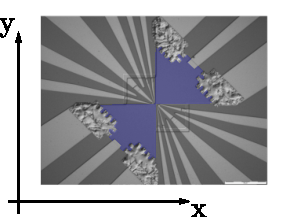
\includegraphics[width = 4 cm]{./intro/heterostructure_top_view}
			& &
			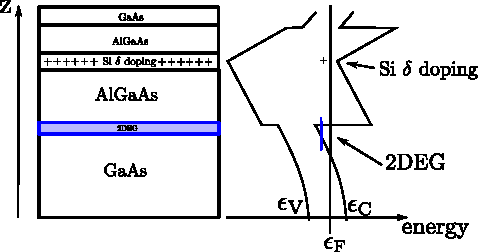
\includegraphics[width = 4 cm]{./intro/heterostructure_band_diagram} \\
			(c) & &  & \\
			& 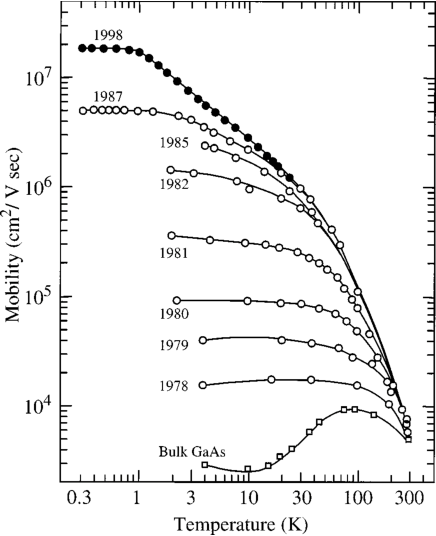
\includegraphics[width = 4 cm]{./intro/high_mobility}
			& &
			
		\end{tabular}
	\end{center}
	
	\caption{\textbf{High mobility 2D electron gas.} (a) The picture is a top view of the sample used in this manuscript where the surface colorized in blue is the 2D electron gas. (b) The schematic represents the different layers used to confine the electron gas in a two dimensional interface where the energy of the conduction band $\epsilon_{C}$ forms a quantum well as shown on the plot of energy as a function of the layer. (c) Graph from \cite{stormer1999nobel} that shown the increase of mobility in 2D electron gas with the development of the modulation doping technique based on the separation of donors and 2D electron gas in different layers of the semi-conductor heterostructure.}
	\label{fig: 2DEG}
\end{figure}

All the experiments are performed in a 2D electron gas of high mobility, the confinement of charge carriers in low dimensions allows the interaction effect.
The phenomena of integer and fractional quantum Hall effect in which the electronic transport is studied occur in two dimension, so the electrons involved in the transport are just moving in a plan.
This plan is colorized in blue in the sample picture shown in panel (a) of figure Fig.\ref{fig: 2DEG}.
These electrons are confined at an interface between two layers of semiconductors of AlGaAs and GaAs in a heterostructure, a diagram of the principal layer of the heterostructure is drawn in panel (b) of figure Fig.\ref{fig: 2DEG}.
This diagram shows in blue the plane of electrons called 2D electron gas, the modulation doping technique separates the donors which are Si atoms in a different layer than the electrons which are trapped in a quantum well between the GaAs layer of low energy conduction band and the attraction Si donors but in a AlGaAs layer of high energy conduction band.
This separation technique enables to made samples that achieve a high mobility of electrons at low temperature, the graph in panel (c) of figure Fig.\ref{fig: 2DEG}, presents the improvement other the years of the mobility of the 2D electron gas thanks to this technique, a high mobility is an other characteristic needed to observe interaction effects.


\begin{figure}[hptb]
	\begin{center}
		\begin{tabular}{c c c c}
			(a) & & (b) & \\
			& 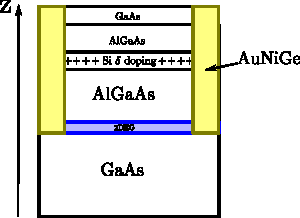
\includegraphics[width = 4 cm]{./intro/ohmic_contact_cut_view}
			& &
			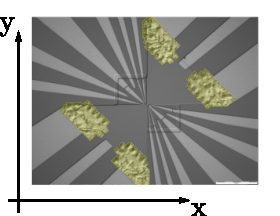
\includegraphics[width = 4 cm]{./intro/ohmic_contact_top_view} \\
		\end{tabular}
	\end{center}
	
	\caption{\textbf{Ohmic contacts that performed electrical connection with the 2D electron gas.} (a) The yellow rectangles are a schematic of the conductive alloy of AuNiGe diffused through all the layers of the heterostructure to reach the 2D electron gas. (b) The ohmics contacts on the sample top view are enhanced by a yellow false color. The size and the shape of the ohmic contacts increase the length between the electron gas and the alloy to have a better connection.}
	\label{fig: ohmic contact}
\end{figure}
 
Electrical connections with this 2D electron gas are made with different techniques, an ohmic contact is made of an alloy of AuNiGe that is diffused through the heterostructure and connects wires with the electron gas, a gate is a metallic deposit on top of the heterostructure which is capacitively coupled to the electron gas.
The electrical connections are used to manipulate the edges of the sample, indeed in the quantum Hall regime ballistic conductors appear at the edge of the sample called edge channels.
The ohmic contacts allow to directly connect the wire with the edge channels and to drive continuous current as well as high frequency current in the conductor.
This connection is made by an alloy of AuNiGe represented in the panel (a) of figure Fig.\ref{fig: ohmic contact} which is the conductive part that connect the top part of the sample with the electron gas in the heterostructure.
The top view in panel (b) of figure Fig.\ref{fig: ohmic contact} shows that the ohmic contacts are big compared to the electron gas size in order that the length of the edge of the electron gas along the ohmic contact is long enough to have a good connection with the edge channels. 
%They are also the connection used to connect a point of the edge channels to the ground.

\begin{figure}[hptb]
	\begin{center}
		\begin{tabular}{c c c c}
			(a) & & (b) & \\
			& 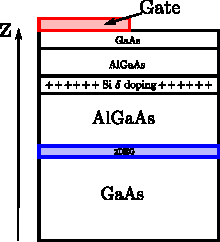
\includegraphics[width = 4 cm]{./intro/gate_cut_view}
			& &
			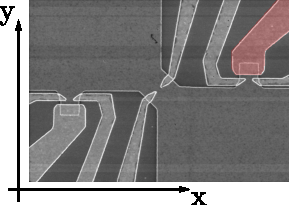
\includegraphics[width = 4 cm]{./intro/gate_top_view} \\
		\end{tabular}
	\end{center}
	
	\caption{\textbf{Gate coupled capacitively to the edge channel.} (a) The schematic shows that the gate in red is separated from the electron gas by the heterostructure, so the coupling is capacitive. (b) The gate enhanced in red is used in this manuscript to drive high frequency signal at the edge channel below.}
	\label{fig: gate}
\end{figure}

The gates can drive current in the conductor only for high frequency because they are capacitively to the edge of the electron gas and so to the edge channels.
The panel (a) of figure Fig.\ref{fig: gate} schematize the insulating layers of the heterostructure between the gate and the edge channel, and the panel (b) is a zoom on the center of the sample where the gate is enhanced in red.
In the manuscript this gate is used to add signals in the GHz frequency range to the edge channel.

\begin{figure}[hptb]
	\begin{center}
		\begin{tabular}{c c c c}
			(a) & & (b) & \\
			& 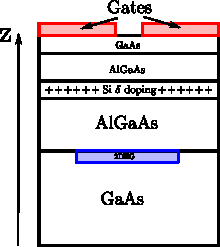
\includegraphics[width = 4 cm]{./intro/quantum_point_contact_cut_view}
			& &
			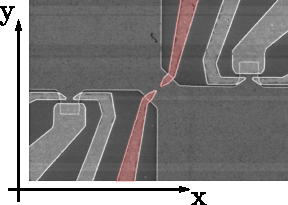
\includegraphics[width = 4 cm]{./intro/quantum_point_contact_top_view} \\
			(c) & &  & \\
			& 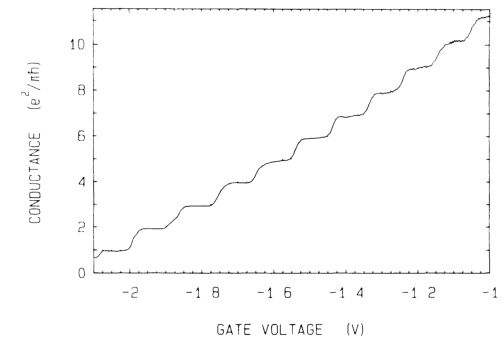
\includegraphics[width = 4 cm]{./intro/quantum_of_conductance}
			& &
			
		\end{tabular}
	\end{center}
	
	\caption{\textbf{Central quantum point used as an electronic beam-splitter.} (a) The schematic represents the electron gas in blue whose width decrease because the gates repeal the electron gas. (b) On the picture of the sample the two gates of the quantum point contact are colorized in red and are located at the narrower part of the electron gas to be able to connect or separate fully the two sides of the electron gas. (c) Graph from \cite{van1988quantized} of the conductance through a quantum point contact as a function of gate voltage. The gate voltage adjust the width of the quantum point contact which is smaller as the voltage is more negative. The conductance presents steps of twice the quantum of conductance each times two spin degenerate mode of electron can pass through the width of the quantum point contact.}
	\label{fig: qpc}
\end{figure}

They are also used with continuous voltage in the center of the sample, with a sufficiently negative voltage the gates repeal the electron gas below them, this allows controlling the geometry of the electron gas.
This control is used in the quantum point contact, this part is at the center of the sample where the electron gas is narrow and above it two gates can control its width up to the complete separation of the electron gas in two distinct parts, as one can notice on panels (a) and (b) of figure Fig.\ref{fig: qpc}.
The control of the width of the quantum point contact is used to control the transmission of electrical charges through it.
When the width of the quantum point contact is of the order of the Fermi wavelength of charges few electronic modes exist in the center of the electron gas, and by controlling the width, the gates control the number of modes and so the number of edge channels transmitted or reflected.
The conductance of the quantum point contact as a function of the voltage applied to the gates, as shown in figure Fig.\ref{fig: qpc} panel (c), is a measurement of the number of transmitted edge channels through the quantum point contact, and the curve exhibits steps of a quantum of conductance at each edge channel transmitted.
The voltage of the gates can also be set at a value between two steps of conductance, and at this voltage the last edge channel is then partially transmitted and reflected.
The quantum point contact is analogue to an electronic beam splitter for two edge channels coming from opposite sides of the quantum point contact and outgoing to two opposite edge channels with an adjustable transmission and reflection rate.

\begin{figure}[hptb]
	\begin{center}
		\begin{tabular}{c c c c}
			(a) & & (b) & \\
			& 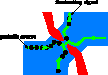
\includegraphics[height = 4 cm]{./intro/hom_shot_noise}
			& &
			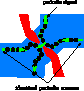
\includegraphics[height = 4 cm]{./intro/hom_noise_reduction} \\
			(c) & &  & \\
			& 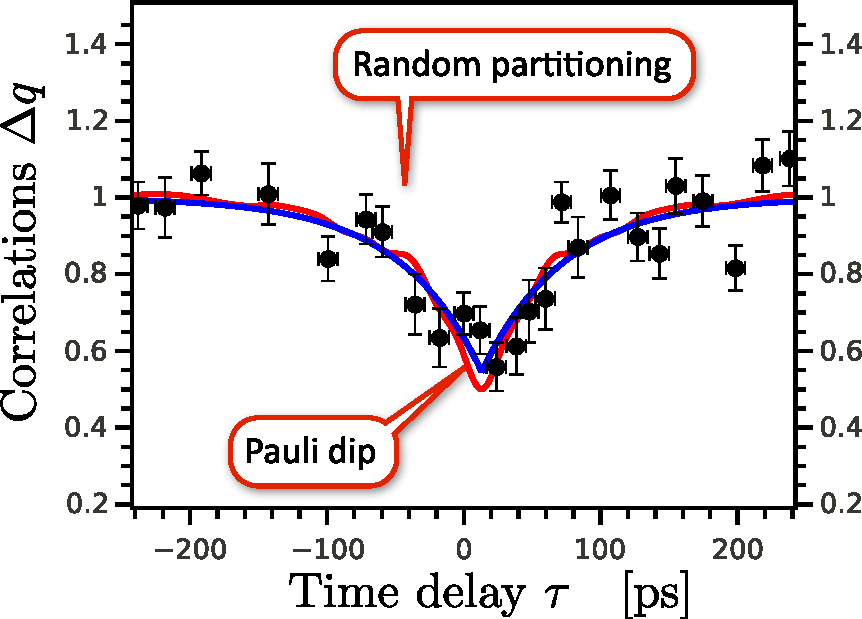
\includegraphics[width = 4 cm]{./intro/hom_measure}
			& &
			
		\end{tabular}
	\end{center}
	
	\caption{\textbf{Schematic of Hong-Ou-Mandel interferometer.} (a) In this schematic a train of periodic charges represented by black dots are emitted in a edge channel. They are randomly reflected or transmitted by the quantum point contact, so a randomly fluctuated signal called shot noise is generated in the output edge channels. (b) In this schematic two identical sources emit the same train of periodic charges. The signals in the output edge channels are not random but periodic since at each period  exactly one charge is reflected or transmitted in the output edge channels. The shot noise is suppressed, it is the Hong-Ou-Mandel interference effect. (c) Graph from \cite{bocquillon2013} where the correlation $\Delta q$ are the measured noise in one output edge channel normalised as a function of the time delay between the two sources emission. The time delay allows to control if the sources are identical or not, and the noise decrease when both sources are identical as expected with the Hong-Ou-Mandel effect.}
	\label{fig: hom}
\end{figure}

The elements of the sample used in this manuscript are one quantum point contact at the center of the electron gas, four ohmic contacts connected to the two input edge channel of the quantum point contact and to its two output edge channel, and one gate above an input edge channel.
These elements are present in the sample geometry of an electronic Hong-Ou-Mandel interferometer where two electrons sources emit a single electron at the inputs of the central quantum point contact. 
The central quantum point contact acts as a beam splitter and an incoming electron can be randomly transmitted or reflected to an output edge channel, so when electrons are periodically emitted in an incoming edge channel, they are partitioned in the two outputs channels where we get a randomly fluctuating signal called shot noise as drawn on panel (a) of figure Fig.\ref{fig: hom}.
This shot noise is suppressed when two indistinguishable electrons are emitted in the two inputs edge channel of the quantum point contact, the fermionic statistic prevent the identical electrons to exit in the same channel, this implies that there is always one electron at each output edge channel as drawn on panel (b) of figure Fig.\ref{fig: hom}.
The measurement of the shot noise in an output channel gives information about the overlap of the two electronic states in the input edge channels, the experience demonstrating this electronic Hong-Ou-Mandel effect has been realized in \cite{bocquillon2013} and the main measurement is plotted on panel (c) of figure Fig.\ref{fig: hom} and used to study decoherence and fractionalization of single electron emission \cite{marguerite2016decoherence}.
The measurement of noise will be used in the three chapters of this manuscript to deduce information on the electronic states.

%%%%%%%%%%%%%%%%%%%%%%%%%%%%%%%%%%% TEXT BODY %%%%%%%%%%%%%%%%%%%%%%%%%%%%%%%%%
\mainmatter

%% !TeX encoding = UTF-8
% !TeX spellcheck = en_GB
% !TeX root = mythesis.tex
\chapter{Fractionally charged quasi-particle signature in microwave photons emission}

%Le projet de charge fractionnaires détectée par bruit RF


%\begin{enumerate}
%	\item Le set-up de mesure de bruit
%	\item Les calculs d'Ines-Safi
%	\item Les résultats de conductances et de bruit BF
%	\item Les résultats de bruit RF
%\end{enumerate}

\section{\texorpdfstring{...}{...}}

\subsection{\texorpdfstring{...}{...}}

% l'effet Hall classique donne des info sur porteurs de charge

\begin{figure}[hptb]
	\begin{center}
		\begin{tabular}{c c c c}
			(a) & & (b) & \\
			& 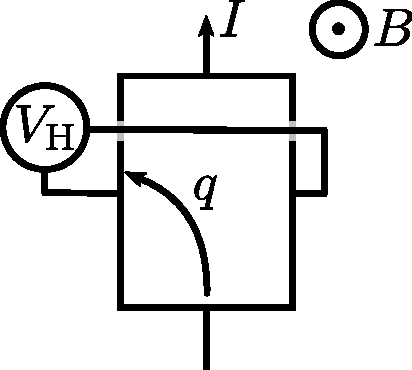
\includegraphics[width = 4 cm]{./chap2/effet_Hall_classique}
			& &
			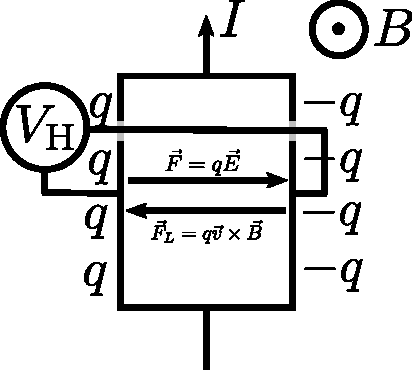
\includegraphics[width = 4 cm]{./chap2/effet_Hall_classique_bis} \\
		\end{tabular}
	\end{center}
	
	\caption{\textbf{title.}}
	\label{fig: effet Hall classique}
\end{figure}

The Hall effect is usually used to get charge $q$ and density $n$ of the charge carriers in a semiconductor.
The application of a perpendicular magnetic field $\vec{B}$ to a 2D conductor leads to the appearance of a voltage difference $V_{\mathrm{H}}$ perpendicularly to the current flow $I$.
The charges $q$ flowing through the semiconductor are deviated by the magnetic field with the Lorentz force $\vec{F}_L = q\vec{v}\times\vec{B}$.
As they are deviated perpendicularly to the current flow direction given by $q\vec{v}$, there is an accumulation of charges on the edges of the sample.
These charges on the edge of the sample create a voltage difference perpendicularly to the current, the Hall voltage $V_{\mathrm{H}}$.
The electrostatic force created by the Hall voltage balances the Lorentz force in the permanent regime, and one get the relation between the Hall voltage and the current \eqref{eq: Hall law} which introduces the Hall resistance \eqref{eq: Hall resistance}.

\begin{equation}
V_{\mathrm{H}} = R_{\mathrm{H}}I \label{eq: Hall law}
\end{equation}

\begin{equation}
R_{\mathrm{H}} = \frac{B}{nq} \label{eq: Hall resistance}
\end{equation}

with $n$ the surface density of charge, $q$ the charge of carriers, $B$ the magnetic field.
The Hall resistance is proportional to the magnetic field applied and the measurement of the proportionality coefficient gives the information of $q$ and $n$ on the charge carriers.
The 2D conductor used in this manuscript is an interface between two semiconductors of AlGaAs and GaAs, and the charge carrier are electrons of charge $q = -e$ given by Si donors whose number determines the surface density $n = 2.10^{11}$ cm$^{2}$.

\subsection{\texorpdfstring{...}{...}}

% si on va plus haut en champ on a effet Hall quantique entier, là on prend des infos avec le bruit BF et RF, on a fait ça pour régime entier


\begin{figure}[hptb]
	\begin{center}
		\begin{tabular}{c c c c}
			(a) & & (b) & \\
			& 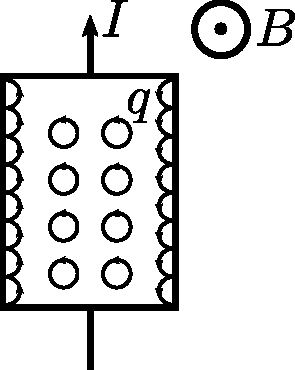
\includegraphics[width = 4 cm]{./chap2/effet_Hall_semi_classique} &
			& 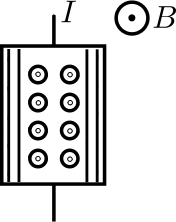
\includegraphics[width = 4 cm]{./chap2/effet_Hall_quantique}
		\end{tabular}
	\end{center}
	
	\caption{\textbf{title.} \textbf{(a)}  \textbf{(b)}}
	\label{fig: effet Hall quantique}
\end{figure}

\begin{figure}[hptb]
	\begin{center}
		\begin{tabular}{c c c c}
			(a) & & (b) & \\
			& 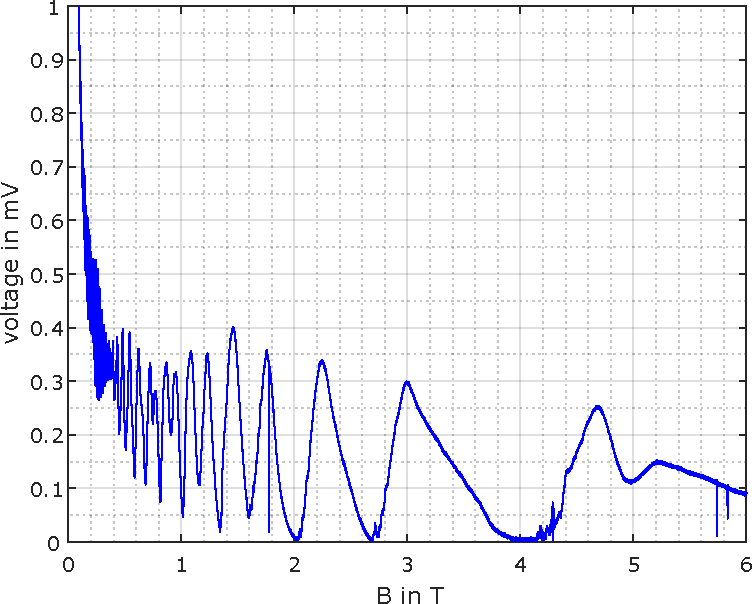
\includegraphics[width = 6.5 cm]{./chap2/backscattered_current} &
			& 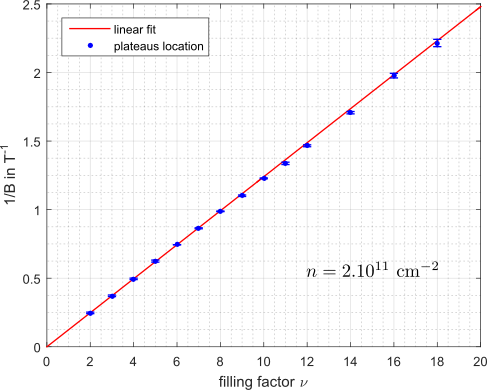
\includegraphics[width = 6.5 cm]{./chap2/B_vs_nu}
		\end{tabular}
	\end{center}
	
	\caption{\textbf{title.} \textbf{(a)}  \textbf{(b)}}
	\label{fig: backscattered current}
\end{figure}

For a high mobility 2D sample and at cold temperature one can observe that the Hall resistance is quantified for specific values which are fractions of the quantum of resistance \eqref{eq: quantum Hall resistance}, and the Hall resistance as a function of the magnetic field gives plateaus around corresponding magnetic field.

\begin{equation}
R_{\mathrm{H}} = \frac{1}{\nu}\times\frac{h}{e^{2}} \label{eq: quantum Hall resistance}
\end{equation}

with $\nu$ an integer number.
This quantification of the Hall resistance is the signature of the integer quantum Hall effect \cite{von1986quantized}.
In this regime, the electron system cannot be described by classical trajectories governed by Lorentz force, but is described by Landau levels.
The Landau levels are distributed in bands of discrete energies separated by the cyclotron pulsation $\hbar\omega_{c}$ and the Zeeman splitting $\hbar\omega_{z}$.
The cyclotron pulsation and the Zeeman splitting are proportional to the magnetic field $B$ which controls the number of bands below the Fermi energy.
This number of filled bands below the Fermi energy is the filling factor $\nu$ which is the integer number dividing the quantum of resistance in equation \eqref{eq: quantum Hall resistance}.
In this new regime, the electron transport is carried by $\nu$ states at the edge of the channel.
These states, called edge channel, are ballistic and chiral, so the longitudinal resistance of the sample is suppressed when the current is only carried by these edge channels, since the carriers are never backscattered.
In figure Fig. \ref{fig: backscattered current} panel (a), the backscattered voltage is measured as a function of the magnetic field $B$, and it reaches zero values.
The relation between the magnetic field and the filling factor \eqref{eq: B vs nu} is found by equations \eqref{eq: Hall resistance} and \eqref{eq: quantum Hall resistance}.

\begin{equation}
\frac{1}{B} = \frac{e}{nh}\nu \label{eq: B vs nu}
\end{equation}

By numbering the zeros of the panel (a), the panel (b) of figure Fig. \ref{fig: backscattered current} shows the inverse of the magnetic field as a function of the filling factor.
The data points are distributed on a linear curve as given by \eqref{eq: B vs nu}, and the slope of the fit gives the density of $n = 2.10^{11}$ cm$^{-2}$.
On the graph the filling factors 13, 15, and 17 are missing because for low magnetic field the Zeeman splitting is not big enough to separate Landau levels of different spin.

\subsubsection*{...}

%le bruit basse fréquence

In the quantum Hall effect, the electronic transport takes place on the edge channels.
To characterize the charge carriers in the edge channels, the low frequency noise can be used.
Schottky has demonstrated in \cite{schottky1918regarding} that the random partitioning of an electrical current generates a low frequency shot noise proportional to the charge of the carriers.


\subsubsection*{...}

\begin{figure}[hptb]
	\begin{center}
		\begin{tabular}{c c c c}
			(a) & & (b) & \\
			& 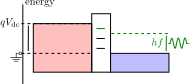
\includegraphics[width = 6.5 cm]{./chap2/noise_schematics_a} &
			& 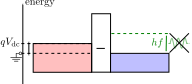
\includegraphics[width = 6.5 cm]{./chap2/noise_schematics_b}  
		\end{tabular}
	\end{center}
	
	\caption{\textbf{title.} \textbf{(a)}  \textbf{(b)} }
	\label{fig: principle schematics}
\end{figure}

Another method to determine the charge of carriers in the edge channel is to measure the high frequency noise.
The principle of this measurement is based on the Pauli exclusion principle and the quantification of the energy of microwave photons.
A DC voltage difference $V_{dc}$ is applied on the leads of a tunnel barrier, it shifts the Fermi level between the two leads of $qV_{\mathrm{dc}}$ with $q$ the charge of carriers.
This is drawn on figure Fig. \ref{fig: principle schematics} where the two leads are plotted in red and blue.
Charge carriers can tunnel through the tunnel barrier only between zero energy and $qV_{\mathrm{dc}}$, for energies higher than $qV_{\mathrm{dc}}$ there are no particles, for energies below the reference level all states are occupied on both leads so the Pauli exclusion principle avoid the tunnelling of charges.
As particles tunnels in an energy window of $qV_{\mathrm{dc}}$, the available energy in the system is bounded by $qV_{\mathrm{dc}}$.
The noise at frequency $f$ is the fluctuation of the signal at frequency $f$ in the microwave cable connected to the sample.
This signal can fluctuate only if microwave photons at frequency $f$ are emitted or absorbed by the cable, and the quantification of the energy of microwave photons set the energy exchange to be at least of $hf$ the energy of one photon.
In figure Fig. \ref{fig: principle schematics} the two panels shows two situations, in the panel (a) available energy $qV_{\mathrm{dc}}$ is higher than one microwave photon energy $hf$ so high frequency noise is generated, in the panel (b) $qV_{\mathrm{dc}}$ is below $hf$ so the high frequency noise is suppressed.
This transition between the regime without high frequency noise and with high frequency noise is obtained for a DC voltage $V_{dc} = \frac{hf}{q}$.
By measuring this transition, one gets a direct measurement of the charge $q$ since $V_{\mathrm{dc}}$ and $f$ are set by measurement instruments and not the properties of the sample such as the conduction of the tunnel barrier. 
This technique has been experimentally used in different conductors \cite{schoelkopf1997frequency,zakka2007experimental,gabelli2009high} revealing the elementary charge $q = e$ of electrons carrying the current in these systems.


\subsection{\texorpdfstring{...}{...}}

% et dans l'effet Hall quantique fractionnaire les porteurs ont la propriétée surprenante d'avoir une charge fractionnaire, ça été sondé avec le bruit BF, nous on fait ça avec du bruit RF en émission, c'est complémentaire aux mesures d'absorption de Kapfer.

\begin{figure}[hptb]
	\begin{center}
		\begin{tabular}{c}
			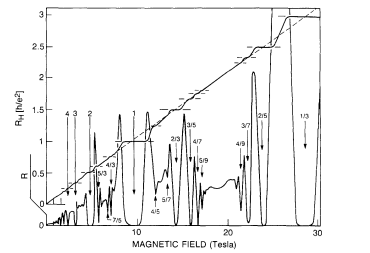
\includegraphics[width = 6.5 cm]{./chap2/fractional_Hall_resistance}
		\end{tabular}
	\end{center}
	
	\caption{\textbf{title.} }
	\label{fig: effet Hall quantique fractionnaire}
\end{figure}

The magnetic field can be increased such that the filling factor $\nu$ reaches values below one.
In this regime, the backscattered voltage drops also when the filling factor equals specific fractions such as $\dfrac{2}{3}$ or $\frac{1}{3}$, this characterizes the fractional quantum Hall effect.
The Hall resistance and the magnetic field at which this regime is reached is still determined by the fractional filling factor in equations \eqref{eq: quantum Hall resistance} and \eqref{eq: B vs nu}.
The strong electronic interactions change other properties of the electronic system such as the charge of carriers, indeed one can consider that the current is carried by quasiparticles of fractional charges.
These fractional charges have been measured through low frequency noise
by different experimental techniques.
The first techniques \cite{saminadayar1997observation,de1998direct,reznikov1999observation,bid2009shot,hashisaka2015shot} measure the low frequency noise generated by a quantum point contact when there is a DC voltage difference is applied at its inputs.
The output noise depends on both the conductance of the quantum point contact and on the charge of the carriers.
Another experimental technique realized in \cite{kapfer2019josephson,kapfer2018dynamic} still measures the output low frequency noise, but in addition to DC voltage difference applied to the inputs an extra RF sinus voltage is sent.
The added RF sinus voltage generates a photo-assisted shot noise from which the charge of carriers can be deduced as a function of the sinus frequency.
In the integer quantum Hall regime, the RF sinus of frequency $f$ modifies the electronic occupation by energy steps of size $hf$, these steps implies a slope variation of the noise when $qV_{\mathrm{dc}}$ reaches the same values, with $V_{\mathrm{dc}}$ the DC voltage applied.
The results of the article \cite{kapfer2019josephson} demonstrate that the same effect is obtained in the fractional regime with only $q$ equals a fractional charge.
This experiment investigates how a RF excitation is absorbed by the electronic system in the fractional regime.
This chapter presents a complementary experiment by measuring the emitted RF noise in the fractional regime.
As explained in the previous subsection and shown in \cite{schoelkopf1997frequency,zakka2007experimental,gabelli2009high}, one can deduce the charge of carriers by measuring the emitted high frequency noise.
This measurement of high frequency excitations also allows measuring the charge of carriers as a function of frequency and a DC voltage, without depending on the precise value of quantum point contact conductance.
When the excitations are electrons, the explanation of the results uses the Pauli exclusion principle, but in the fractional regime the excitations are anyons with a different statistic \cite{arovas1984fractional,halperin1984statistics,bartolomei2020fractional,nakamura2020direct}, so this chapter shows similar results without this principle \cite{haldane1991fractional}.


\section{\texorpdfstring{Experimental set-up}{Experimental set-up} \label{sec: Experimental set-up chap2}}

In this section the experimental techniques are detailed.
With a first part that describes the sample used and the low frequency characterizations and a second part that describes the high frequency noise measurement technique, whose experimental set-up is drawn in figure Fig. \ref{fig: le set-up chap2}.

\subsection{Low frequency set-up}

\begin{figure}
	\centering
	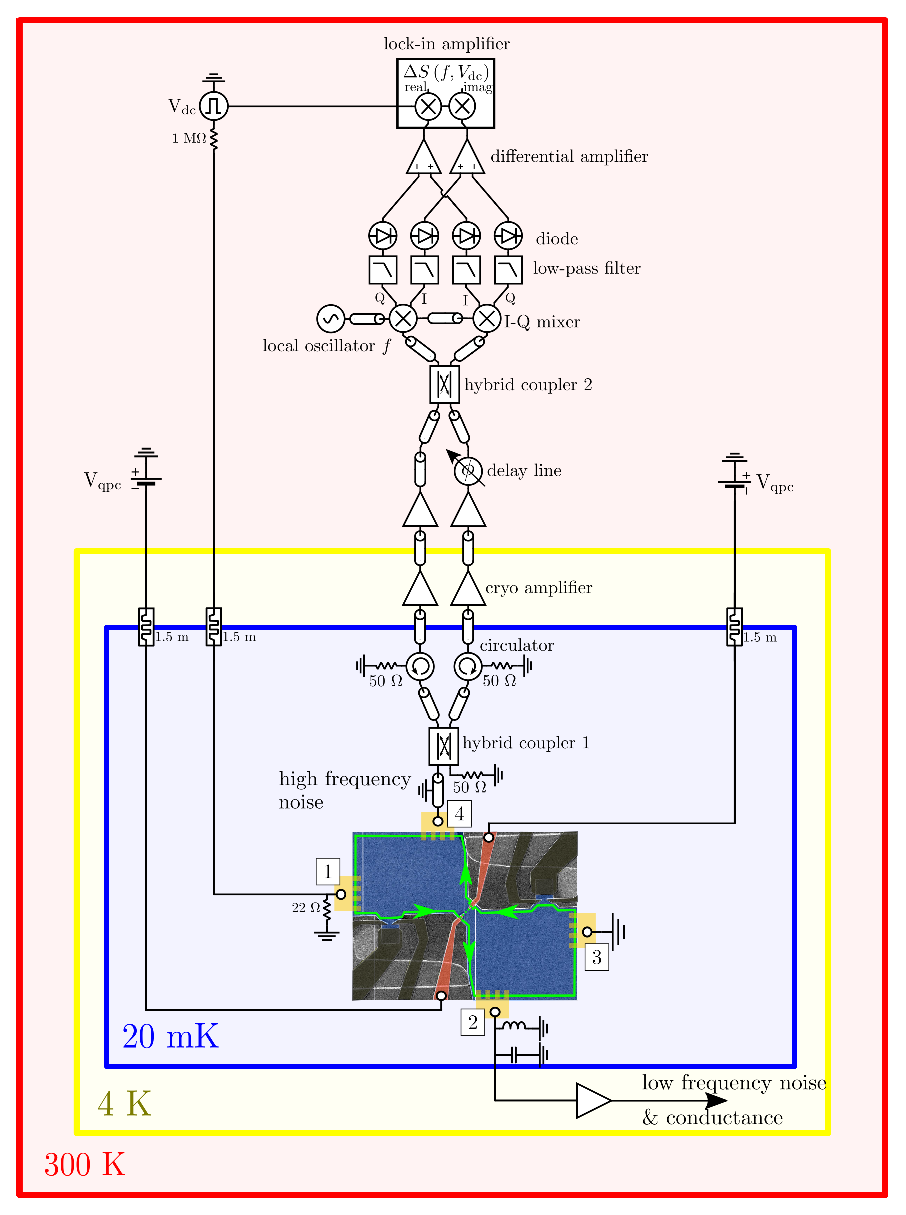
\includegraphics[width = 12cm]{./chap2/set-up_bruit_RF_pour_charge.eps}
	\caption{\textbf{Experimental set-up of high frequency noise measurement.} This schematic is separated in four regions: the red part at 300 K which is the exterior of the dilution fridge; the yellow part at 4K and the blue part at 20 mK which are inner stage of the dilution fridge; the sample SEM picture in false color which is the object studied. On the sample the 2D electron gas is coloured in blue, the quantum point contact gates in red, the Ohmic contacts are added in yellow, the outer edge-channel in green. DC voltage sources for gate voltages $V_{\mathrm{qpc}}$ are represented by a battery. The voltage source of DC bias $V_{\mathrm{dc}}$ is a very low frequency $\sim 230$ Hz squared voltage between 0 and $V_{\mathrm{dc}}$. The high frequency measurement set-up is detailed with the microwave Mach-Zehnder interferometer including amplifiers between the two hybrid couplers, the local oscillator with I-Q mixers and diodes to detect the noise power at a specific frequency, and the lock-in amplifier which demodulates the noise power generated by the bias voltage at the very low frequency of 230 Hz.  \label{fig: le set-up chap2}}
\end{figure}

The first measurements to characterize conductance and charge carriers are low frequency measurements.
The measurement lines used to perform them are minimally sketched on the figure Fig. \ref{fig: le set-up chap2} of this chapter, but it is fully drawn in the next chapter in figure Fig. \ref{fig: le set-up} and detailed in appendix in figure Fig. \ref{fig: output LF line}.
This organization is due to the fact that new measurements performed in this chapter are in the radio-frequency band, whereas the low frequency lines are used to perform new measurements in the next chapter.

\subsubsection*{DC voltage applied.}

\begin{figure}[hptb]
	\begin{center}
		\begin{tabular}{c c c c}
			(a) & & (b) & \\
			& 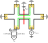
\includegraphics[width = 6.5 cm]{./chap2/Hall_bar_split_gate_open} &
			& 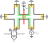
\includegraphics[width = 6.5 cm]{./chap2/Hall_bar_split_gate_close} \\
			(c) & & & \\
			& 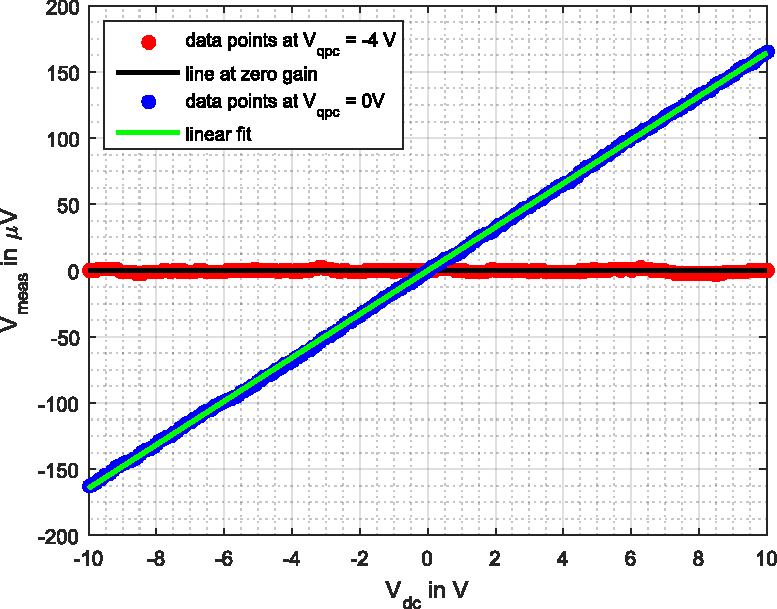
\includegraphics[width = 6.5 cm]{./chap2/DC_line_gain} &
			& 
			
		\end{tabular}
	\end{center}
	
	\caption{\textbf{Calibration at low temperature of DC voltage input line.} \textbf{(a)} Schematic of the Hall bar used to calibrate the attenuation of the bias voltage $V_{\mathrm{dc}}$ line. The limits of the 2D electron gas is delimited in black line, the Ohmic contacts are in yellow, the edge-channel in green, and the top gate in red. In this panel the voltage applied to the top gate is $V_{\mathrm{qpc}} = 0$ V, so the edge-channel is fully transmitted. \textbf{(b)} Same schematic as in previous panel but with a negative voltage applied to the gate $V_{\mathrm{qpc}} = -4$ V, this implies that the edge-channel is fully reflected by the top gate. \textbf{(c)} Voltage $V_{\mathrm{meas}}$ measured like on above panels as a function of bias voltage $V_{\mathrm{dc}}$. Data points in red are measured in panel (b) configuration, the measured voltages are independent of applied voltage $V_{\mathrm{dc}}$ and equal to zero as shown by the black line. Data points in blue are measured in the panel (a) case where, as the edge-channel is a ballistic conductor, the measured voltage equals the applied voltage in the edge-channel. The slope of the linear fit in green line is the measurement of the attenuation of the input line for $V_{\mathrm{dc}}$. This slope equals $1.64 \times 10^{-5}$.}
	\label{fig: DC line gain}
\end{figure}


The only sources used in this chapter are a DC voltage sources $V_{\mathrm{dc}}$ and $V_{\mathrm{qpc}}$, which are attenuated and thermalised.
The thermalisation of the lines occurs at the coldest stage thanks to a 1.5 m meander embedded in a copper powder filter.

One of the sources, carrying the voltage $V_{\mathrm{dc}}$, is connected to the Ohmic contact 1. 
It is attenuated by a voltage divider formed of a serial 1 M$\Omega$ resistor at room temperature and a parallel 22 $\Omega$ resistor at cold temperature contributing to the thermalisation of $V_{\mathrm{dc}}$.
As the DC voltage source used is limited by a 10 V range, this attenuation enables to work in a voltage range around 200 $\upmu$V at the sample level.
The 1 M$\Omega$ serial resistor is changed for a 0.68 M$\Omega$ resistor to reach at the sample a 300 $\upmu$V range and a 0.47 M$\Omega$ resistor to get a 500 $\upmu$V range.
To know precisely the voltage $V_{\mathrm{dc}}$ applied at the sample level, the voltage divider is calibrated at low temperature by replacing the sample by a Hall bar with a gate between the contacts, as in figure Fig. \ref{fig: DC line gain}.
For the calibration only, the voltage source is differential and two series resistors of total resistance $2\times 0.68$ M$\Omega$ contributes to the voltage divider.
When there is no voltage applied to the gate $V_{\mathrm{qpc}} = 0$ V, the edge channels are perfectly transmitted through the gate.
This implies that the DC voltage measured at the following Ohmic contact on the edge channel is the voltage at the sample level, as on the panel (a).
A linear fit of the measured voltage as a function of the applied voltage gives the voltage divider at low temperature, as given by the green line on the panel (c).
When the gate voltage  $V_{\mathrm{g}}$ is enough negative, one can check that the measured voltage is constant at zero, as shown by red points on the panel (c).
The DC voltage source shifts the chemical potential of one edge-channel through an Ohmic contact compared to the grounded opposite one as shown by the two horizontal green arrow in figure Fig. \ref{fig: le set-up chap2}.

The two opposite edge-channels meet at the central narrowing of the 2D electron gas in blue in the figure.
By applying a negative voltage $V_{\mathrm{qpc}}$ on the two red gates, one can adjust the electron transmission through a tunnel barrier, called quantum point contact, between the two edge-channels at the narrowing.
As the voltage range applied to the gates is about -1 V, there is no attenuation at cold temperature of the voltage applied $V_{\mathrm{qpc}}$, but they are still thermalised by meanders.

\subsubsection*{Conductance measurement.}

To measure the transmission of the central quantum point contact, a lock-in amplifier adds a small sine voltage to the DC source with a bias-tee, and measures the transmitted signal through the quantum point contact amplified by the noise measurement line.
The measured signal is proportional to the quantum point contact conductance at the bias voltage $V_{\mathrm{dc}}$ by identifying the plateaus of conductance as a function of $V_{\mathrm{qpc}}$, one can deduce the coefficient of proportionality.
On the schematics, only one edge-channel is represented, but depending on the magnetic field applied perpendicularly to the sample the number and the nature of the edge-channels change.
This can be probed by the quantum point contact conductance measurement and by the low frequency noise measurement.

\subsubsection*{Low frequency noise measurement.}

\begin{figure}[hptb]
	\begin{center}
		\begin{tabular}{c c c c}
			(a) & & (b) & \\
			& 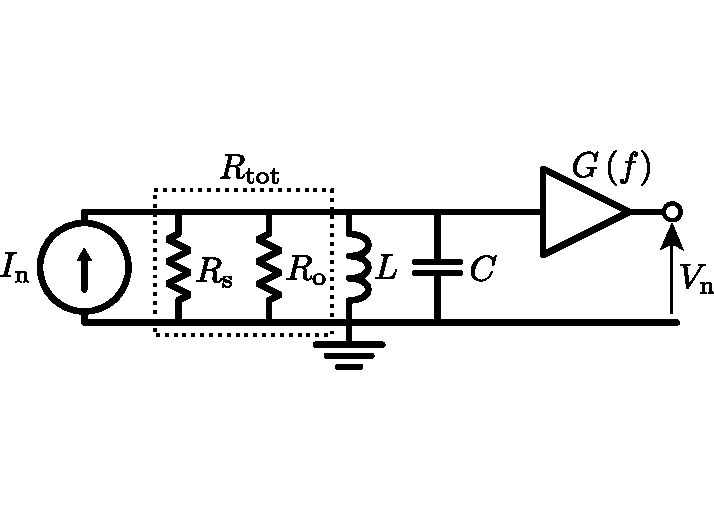
\includegraphics[width = 6.5 cm]{./chap2/gain_low_freq_noise} &
			& 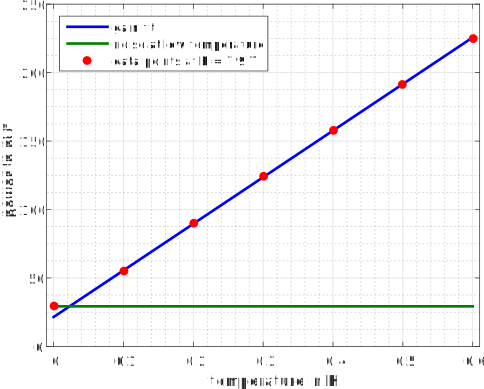
\includegraphics[width = 6.5 cm]{./chap2/temperature_calibration} \\
			(c) & & (d) & \\
			& 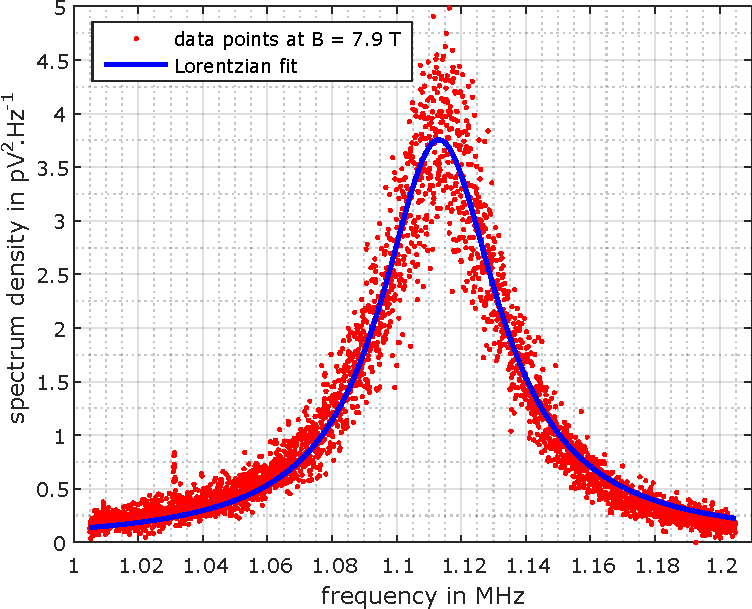
\includegraphics[width = 6.5 cm]{./chap2/noise_spectrum_nu_1} &
			& 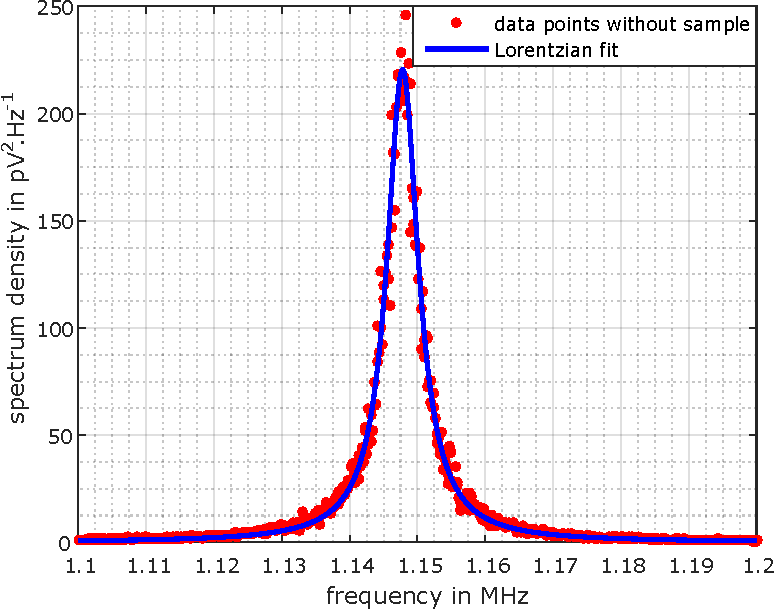
\includegraphics[width = 6.5 cm]{./chap2/noise_spectrum_open}
			
		\end{tabular}
	\end{center}
	
	\caption{\textbf{Low frequency noise measurement.} \textbf{(a)} The model of the measurement line is described by the drawn electronic circuit. The generated current noise $I_{\mathrm{n}}$ is distributed between the sample resistance $R_{\mathrm{s}}$, an added coil $L$, cables and amplifiers input capacitance $C$, a resistance $R_{\mathrm{o}}$ which models imperfection of the resonator. The voltage at their leads is amplified by amplifiers of gain $G$. \textbf{(b)} The power of the voltage noise $V_{\mathrm{n}}$ is plotted as a function of sample temperature. The resistance of the sample is fixed at $R_{\mathrm{s}} = \frac{h}{e^2}$ by the choice of the magnetic field $B = 7.9$ T. The data points at temperature above 100 mK are fitted by the blue line, its linear evolution is due to the increase of the thermal current noise. The lowest power measured at the lowest temperature is plotted by a red point at zero temperature and a green line. The crossing between the green and blue line gives the lowest temperature of electrons. \textbf{(c)} The measured power spectrum density is plotted as a function of frequency. It is the thermal noise of the sample of resistance $R_{\mathrm{s}} = \frac{h}{e^2}$ at a temperature of 600 mK. If the amplifiers gain is constant in the measurement bandwidth, the red data points are modelled by a Lorentzian resonance plotted in blue line. \textbf{(d)} The power spectrum density is measured without any sample connected.}
	\label{fig: low freq noise gain}
\end{figure}

The low frequency noise is measured at the Ohmic contact 2 see figure \ref{fig: le set-up chap2}.
First the core-less coil, which is connected in parallel, shifts with cable and amplifier input capacitances the measured noise at 1.1 MHz.
Then amplifiers and a vector spectrum analyser detects the noise spectrum at low frequency.
The calibration of the gain $G_{IV}^{2}$ of this measurement line is needed to get information on the system.
This gain is determined by three measurements plotted in figure Fig. \ref{fig: low freq noise gain}.
This determination procedure is explained in the following paragraphs with the example of a magnetic field of $B = 7.9$ T giving a filling factor $\nu = 1$.

The electrical model of these measurements is drawn on the panel (a), where a noise current source $I_{\mathrm{n}}$ is loaded by the sample resistance $R_{\mathrm{s}}$, the core-less coil $L$, the cable and amplifiers input capacitance $C$, and a resistor $R_{\mathrm{o}}$ taking into account the losses of the resonator.
The signal is then amplified with a gain $G$, to get the output voltage noise $V_{\mathrm{n}}$.
The first measurement consists of measuring with the vector spectrum analyser the power $P$ integrated on frequency of the voltage noise as a function of the temperature $T$ of the resistances.
The thermal excitations give a voltage noise spectrum density $S_{VV}$ proportional to the system temperature $T$ \eqref{eq: thermal spectrum density}:

\begin{equation}
S_{VV}\left(f\right) = \left|G\left(f\right)\right|^{2}\frac{4R_{\mathrm{tot}}k_{\mathrm{B}}T}{1+Q_{\mathrm{s}}^{2}\left(\frac{f}{f_{\mathrm{s}}}-\frac{f_{\mathrm{s}}}{f}\right)^{2}} \label{eq: thermal spectrum density}
\end{equation}

with $Q_{\mathrm{s}}$ and $f_{\mathrm{s}}$, the quality factor and resonance frequency of the set-up, and $R_{\mathrm{tot}}$ the total resistance formed by $R_{\mathrm{s}}$ and $R_{\mathrm{o}}$.

%On panel (b) the measured quantity as a function of temperature is the voltage noise power, which is the integral \eqref{eq: link power spectrum density} of the spectrum density.
Panel (b) represents measurements of the noise power $P$, which is the integral \eqref{eq: link power spectrum density} of the noise spectrum density, as a function of the temperature $T$.

\begin{equation}
P = \int_{f_{\mathrm{s}}-\frac{\Delta f_{\mathrm{s}}}{2}}^{f_{\mathrm{s}}+\frac{\Delta f_{\mathrm{s}}}{2}} S_{VV}\left(f\right)\mathrm{d}f \label{eq: link power spectrum density}
\end{equation}

On the measurement of figure Fig. \ref{fig: low freq noise gain} panel (b), we remark that the data points, in red points, can be fitted by a linear function $P = AT+B$, where the slope $A$ will be inversely proportional to the searched gain, and $B$ is the additional noise coming from the amplifiers.
The linear fit, in blue line, does not include the coldest point because we remark that below 40 mK the system temperature differs from the electrons temperature $T_{\mathrm{elec}} = ...$ mK.

The searched gain is the link between the measured power $P$ and the current noise spectrum $S_{II}$, given by \eqref{eq: link power current noise}, when the noise source is the shot noise generated at the quantum point contact.

\begin{equation}
P = \int_{f_{\mathrm{s}}-\frac{\Delta f_{\mathrm{s}}}{2}}^{f_{\mathrm{s}}+\frac{\Delta f_{\mathrm{s}}}{2}}\left|G\left(f\right)\right|^{2}\frac{R_{\mathrm{tot}}^{2}}{1+Q_{\mathrm{s}}^{2}\left(\frac{f}{f_{\mathrm{s}}}-\frac{f_{\mathrm{s}}}{f}\right)^{2}}S_{II}\mathrm{d}f \label{eq: link power current noise}
\end{equation}

At frequencies around 1 MHz, which are small compared to thermal excitations $\frac{k_{\mathrm{B}}T}{h} \sim 1$ GHz, the shot noise spectrum density does not depend on frequency, and thanks to the three above equations, the searched gain $G_{IV}^{2}$ is simply linked to the measured slope $A$ on the panel (b) by \eqref{eq: gain power to current noise}.

\begin{equation}
S_{II} = G_{IV}^{2}P \Rightarrow G_{IV}^{2} = \frac{4k_{\mathrm{B}}}{AR_{\mathrm{tot}}} \label{eq: gain power to current noise}
\end{equation}

In addition to the slope $A$, the gain $G_{IV}^{2}$ includes the total resistance of the sample resistance $R_{\mathrm{s}}$ in parallel with the open measurement chain resistance $R_{\mathrm{o}}$.
The sample resistance is known thanks to the quantization at each filling factor $\nu$ by $R_{\mathrm{s}} = \frac{h}{e^{2}\nu}$, but $R_{\mathrm{o}}$ has to be measured.
To do so we record the voltage noise spectrum density due to thermal noise with the sample connected in panel (c) and without the sample connected in panel (d).
From a Lorentzian fit of the resonance peak in the two measurements, we extract their quality factors and resonance frequencies, $Q_{\mathrm{s}}$ and $f_{\mathrm{s}}$ with sample, $Q_{\mathrm{0}}$ and $f_{\mathrm{0}}$ open loaded.
The resonance frequency is higher when the sample is removed because there are less cable and the capacitance decreases, but as the inductance remains constant we deduce the total resistance by equation \eqref{eq: link Rtot Rs}.

\begin{equation}
R_{\mathrm{tot}} = R_{\mathrm{s}}\left(1-\frac{Q_{\mathrm{s}}f_{\mathrm{s}}}{Q_{\mathrm{o}}f_{\mathrm{o}}}\right) \label{eq: link Rtot Rs}
\end{equation}

With this method we calibrate the gain $G_{IV}^{2}$ for all values of $\nu$ and we get for example $G_{IV}^{2} = ...$ S$^{2}$.Hz$^{-1}$.

\subsection{High frequency measurements}

The high frequency noise set-up is detailed in figure Fig. \ref{fig: le set-up chap2}, it is based on the set-up developed in \cite{parmentier2011high,parmentier2010short,engelbrecht1965wide,bisognin2019microwave}.
In this set-up the components to measure the noise at a chosen frequency are the I-Q mixers, low-pass filters, and the diodes.
The I-Q mixers multiply the signal by a local oscillator at the chosen frequency $f$, they perform a frequency translation in Fourier domain by shifting the signal around frequency $f$ towards DC signals.
The low-pass filters select the frequency bandwidth in which the noise is integrated, by suppressing all signals above their frequency cut-off.
The diodes square the noise and their dc signal outputs are proportional to the noise power.
The rest of the set-up, the amplifiers, the microwave Mach-Zehnder between the two hybrid couplers, and the modulation with the lock-in amplifier, enables to reach enough sensitivity to extract the signal from noise.
Indeed the order of magnitude of the measured signal around 7 GHz of partitioning elementary charges $e$ is $S_{\mathrm{meas.}} \sim e^{2}f \sim 1.10^{-29}$ A$^{2}.$Hz$^{-1}$.
This noise is compared to the thermal noises of the 50$\Omega$ impedance of the amplifiers at 4 K, which is around $S_{\mathrm{th.}} \sim 4Gk_{\mathrm{B}}T \sim 4.10^{-24}$ A$^{2}.$Hz$^{-1}$, and to the noise of the 50$\Omega$ resistor at the coldest part at 20 mK, which is of the order of $S_{\mathrm{th.}} \sim 2.10^{-26}$ A$^{2}.$Hz$^{-1}$.
So even at the lowest temperature, the thermal noise is three orders of magnitude above the measured signal.
The amplifiers amplify the signal above the room temperature thermal noise.
The microwave Mach-Zehnder reduces the amplifier noise by splitting it equally on the four diodes, so it is subtracted continuously by the differential amplifiers, whereas the signal is distributed only on the input "$+$" of the differential amplifiers.
Finally, the excitation modulation with a low frequency square function generator and the demodulation by the lock-in amplifier, enable to have enough stability to average until the measurement reaches enough sensitivity.
If one reads the measurement line schematics step by step, first the edge-channel is connected to a 50 $\Omega$ cable through an Ohmic contact.
This cable is connected to one input of hybrid coupler 1 and the other input is loaded with a 50 $\Omega$ resistor.
Let $a$ and $b$ be the signal at the two inputs, and $c$ and $d$ the signal at the outputs \eqref{eq: hybrid coupler 1}.

\begin{align}
	c & =  \frac{a+ib}{\sqrt{2}} \\
	d & =  \frac{ia+b}{\sqrt{2}} \label{eq: hybrid coupler 1}
\end{align}

The two amplifying chains are of gain $g_{1}$ and $g_{2}$, and they add the noises $\epsilon$, $\zeta$, the delay line balance the phase between the two chains by a phase $\theta$, this gives the signals after amplification $e$, $f$ \eqref{eq: amplifiers}.

\begin{align}
	e & =  g_{1}e^{i\theta}c+\epsilon \\
	f & =  g_{2}d+\zeta \label{eq: amplifiers}
\end{align}

The second hybrid coupler splits the amplifier noises $\epsilon$ and $\zeta$ between the two outputs and recombines the signal in its output $g$, $h$ \eqref{eq: hybrid coupler 2}.

\begin{align}
	g & =  \frac{e+if}{\sqrt{2}} \\
	h & =  \frac{ie+f}{\sqrt{2}} \label{eq: hybrid coupler 2}
\end{align}

The I-Q mixers separate the real and imaginary parts of the signal after shifting the frequency \eqref{eq: I-Q mixer}.
In the following equations, we keep only one pair of output ports of the I-Q mixers $g_{I}$ and $h_{Q}$.
The other pair $g_{Q}$ and $h_{I}$ gives analogue result for the other quadrature of the signal.

\begin{align}
	g_{I} & = \Re\left(g\right) \\
	h_{Q} & = \Im\left(h\right) \label{eq: I-Q mixer}
\end{align}

The low-pass filters and the diodes give in $k$ and $l$ the power of the noise \eqref{eq: diode}.
This power is integrated on the band defined by the low-pass filters, for these equations we assume this band to be negligible.

\begin{align}
	k & = \left<\left|g_{I}\right|^{2}\right> \\
	l & = \left<\left|h_{Q}\right|^{2}\right> \label{eq: diode}
\end{align}

The differential amplifiers subtract the two powers, and if one expresses the result $m$ as a function of the inputs it gives only an equation \eqref{eq: differential amplifier} as a function of first inputs $a$ and $b$. 

\begin{align}
	m & = k-l \\
	m & = g_{1}g_{2}\cos\left(\theta\right)\left(\left<\left|b_{Q}\right|^{2}\right>-\left<\left|a_{I}\right|^{2}\right>\right) \label{eq: differential amplifier}
\end{align}

The other pair of quadrature $g_{Q}$ and $h_{I}$ at equation \eqref{eq: I-Q mixer} gives a signal proportional to $\left<\left|a_{Q}\right|^{2}\right>$, the sum of these two signals gives the high frequency noise \eqref{eq: lien a et S}.

\begin{equation}
S\left(f,V_{\mathrm{dc}}\right) = \left<\left|a_{I}\right|^{2}\right> + \left<\left|a_{Q}\right|^{2}\right> \label{eq: lien a et S}
\end{equation}

The modulation suppresses the thermal noise $b$ and amplifier noise remaining from imperfections of the measurement set-up.
As the injected signal is modulated by a square function between zero voltage and $V_{\mathrm{dc}}$, the excess noise measured $\Delta S \left(f,V_{\mathrm{dc}}\right)$ is the difference \eqref{eq: excess finite freq noise} between the noise at applied voltages $V_{\mathrm{dc}}$ and 0.

\begin{equation}
\Delta S \left(f,V_{\mathrm{dc}}\right) = S \left(f,V_{dc}\right)-S \left(f,0\right) \label{eq: excess finite freq noise}
\end{equation}

The set-up presented here enables to access both low frequency noise $S\left(f=0,V_{\mathrm{dc}}\right)$ and high frequency noise $S\left(f,V_{\mathrm{dc}}\right)$ generated by a biased quantum point contact.

\section{\texorpdfstring{Charge determination by high frequency noise measurements}{Charge determination by high frequency noise measurements}}

This section presents the results given by the measurement set-up presented above.
The measurements are performed for different magnetic field applied to the sample and measurement frequencies.
All the measurements for different parameters are detailed, then they are summarized to compare their dependence in charge of carriers and frequency.

\subsection{Integer quantum Hall effect regime}

In the integer quantum Hall effect, the electrical current propagates along a number of edge-channels defined by the filling factor $\nu$.
By applying a magnetic field of $B = 4$ T or a magnetic field of $B = 2.6$ T perpendicularly to the 2D electron gas, we set the filling factor of the sample at 2 or 3, due to its density $n$, because $\nu = \frac{hn}{eB}$.
At these filling factors, the charges carrying the currents are electrons of elementary charge $-e$.
The measurements at these filling factor enable to validate the working principle of the measurement.

\subsubsection*{One measurement of the elementary charge at $\nu=2$.}

\begin{figure}[hptb]
	\begin{center}
		\begin{tabular}{c c c c}
			(a) & & (b) & \\
			& 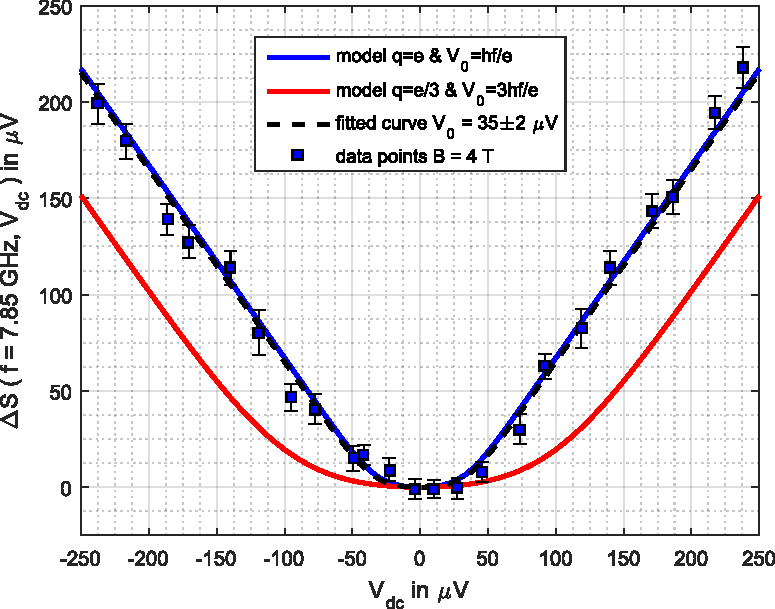
\includegraphics[width = 6.5 cm]{./chap2/nu_2_RF_noise_vs_Vdc_at_7_85GHz} &
			& 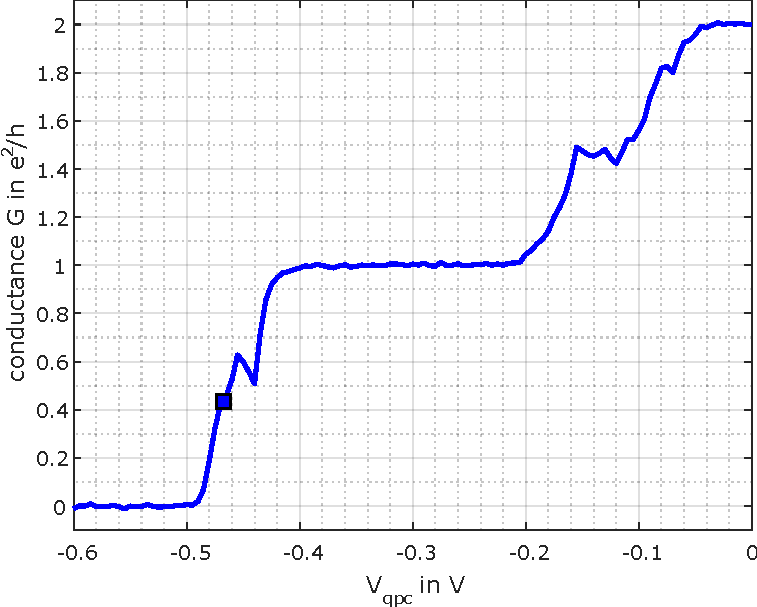
\includegraphics[width = 6.25 cm]{./chap2/qpc_step_nu_2}
		\end{tabular}
	\end{center}
	
	\caption{\textbf{High frequency noise measurement at integer filling factor $\nu = 2$.} \textbf{(a)} Data blue square points are measured at a frequency of 7.85 GHz as a function of bias voltage. The data points are consistent with the model of charge $q = e$ in blue line. The model of charge $q = \frac{e}{3}$ in red line is well separated from data points. The dashed line is the result of the model with the threshold voltage of noise emission $V_{0}$ let as a free fitting parameter. \textbf{(b)} Conductance measurement as a function of gate voltage $V_{\mathrm{qpc}}$ at zero bias $V_{\mathrm{dc}} = 0$ V. The two steps of the same amplitude of the blue line confirm the filling factor $\nu = 2$. The square point labels the gate voltage and transmission of the quantum point contact at which the high frequency noise is measured.}
	\label{fig: RF charac at 2}
\end{figure}

At the filling factor $\nu = 2$, the quantum point contact transmission is adjusted such that the inner edge-channel is totally reflected and the outer edge-channel is half transmitting.
%The local oscillator sets the measurement frequency at $f = 7.85$ GHz, in order that the no noise plateau without excess noise is larger in voltage than the thermal blurring with an electronic temperature $T_{\mathrm{elec}} = 50$ mK, $hf \gg k_{\mathrm{B}}T_{\mathrm{elec}}$.
The local oscillator sets the measurement frequency at $f = 7.85$ GHz, in order that the energy associated is bigger than the electronic temperature $hf \gg k_{\mathrm{B}}T_{\mathrm{elec}}$.
In the measurements of figure Fig. \ref{fig: RF charac at 2}, this implies that for low bias voltage $eV_{\mathrm{dc}} < hf$ neither the bias voltage nor the thermal excitations have enough energy to generate noise at frequency $f$, and the figure shows a plateau at $\Delta S\left(f,V_{\mathrm{dc}}\right) = 0$ $\upmu$V at low voltages.
%In measurements the rounding around the corners between the no noise plateau and the noise linear increase is dominated by the frequency bandwidth chosen with a cut-off frequency of low pass-filter at $\Delta f = 1.5$ GHz, because it correspond to a bigger energy than the temperature $h\Delta f > k_{\mathrm{B}}T_{\mathrm{elec}}$.
The frequency bandwidth is chosen with a cut-off frequency of low pass-filter at $\Delta f = 1.5$ GHz, as it corresponds to a bigger energy than the temperature $h\Delta f > k_{\mathrm{B}}T_{\mathrm{elec}}$ , it determines the rounding between the noise plateau at $\Delta S\left(f,V_{\mathrm{dc}}\right) = 0$ $\upmu$V and the linear increase of the noise.
The DC voltage applied belongs to a 200 $\upmu$V range, which is much greater than the expected threshold voltage $\frac{hf}{e} = 32 \upmu$V.
For voltages above this threshold data points plotted as blue squares in figure Fig. \ref{fig: RF charac at 2}, follow a linear curve.
The values of the noise are given by the voltages read at the lock-in amplifier, and in the figures the measurements are divided by one gain for each curves such that the slope of the linear part are $\pm1$ so $\Delta S \left(f,V_{\mathrm{dc}}\right) = \left|V_{\mathrm{dc}} \pm V_{0}\right|$ and the noise is expressed in $\upmu$V.
On the same graph Fig. \ref{fig: RF charac at 2} is plotted in blue line the expected curve for a non-interacting model \cite{blanter2000shot,martin2005course} of charge $e$, with an effective temperature $T_{\mathrm{elec}}$ due to the measurement bandwidth.
This model is expressed by the equation \eqref{eq: RF noise charge e}.

\begin{equation}
\Delta S \left(f,V_{\mathrm{dc}}\right) = \frac{1}{2}\left(V_{\mathrm{dc}}+\frac{hf}{q}\right)\coth\left(\frac{qV_{\mathrm{dc}}+hf}{2k_{\mathrm{B}}T_{\mathrm{elec}}}\right)+\frac{1}{2}\left(V_{\mathrm{dc}}-\frac{hf}{q}\right)\coth\left(\frac{qV_{\mathrm{dc}}-hf}{2k_{\mathrm{B}}T_{\mathrm{elec}}}\right)-\frac{hf}{q}\coth\left(\frac{hf}{2k_{\mathrm{B}}T_{\mathrm{elec}}}\right) \label{eq: RF noise charge e}
\end{equation}

with $q = e$.
The measured data points are consistent with this model. For the same non-interacting model with a fractional charge $e^{\star} = \frac{e}{3}$, the equation \eqref{eq: RF noise charge e} is unchanged except for the charge $q$ which is replaced by the fractional charge $e^{\star}$.
The red line plotted on the figure is given by this model with a fractional charge.
The data points with the sizes of their errobars allow excluding this last model, which demonstrates the ability of the technique to distinguish between situations with charge $e$ and $e^{\star}$.
The parameter which differentiates in this measurement the two models is the threshold voltage between the regime where the excess noise is constant at zero and its linear dependence as a function of voltage.
This threshold voltage, noted $V_{0}$, is linked to the excitation charges $q$ by the equation \eqref{eq: Josephson relation}, called the Josephson relation because it is the same equation as in a superconducting Josephson junction.

\begin{equation}
V_{0} = \frac{hf}{q} \label{eq: Josephson relation}
\end{equation}

To determine the measured value of $V_{0}$, the data points are fitted by the equation \eqref{eq: fit RF noise} with the parameter $V_{0}$ let as a free parameter.

\begin{equation}
\Delta S \left(f,V_{\mathrm{dc}}\right) = \frac{1}{2}\left(V_{\mathrm{dc}}+V_{0}\right)\coth\left(q\frac{V_{\mathrm{dc}}+V_{0}}{2k_{\mathrm{B}}T_{\mathrm{elec}}}\right)+\frac{1}{2}\left(V_{\mathrm{dc}}-V_{0}\right)\coth\left(q\frac{V_{\mathrm{dc}}-V_{0}}{2k_{\mathrm{B}}T_{\mathrm{elec}}}\right)-V_{0}\coth\left(\frac{qV_{0}}{2k_{\mathrm{B}}T_{\mathrm{elec}}}\right) \label{eq: fit RF noise}
\end{equation}

The resulting trace from this fitting procedure is represented as dashed black line in figure Fig. \ref{fig: RF charac at 2} and gives a value of $V_{0} = 35 \pm 2$ $\upmu$V.

\subsubsection*{Measurements for different frequencies at $\nu=3$.}

\begin{figure}[hptb]
	\begin{center}
		\begin{tabular}{c c c c}
			(a) & & (b) & \\
			& 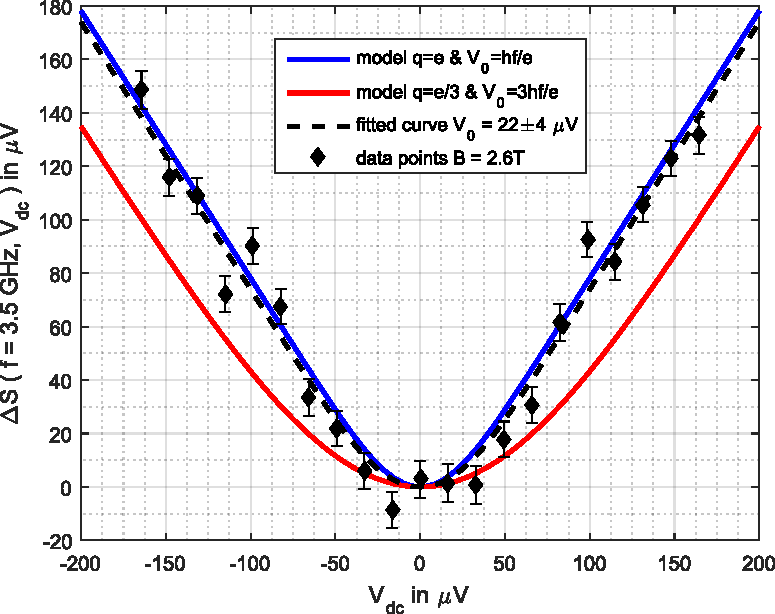
\includegraphics[width = 6.5 cm]{./chap2/nu_3_RF_noise_vs_Vdc_at_3_5GHz} &
			& 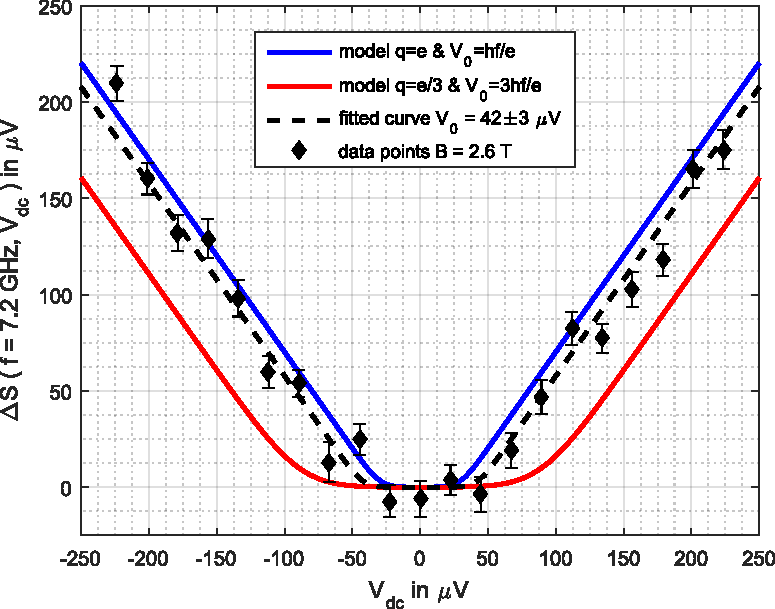
\includegraphics[width = 6.5 cm]{./chap2/nu_3_RF_noise_vs_Vdc_at_7_2GHz} \\
			(c) & & (d) & \\
			& 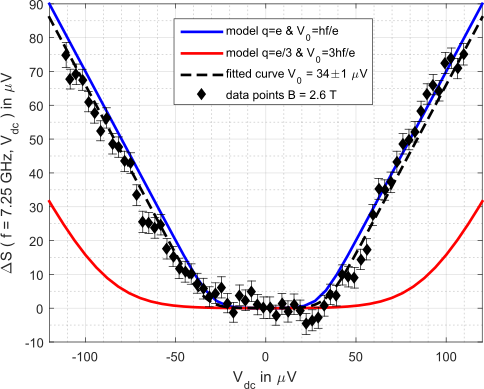
\includegraphics[width = 6.5 cm]{./chap2/nu_3_RF_noise_vs_Vdc_at_7_25GHz} &
			& 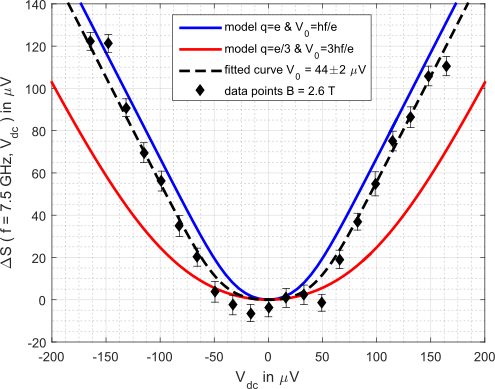
\includegraphics[width = 6.5 cm]{./chap2/nu_3_RF_noise_vs_Vdc_at_7_5GHz} \\
			(e) & & (f) & \\
			& 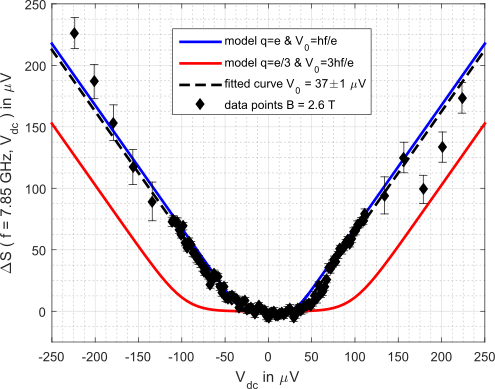
\includegraphics[width = 6.5 cm]{./chap2/nu_3_RF_noise_vs_Vdc_at_7_85GHz} &
			& 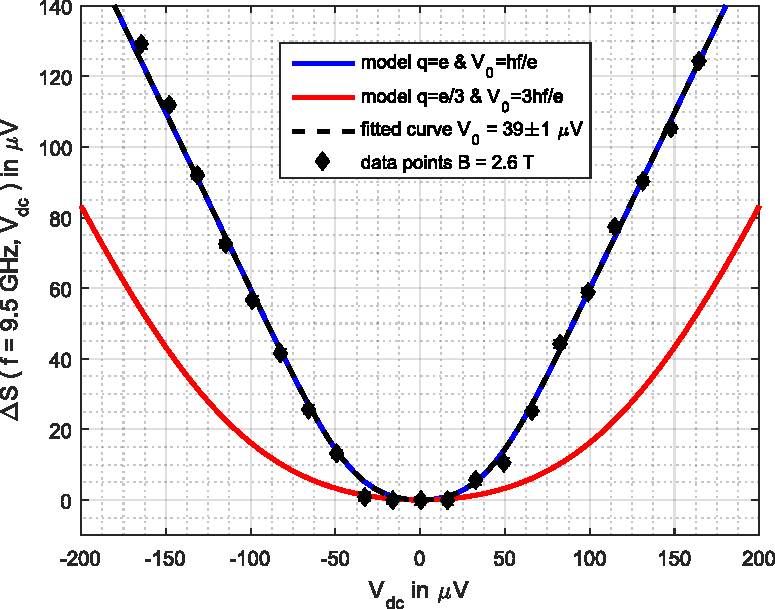
\includegraphics[width = 6.5 cm]{./chap2/nu_3_RF_noise_vs_Vdc_at_9_5GHz}
		\end{tabular}
	\end{center}
	
	\caption{\textbf{High frequency noise measurement for frequencies between $f = 3.5$ GHz and $f = 9.5$ GHz at filling factor $\nu = 3$.} The data points are plotted in black diamonds for this filling factor. For all curves integer charge $q = e$ models are still in blue lines, fractional charge models are still in red lines, and fitted lines in dashed lines. The data points and fitted curves agree with the model $q=e$ in all panels. The different parameter between panels is the increasing of the measurement frequency $f$ with \textbf{(a)} $f = 3.5$ GHz \textbf{(b)} $f = 7.2$ GHz \textbf{(c)} $f = 7.25$ GHz \textbf{(d)} $f = 7.5$ GHz \textbf{(e)} $f = 7.85$ GHz \textbf{(f)} $f = 9.5$ GHz.}
	\label{fig: RF charac at 3}
\end{figure}

In the relation \eqref{eq: Josephson relation}, $V_{0}$ remains constant between filling factors $\nu = 2$ and $\nu = 3$, because the current is still carried by electrons of charge $q = e$.
The other term is the frequency $f$ at which one measure the noise $\Delta S \left(f,V_{\mathrm{dc}}\right)$.
In this paragraph, we choose a filling factor $\nu = 3$ by applying a magnetic field $B = 2.6$ T, and the frequency $f$ has been changed first at $f = 3.5$ GHz, then around $f = 7.5$ GHz, finally at $f = 9.5$ GHz.
The measurement results are displayed in figure Fig. \ref{fig: RF charac at 3} with one panel for each frequency.
The data points at $\nu = 3$ are plotted in black diamonds, and the colour codes are conserved for the models, with blue lines corresponding to equation \eqref{eq: RF noise charge e}, red lines to the same equation with fractional charge $q = e^{\star}$, and dashed lines to a fit with the parameter $V_{0}$.
Among the different panels the range of the $V_{\mathrm{dc}}$ values change because as explained in the section \ref{sec: Experimental set-up chap2}, the voltage divider used to applied $V_{\mathrm{dc}}$ is changed.
The round shape at the threshold voltage $V_{0}$ has also not the same width between the graphs, because the bandwidth of noise integration varies by the changes of the low-pass filters, this is taken into account by selecting the correspondent $T_{\mathrm{elec}}$ in the models. 
The values of noise $\Delta S \left(f,V_{\mathrm{dc}}\right)$ are still divided by their slopes in the linear part of each curve, so they are expressed in $\upmu$V with a gain of 1.
On all panels the data points are close to the blue line of charge $q = e$ in comparison with their error-bars, and they are far from the red line of charge $q = e^{\star}$.
In the same way the fitted curve in dashed line is much closer to the blue than the red line, so the current is still carried by electrons at $\nu = 3$.
The results $V_{0}$ from the fits of each graph increase with frequency overall measurements from $V_{0} = 22 \pm 4$ $\upmu$V at $f = 3.5$ GHz in the panel (a) to $V_{0} = 39 \pm 1$ $\upmu$V at $f = 9.5$ GHz in the panel (f).
This increase is consistent with the frequency dependence of relation \eqref{eq: Josephson relation}, where the threshold voltage is proportional to the frequency $f$.

\subsection{Fractional quantum Hall effect regime}

The experimental method has been validated with the above measurement in the integer quantum Hall regime, so it can be used to investigate the fractional quantum Hall regime.

\subsubsection*{First fractional charges measurement at $\nu = \frac{2}{3}$.}

The first technique to reach the fractional regime is to increase the magnetic field until the filling factor of the sample is fractional.
In the following results the filling factor at which we stop is $\nu = \frac{2}{3}$ at a magnetic field of $B = 12$ T.
We did not reach $\nu = \frac{1}{3}$, which is a better defined fractional state, because it would have required, with the used samples of charge carrier density of $n = \nu\frac{eB}{h} \sim 2.10^{11}$ cm$^{-2}$, to apply a twice stronger magnetic field of $B = 24$ T well above the capacity of our system.

\paragraph*{Low frequency characterization.}

\begin{figure}[hptb]
	\begin{center}
		\begin{tabular}{c c c c}
			(a) & & (b) & \\
			& 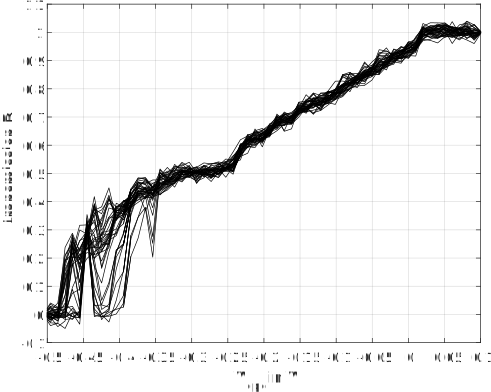
\includegraphics[width = 6.5 cm]{./chap2/nu_2_3_D_vs_Vqpc_for_several_Vdc} &
			& 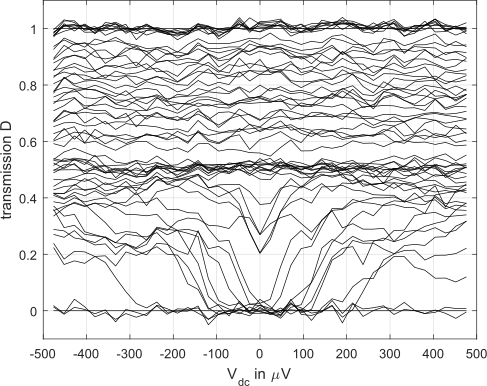
\includegraphics[width = 6.5 cm]{./chap2/nu_2_3_D_vs_Vdc_for_several_Vqpc} \\
			(c) & & (d) & \\
			& 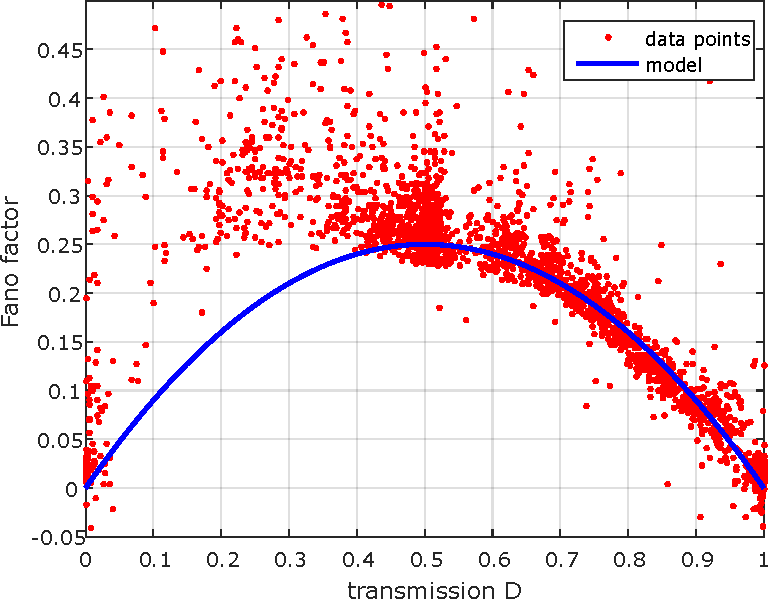
\includegraphics[width = 6.5 cm]{./chap2/nu_2_3_noise_vs_D_for_several_Vdc} &
			& 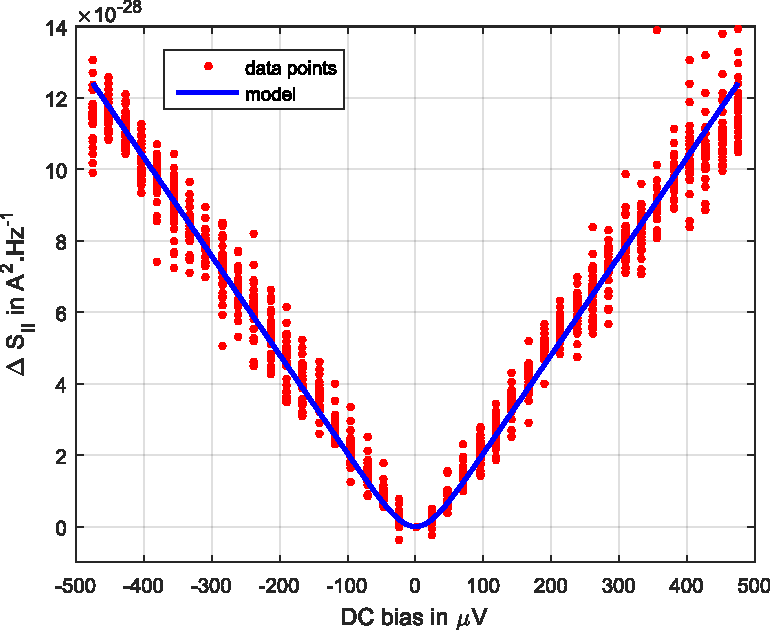
\includegraphics[width = 6.5 cm]{./chap2/nu_2_3_noise_vs_Vdc_for_D_0_4_0_9}
			
		\end{tabular}
	\end{center}
	
	\caption{\textbf{Conductance and low frequency noise measurement at fractional filling factor $\nu = \frac{2}{3}$.} Panels (a) and (b) are conductance measurements as a function of gate voltages $V_{\mathrm{qpc}}$ and bias voltage $V_{\mathrm{dc}}$. The transmission $D$ is proportional to the conductance $G$ by a factor $G = \frac{2e^{2}}{3h}D$. In the panel \textbf{(a)}, the transmission is plotted as a function of $V_{\mathrm{qpc}}$ and shows plateaus at $D = 0$, $0.5$, $1$. In the panel \textbf{(b)}, the transmission is plotted as a function of $V_{\mathrm{dc}}$ and displays flat line in weak backscattering regime. Panels (c) and (d) are related to low frequency noise measurements. In the panel \textbf{(c)}, the plotted variable is the Fano factor computed by the low frequency noise divided by right terms of equation \eqref{eq: bruit BF nu=2/3} without the $D\left(1-D\right)$ term. Red points are deduced from measured values of low frequency noise for each bias voltage $V_{\mathrm{dc}}$ and gate voltages $V_{\mathrm{qpc}}$ plotted as a function of the measured transmission $D$ in above panels. The blue line is the parabola $D\left(1-D\right)$ given by the model of equation \eqref{eq: bruit BF nu=2/3}. In the panel \textbf{(d)}, the same measurement red points are plotted but the noise is divided by $D\left(1-D\right)$ with $D$ the measured transmission and only for values of $D \geq 0.5$. The blue line is the model of \eqref{eq: bruit BF nu=2/3}.}
	\label{fig: LF charac at 2/3}
\end{figure}

The first characterization is to measure the conductance of the quantum point contact at a magnetic field of $B = 12$ T, as a function of the two applied voltages $V_{\mathrm{dc}}$ and $V_{\mathrm{qpc}}$.
In figure Fig. \ref{fig: LF charac at 2/3} panels (a) and (b), the measurements of conductance are plotted.
In the two parameters, the bias voltage $V_{\mathrm{dc}}$ shifts the chemical potential of one input edge channel versus the opposite input edge channel. 
By varying this parameter we can check if the conductance varies with the bias voltage, for the characterization $V_{\mathrm{dc}}$ is varied in the $\pm$500 $\upmu$V maximum range of the high frequency noise measurements.
The other parameter, the voltage applied to quantum point contact gates $V_{\mathrm{qpc}}$ is varied towards negative voltages until the conductance reaches the plateau of a completely close quantum point contact, it happens for $V_{\mathrm{qpc}} < -0.5$ V.
The gate voltage $V_{\mathrm{qpc}}$ is also varied towards the positive voltages until it reaches the plateau of a completely open quantum point contact, it occurs for $V_{\mathrm{qpc}} > 0.05$ V.
The conductance is plotted as the transmission $D = \frac{3h}{2e^{2}}G$ included between 0 for closed and 1 for open quantum point contact.
The panel (a) of figure Fig. \ref{fig: LF charac at 2/3} represents the transmission $D$ as a function of the gates voltage $V_{\mathrm{qpc}}$, where each line corresponds to one bias voltage $V_{\mathrm{dc}}$.
The lines form plateaus at transmissions 0 and 1, which are a conductance $G$ of 0 and $\frac{2e^{2}}{3h}$, and also at transmission 0.5, so at a conductance $G = \frac{e^{2}}{3h}$.
In the panel (b), the role of $V_{\mathrm{qpc}}$ and $V_{\mathrm{dc}}$ are exchanged, and the transmission $D$ is plotted in function of $V_{\mathrm{dc}}$, with one line corresponding to each value of $V_{\mathrm{qpc}}$.
On this panel the lines accumulate and make a bold line at transmission 0, 0.5 and 1, showing the conductance plateaus of the panel (a) at conductances 0, $\frac{e^{2}}{3h}$, and $\frac{2e^{2}}{3h}$.
The system is then in a regime where the conductance is quantized in fractions of the quantum of conductance $\frac{e^{2}}{h}$.
At the same time, the low frequency shot noise has been recorded as a function of $V_{\mathrm{qpc}}$ and $V_{\mathrm{dc}}$.
These measurements correspond to panels (c) and (d) of figure Fig. \ref{fig: LF charac at 2/3}.
The low frequency noise measurement has already been used to measure the charge of fractional excitations in \cite{saminadayar1997observation,de1998direct,reznikov1999observation,hashisaka2015shot}, here we reproduce the same experiment to characterize the system.
The excess low frequency noise is related to the charge thanks the equation \eqref{eq: bruit BF nu=2/3}, with a model of a quantum point contact as a tunnel barrier of transmission $D$ partitioning a channel of total conductance $G=\frac{2e^{2}}{3h}$, with a voltage difference of $V_{\mathrm{dc}}$ between the two inputs at temperature $T_{\mathrm{elec}} = 40$ mK, and tunnelling particles of charge $q$. 

\begin{equation}
\Delta S\left(f=0,V_{\mathrm{dc}}\right) = 4D\left(1-D\right)\frac{2e^{2}}{3h}k_{\mathrm{B}}T_{\mathrm{elec}}\left(\frac{qV_{\mathrm{dc}}}{2k_{\mathrm{B}}T_{\mathrm{elec}}}\coth\left(\frac{qV_{\mathrm{dc}}}{2k_{\mathrm{B}}T_{\mathrm{elec}}}\right)-1\right) \label{eq: bruit BF nu=2/3}
\end{equation}

%The model chosen is of Laughlin particles \cite{laughlin1983anomalous} tunnelling of charge $q = e^{\star} = \frac{e}{3}$, in panel (c) the dependence in transmission $D$ is checked, and in panel (d) it is the variation as a function of voltage $V_{\mathrm{dc}}$.
The model chosen is one channel of transmission $D$ and of charge tunnelling is $q = e^{\star} = \frac{e}{3}$ like Laughlin particles \cite{laughlin1983anomalous}, the resulting dependence of the noise on $D$ is checked in the panel (c) and the variation of the noise as a function of $V_{\mathrm{dc}}$ is verified in the panel (d).
In the panel (c) each data point in red measured for a couple of parameters $V_{\mathrm{dc}}$ and $V_{\mathrm{qpc}}$ are plotted at the abscissa of the transmission $D$ measured in above panels, and the y-axis is the measured noise $\Delta S\left(f=0,V_{\mathrm{dc}}\right)$ divided by the modelled bias voltage contribution $4\frac{2e^{2}}{3h}k_{\mathrm{B}}T_{\mathrm{elec}}\left(\frac{qV_{\mathrm{dc}}}{2k_{\mathrm{B}}T_{\mathrm{elec}}}\coth\left(\frac{qV_{\mathrm{dc}}}{2k_{\mathrm{B}}T_{\mathrm{elec}}}\right)-1\right)\underset{T_{\mathrm{elec}}\to0}{\longrightarrow}2qI$, with $q = \frac{e}{3}$, this quotient is the Fano factor.
In blue is plotted the Fano factor expected from the model, which is the parabola $D\left(1-D\right)$.
The data points in the panel (c) are distributed on a single parabola which is the result of a model with a single channel of conductance $\frac{2e^{2}}{3h}$.
The panel (c) also shows that the model is consistent with the measurement only for transmission above 0.4.
This agrees that on the panel (b) only lines of transmission above 0.4 are flat, so only above this number the transmission does not depend on the bias voltage $V_{\mathrm{dc}}$.
In the panel (d), only points of transmission above 0.4 are selected, to check their $V_{\mathrm{dc}}$ dependence.
The data points are the measured noise divided by the Fano factor $D\left(1-D\right)$ with $D$ the measured transmission plotted as a function of $V_{\mathrm{dc}}$ for all values of the gate voltage $V_{\mathrm{qpc}}$.
The model prediction plotted in blue line is given by the equation \eqref{eq: bruit BF nu=2/3} divided by the Fano factor $D\left(1-D\right)$ for the charge $q = e^{\star} = \frac{e}{3}$.
As already shown by the panel (c), model and measure are consistent.
This last panel is the usual graph displayed in articles \cite{saminadayar1997observation,de1998direct,reznikov1999observation} to get the value of the fractional charges.
Surprisingly, these results differ from some previous measurements in \cite{bid2009shot,kapfer2018dynamic}, where they measure a fractional charge of $q=\frac{2e}{3}$ at a temperature $T_{\mathrm{elec}} = 40$ mK but if the temperature is increased up to $T_{\mathrm{elec}} = 120$ mK or if the shot noise is measured thanks to cross-correlation of the current between the two output edge-channels of the qpc, then a fractional charge of $q=\frac{e}{3}$ is found again.
To perform the high frequency noise measurements we chose to set the transmission at $D = 0.8$ in the weak-backscattering regime, where low frequency shot noise measurement gives a fractional charge of $q=\frac{e}{3}$.

\paragraph*{High frequency measurements.}

\begin{figure}[hptb]
	\begin{center}
		\begin{tabular}{c c c c}
			(a) & & (b) & \\
			& 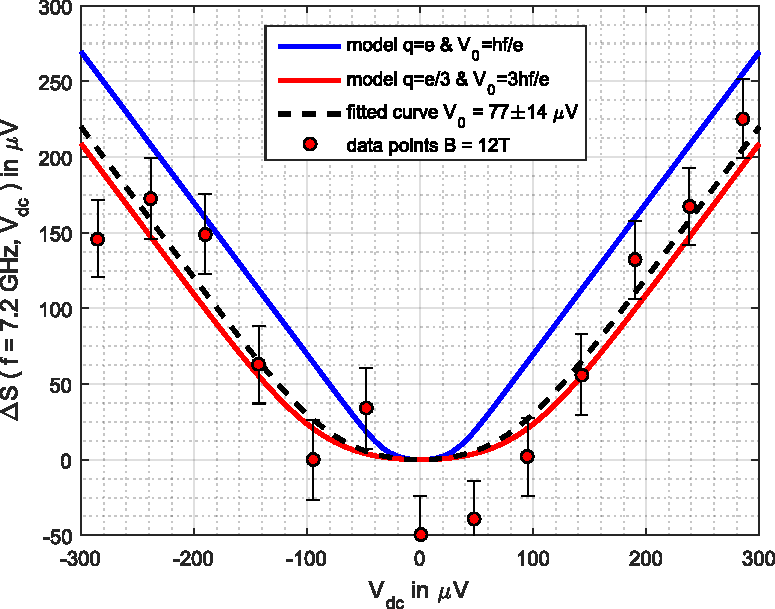
\includegraphics[width = 6.5 cm]{./chap2/nu_2_3_RF_noise_vs_Vdc_at_7_2GHz} &
			& 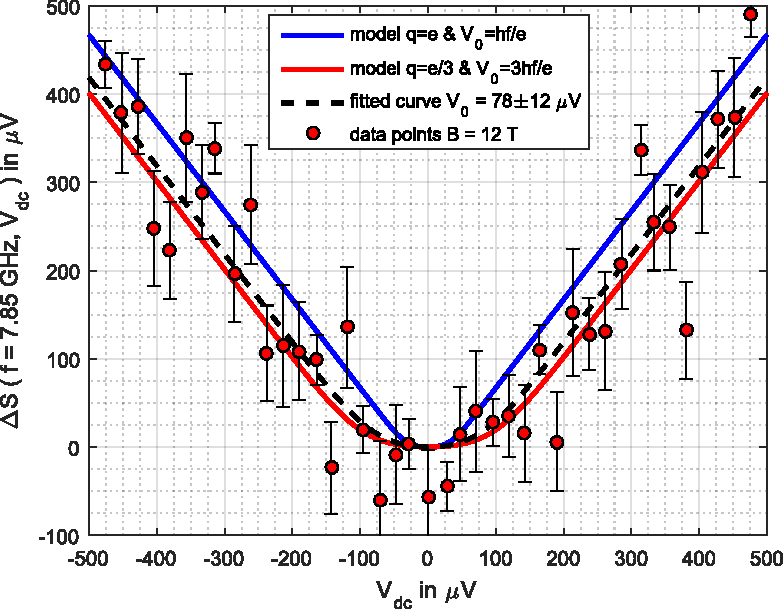
\includegraphics[width = 6.5 cm]{./chap2/nu_2_3_RF_noise_vs_Vdc_at_7_85GHz}
			
		\end{tabular}
	\end{center}
	
	\caption{\textbf{High frequency noise measurement at fractional filling factor $\nu = \frac{2}{3}$.} \textbf{(a)} Few red circle points are measured to show they are closer to the model of fractional charge $q = \frac{e}{3}$ in red line than the blue line corresponding to $q = e$. \textbf{(b)} More points are measured in a wider range of bias voltage $V_{\mathrm{dc}}$. Single points do not allow to distinguish between $q = e$ and $q = \frac{e}{3}$ model, but the dashed fitted line is closer to the $q = \frac{e}{3}$ model.}
	\label{fig: RF charac at 2/3}
\end{figure}

The high frequency measurements are divided in two data sets, which are the two panels of figure Fig. \ref{fig: RF charac at 2/3}.
The axes, which are the noise $\Delta S$ in $\upmu$V as a function of $V_{\mathrm{dc}}$ in $\upmu$V, are the same as in previous results for high frequency noise, and also the represented elements are identical with data points plotted in red circles, models in lines, and fit in dashed lines.
In the panel (a), the measurement is performed at a frequency $f = 7.2$ GHz, with few points, in a medium range of $\pm300 \upmu$V, whereas in the panel (b) the measurement is performed at a close frequency $f = 7.85$ GHz, in a larger range of $\pm500 \upmu$V, with more points.
First one remarks that the error-bars of data points are much bigger than for last subsection results in the integer quantum Hall regime.
This reduction of the measurement sensitivity is due to the decrease of the gain of the measurement line with the magnetic field.
It can have two origins, the increasing impedance mismatch between the sample resistance, which is proportional to the magnetic field, and the lines 50 $\Omega$ impedance, and the increase of noise attenuation in the propagation between the quantum point contact and the output Ohmic contact.
Due to this bigger error-bars, when a lot of points are measured in the panel (b), it is not clear for each single point to determine if they agree with a model of charge $q = e$ or $q = e^{\star} = \frac{e}{3}$.
In the panel (a), with fewer points, the error bars are small enough to have data points consistent with the model \ref{eq: RF noise charge e} with charge $q = \frac{e}{3}$ in red line, and not with charge $q = e$ in blue line.
The fit enables to take into account all points together in the determination of the threshold voltage $V_{0}$, the results in the panel (a) as seen from each individual point show a dashed line close to the model $q = \frac{e}{3}$, and in the panel (b) it enables to conclude because it also gives a dashed line close to the model $q = \frac{e}{3}$.
These measurements by the following equation \ref{eq: RF noise charge e} indicate that in this fractional regime results are the same as in the integer regime with just the elementary charge replaced by fractional one.
In the integer case the absence of noise, meaning the absence of microwave photons emitted at the energy $hf$, when the voltage difference between the two input edge-channels is below the threshold $V_{0} = \frac{hf}{q}$, is due to the Pauli's exclusion principle and the Fermionic statistics of electrons.
Indeed only electrons at energies between the Fermi level of the opposite edge-channel and $eV_{\mathrm{dc}}$ above it, can tunnel through the quantum point contact because other states are fully occupied, so the generated out-of-equilibrium state as a maximum of available energy of $eV_{\mathrm{dc}}$ to generate microwave photons of quantized energy $hf$.
For elementary particles of fractional charge $\frac{e}{3}$ introduced by Laughlin \cite{laughlin1983anomalous}, the expected statistic is an anyonic statistic and not a Fermionic statistic, so the experiment seems to confirm the work \cite{haldane1991fractional} suggesting that there may be an effect analogue to Pauli's exclusion principle for fractional charges.

This experiment has been preceded by several theoretical proposals \cite{crepieux2004photoassisted,ferraro2014multiple,carrega2014finite,carrega2012spectral} aiming at computing the finite frequency shot noise through a tunnel barrier in presence of fractionally charged particles.
%In these works the expected shape of the finite frequency noise present peaks as a function of bias voltage that are not seen in this experiment.
In these works the noise plateau is predicted for voltages $V_{\mathrm{dc}}$ close to zero.
This plateau stops and the noise presents some variation as predicted when the introduced characteristic frequency $f_{J} = \frac{qV_{\mathrm{dc}}}{h}$, with $q$ the fractional charge, is equal to the noise measurement frequency $f$.
Their calculations are based on a Tomonaga-Luttinger liquid model from which all quantities conductance, zero frequency shot noise and finite frequency shot noise are evaluated.
This precise model leads to the presence of noise peaks as a function of $V_{\mathrm{dc}}$ at $f_{J} = f$, which are not observed in this experiment.
Without assuming a Tomonaga-Luttinger liquid model, and without evaluating the conductance and the low frequency shot noise, theoretical calculations \cite{roussel2016perturbative} in the weak-backscattering regime link the conductance and the zero frequency shot noise to finite frequency shot noise.
This correspondence between the finite frequency and zero frequency measurements is only determined by the comparison between the measurement frequency $f$ and the characteristic frequency $f_{J}$.
In the experimental conditions, this link is approximate by equation \eqref{eq: link shot noise 0 and f}.

\begin{equation}
\Delta S\left(f,V_{\mathrm{dc}}\right) = \frac{1}{2}\left(\Delta S\left(0,V_{\mathrm{dc}}-\frac{hf}{q}\right)+\Delta S\left(0,V_{\mathrm{dc}}+\frac{hf}{q}\right)\right) \label{eq: link shot noise 0 and f}
\end{equation}

Since for the chosen transmission $D = 0.8$ the conductance is constant with bias voltage, see panel (b) figure Fig. \ref{fig: LF charac at 2/3}, the zero frequency shot noise is given by equation \eqref{eq: bruit BF nu=2/3}, see panel (d) figure Fig. \ref{fig: LF charac at 2/3}, the finite frequency noise deduced by equations \eqref{eq: bruit BF nu=2/3} and \eqref{eq: link shot noise 0 and f} is given by \eqref{eq: RF noise charge e} , see figure Fig. \ref{fig: RF charac at 2/3}.

\subsubsection*{Noise frequency dependence studied with fractional charges at filling factor $\nu = \frac{4}{3}$}

To study the frequency dependence in the fractional quantum Hall effect, we need to perform more measurements at different frequencies.
As at $\nu = \frac{2}{3}$ the measurement gain is low, the other technique to reach the fractional quantum Hall regime is to adjust the magnetic field for a fractional filling factor above 1.
The chosen filling factor is $\nu = \frac{4}{3}$ reached at $B = 5.7$ T, at this filling factor the measurement gain increase compared to $\nu = \frac{2}{3}$ and the high frequency noise measurement can be repeated for several frequencies from 3.5 GHz to 8 GHz.

\paragraph*{Low frequency characterization.}

\begin{figure}[hptb]
	\begin{center}
		\begin{tabular}{c c c c}
			(a) & & (b) & \\
			& 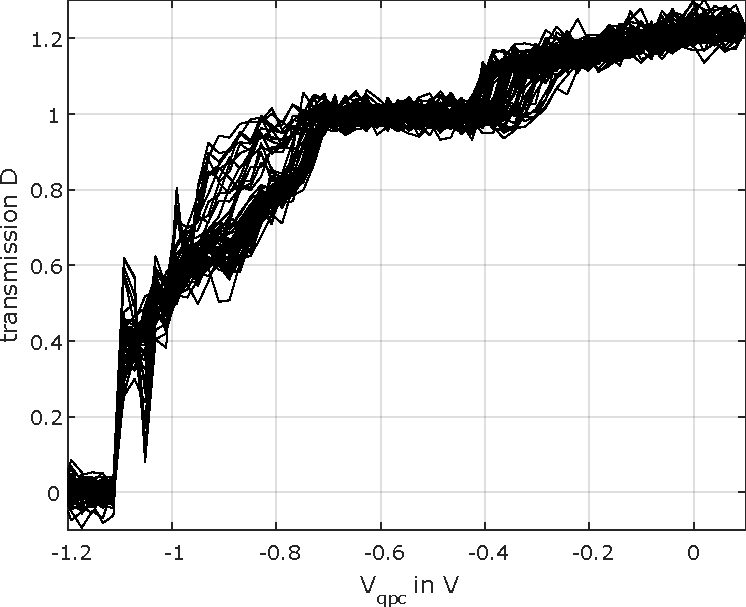
\includegraphics[width = 6.5 cm]{./chap2/nu_4_3_D_vs_Vqpc_for_several_Vdc} &
			& 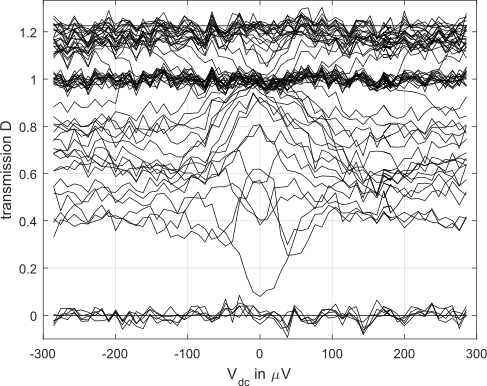
\includegraphics[width = 6.5 cm]{./chap2/nu_4_3_D_vs_Vdc_for_several_Vqpc} \\
			(c) & & (d) & \\
			& \includegraphics[width = 6.5 cm]{./chap2/nu_4_3_noise_vs_D_for_several_Vdc} &
			& 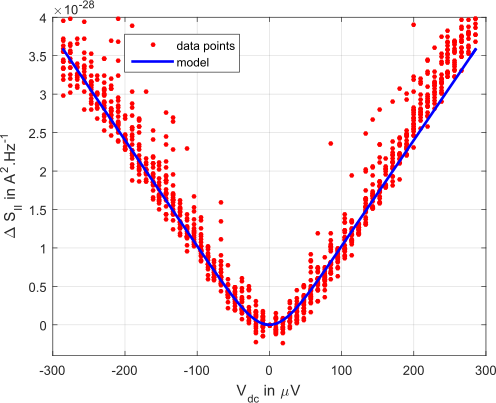
\includegraphics[width = 6.5 cm]{./chap2/nu_4_3_noise_vs_Vdc_for_D_1_15_1_3}
		\end{tabular}
	\end{center}
	
	\caption{\textbf{Conductance and low frequency noise measurement at fractional filling factor $\nu = \frac{4}{3}$.} In this figure the same measures as in figure Fig. \ref{fig: LF charac at 2/3} are plotted. \textbf{(a)} The measurements at different bias voltage of transmission versus gate voltage $V_{\mathrm{qpc}}$ show one step at a conductance of $G = \frac{e^{2}}{h}$ labelled as transmission $D = 1$ and the second step is not fully measured as it saturates before a conductance of $G = \frac{e^{2}}{h}+\frac{e^{2}}{3h}$ corresponding to a transmission of $D = 1+\frac{1}{3}$. \textbf{(b)} The same measurement plotted as a function of the bias voltage show an accumulation of line at the plateau location of transmission 1, and only at a transmission $D = 1.2$ the transmission is independent of $V_{\mathrm{dc}}$, so it is the transmission chosen for the high frequency noise measurement. \textbf{(c)} The noise measurement as a function of the transmission shows two parabolas corresponding to the two equations \eqref{eq: bruit BF nu=4/3}. These two parabolas can be interpreted by the partitioning of two edge-channels of conductance $G = \frac{e^{2}}{h}$ and $G = \frac{e^{2}}{3h}$, and carrying charge $q = e$ and $q = \frac{e}{3}$. \textbf{(d)} Only points at a transmission $D \geq 1.15$ are selected in this graph where the noise is plotted as a function of bias voltage. The blue line is given by the second equation of \eqref{eq: bruit BF nu=4/3} which confirms the model of charge $q = \frac{e}{3}$.
	%The transmission is set at $D = 1.2$ for high frequency noise measurement where the low frequency noise measurement agrees with the blue line model.
	}
	\label{fig: LF charac at 4/3}
\end{figure}

The low frequency measurements in figure Fig. \ref{fig: LF charac at 4/3} show the presence of fractional charges at filling factor $\nu = \frac{4}{3}$.
As previously the panels (a) and (b) display the conductance measurements as a function of gate and bias voltages $V_{\mathrm{qpc}}$ and $V_{\mathrm{dc}}$.
On the panel (a), the conductance shows one clear step at $-0.7$ V$\leq V_{\mathrm{qpc}}\leq -0.4$ V, which corresponds to a transmission $D = 1$, for more negative $V_{\mathrm{qpc}}\leq -1.2$ V the quantum point contact is closed $D = 0$, for more positive value the quantum point contact is not completely open and the transmission saturates at 1.25 before $\frac{4}{3}$.
On the panel (b), the darker zone at $D = 1$ confirms the conductance plateau, the other accumulation of lines around  $D = 1.2$ agrees with saturation of the transmission before the complete opening of the quantum point contact.
The panel (c) still plots the Fano factor defined here as the low frequency noise $\Delta S\left(f=0,V_{\mathrm{dc}}\right)$ divided by $4\frac{e^{2}}{h}k_{\mathrm{B}}T_{\mathrm{elec}}\left(\frac{eV_{\mathrm{dc}}}{2k_{\mathrm{B}}T_{\mathrm{elec}}}\coth\left(\frac{eV_{\mathrm{dc}}}{2k_{\mathrm{B}}T_{\mathrm{elec}}}\right)-1\right)$.
The measured points in red points are consistent with a model in blue line showing a double parabola shape.
This model is based on two edge channels, for transmission $0 \leq D \leq 1$ one edge channel of conductance $\frac{e^{2}}{h}$ and carrying charges $q = e$ is partitioned, for transmission $0 \leq D^{\star} \leq 1$, with $D^{\star} = \frac{D-1}{3}$, the partitioned edge channel has a conductance $\frac{e^{2}}{3h}$ and carries charges $q = e^{\star} = \frac{e}{3}$.
The two parabolas are given by the two equations \eqref{eq: bruit BF nu=4/3}.

\begin{align}
\Delta S\left(f=0,V_{\mathrm{dc}}\right) &= 4D\left(1-D\right)\frac{e^{2}}{h}k_{\mathrm{B}}T_{\mathrm{elec}}\left(\frac{eV_{\mathrm{dc}}}{2k_{\mathrm{B}}T_{\mathrm{elec}}}\coth\left(\frac{eV_{\mathrm{dc}}}{2k_{\mathrm{B}}T_{\mathrm{elec}}}\right)-1\right) \\
\Delta S\left(f=0,V_{\mathrm{dc}}\right) &= 4D^{\star}\left(\frac{1}{3}-D^{\star}\right)\frac{e^{2}}{3h}k_{\mathrm{B}}T_{\mathrm{elec}}\left(\frac{e^{\star}V_{\mathrm{dc}}}{2k_{\mathrm{B}}T_{\mathrm{elec}}}\coth\left(\frac{e^{\star}V_{\mathrm{dc}}}{2k_{\mathrm{B}}T_{\mathrm{elec}}}\right)-1\right)
\label{eq: bruit BF nu=4/3}	
\end{align}

The smallest parabola indicates the presence of fractional charges, which we are interesting in. 
To confirm their presence the panel (d) plots the low frequency shot noise $\Delta S\left(f=0,V_{\mathrm{dc}}\right)$ divided by $D^{\star}\left(1-D^{\star}\right)$ for $0.5 \leq D^{\star}$ as a function of $V_{\mathrm{dc}}$.
As expected the measured red points agree with the blue line model given by the second equation of \eqref{eq: bruit BF nu=4/3}.
In this graph the charge is given by the slope of the noise, and one can remark that its slope is twice smaller than for the $\nu = \frac{2}{3}$ figure Fig. \ref{fig: LF charac at 2/3} panel (d), they have the same charge $q = e^{\star}$ but they have different conductance $\frac{2e^{2}}{3h}$ for $\nu = \frac{2}{3}$ and $\frac{e^{2}}{3h}$ for $\nu = \frac{4}{3}$.
The working point for high frequency measurements is chosen at a transmission $D = 1.2$ thanks to these measurements.

\paragraph*{High frequency measurements.}

\begin{figure}[hptb]
	\begin{center}
		\begin{tabular}{c c c c}
			(a) & & (b) & \\
			& 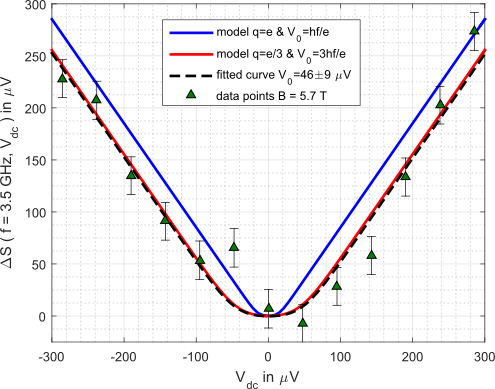
\includegraphics[width = 6.5 cm]{./chap2/nu_4_3_RF_noise_vs_Vdc_at_3_5GHz} &
			& 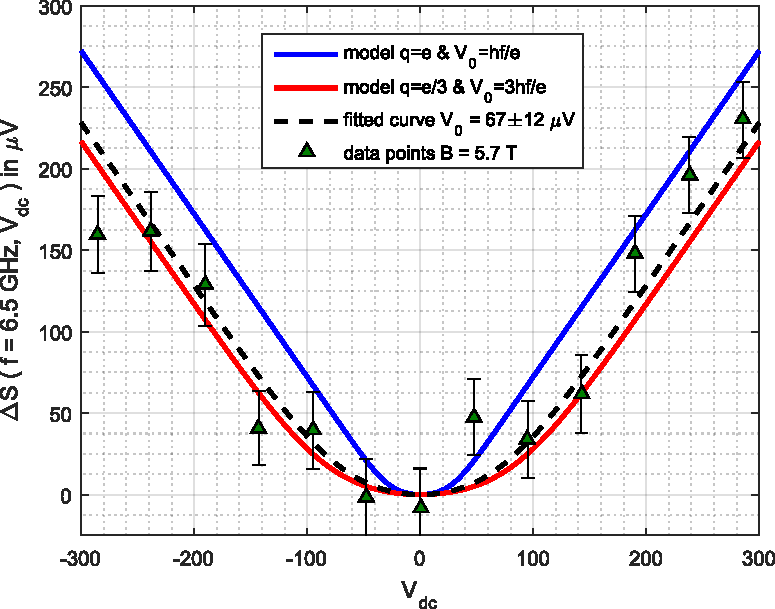
\includegraphics[width = 6.5 cm]{./chap2/nu_4_3_RF_noise_vs_Vdc_at_6_5GHz} \\
			(c) & & (d) & \\
			& \includegraphics[width = 6.5 cm]{./chap2/nu_4_3_RF_noise_vs_Vdc_at_6_75GHz} &
			& \includegraphics[width = 6.5 cm]{./chap2/nu_4_3_RF_noise_vs_Vdc_at_8GHz}
		\end{tabular}
	\end{center}
	
	\caption{\textbf{High frequency noise measurement for different frequencies between $f= 3.5$ GHz and $f = 8$ GHz at filling factor $\nu = \frac{4}{3}$.} Data points are green triangles for the filling factor $\nu = \frac{4}{3}$. For the chosen weak-backscattering regime data points in all panels and the fitted curve in dashed lines are consistent with the model $q = \frac{e}{3}$ in red line. Between different panels the measurement frequency $f$ is increased from $f = 3.5$ GHz in \textbf{(a)}, $f = 6.5$ GHz in \textbf{(b)}, $f = 6.75$ GHz in \textbf{(c)}, to $f = 8$ GHz in \textbf{(d)}.}
	\label{fig: RF charac at 4/3}
\end{figure}

Following the same method as above the high frequency noise is measured and plotted in green triangles in figure Fig. \ref{fig: RF charac at 4/3}.
The four panels are measurements at increasing frequency from 3.5 GHz to 8 GHz.
In each panel the blue line is the model \eqref{eq: RF noise charge e} with a charge $q = e$, the red line with a charge $q = \frac{e}{3}$, and the dashed line is the result of threshold voltage $V_{0}$ fit in equation \eqref{eq: fit RF noise}.
In the four panels data points and the fitted dashed lines are closer to the red line than the blue line.
From the high frequency noise, we can also conclude that excitations are carried by fractional charges at the transmission $D = 1.2$ and filling factor $\nu = \frac{4}{3}$.
This conclusion is valid for each panel, so for each frequency, and one can remark that the voltage threshold $V_{0}$ increases from  $46 \pm 9$ $\upmu$V at 3.5 GHz to $109 \pm 6$ $\upmu$V at 8 GHz.
With these measurements and the high frequency noise measurement at filling factor $\nu = 3$, there are two data sets, which allow to study the evolution of the high frequency noise with the measurement frequency.

\subsection{Frequency and charge dependence}

\begin{figure}[hptb]
	\begin{center}
		\begin{tabular}{c c c c}
			(a) & & (b) & \\
			& \includegraphics[width = 6.5 cm]{./chap2/V_0_vs_f_for_different_nu} &
			& \includegraphics[width = 6.5 cm]{./chap2/noise_vs_V_dc_for_different_nu}
		\end{tabular}
	\end{center}
	
	\caption{\textbf{Frequency and charge dependence of high frequency noise.} \textbf{(a)} The threshold voltage $V_{0}$ got from the fitting of experimental data is plotted as a function of the measurement frequency. The shape and the colour of points correspond to the same shape and colour for the filling factor of the measurement points. The red line is the threshold voltage given by a model of fractional charge $q = \frac{e}{3}$ in equation \eqref{eq: Josephson relation}. The blue line is the model for an integer charge $q = e$. Dashed lines are similar to plain lines with a frequency $f$ shifted by plus or minus the measurement bandwidth around $f$. \textbf{(b)} All high frequency noise measurements $\Delta S$ plotted as a function of the bias voltage $V_{\mathrm{dc}}$. Both noise and voltage are multiplied by the factor $\frac{q}{hf}$ with $f$ the measurement frequency and $q$ the measured charge $e$ or $\frac{e}{3}$ given in (a). All data are consistent with the same model \eqref{eq: RF noise charge e} in yellow dashed line.}
	\label{fig: charac for all nu}
\end{figure}

This subsection re-use all measurements at different filling factors and different frequencies to discuss the charge and frequency dependence of the high frequency noise.
The voltage threshold $V_{0}$ is the fitting parameter used to determine the charge in the different measurements, so it is the parameter that summarizes the high frequency noise measurement at one frequency and one filling factor.
The equation \eqref{eq: Josephson relation} relates the measured threshold voltage $V_{0}$ with the chosen measurement frequency $f$ and the excitations charge $q$.
The panel (a) of figure Fig. \ref{fig: charac for all nu} checks the agreement between measurements and relation \eqref{eq: Josephson relation}.
%The characteristic frequency associated with the threshold voltage $\frac{eV_{0}}{h}$ is plotted as a function of the measurement frequency $f$.
The threshold voltage $\frac{eV_{0}}{h}$ is plotted as a function of the measurement frequency $f$.
The data points have the same shape and colour as above associated with their filling factor: red circle for $\nu = \frac{2}{3}$, green triangles for $\nu = \frac{4}{3}$, blue squares for $\nu = 2$, black diamonds for $\nu = 3$.
The blue line is the equation \eqref{eq: Josephson relation} with integer charge $q = e$ and the red line with fractional charge $q = \frac{e}{3}$.
The data points at integer filling factors follow the trend of integer charge blue line, and the data points at fractional filling factor follow the trend of fractional charge red line.
To get a better agreement between data points and the models, one needs to consider that the high frequency noise is integrated on a bandwidth around the central frequency $f$.
This integration increases only the signal level and the effective electronic temperature $T_{\mathrm{elec}}$ when the band width increases if the noise measurement gain is flat with frequency.
This effect is already taken into account, but if the noise measurement gain is not flat with frequency there are more modifications of the noise measurement parameters.
With a gain that depends on frequency, the effective central frequency $f$ at which the noise is measured can be shifted inside the bandwidth $\Delta f$, so the dashed line are the models given by \eqref{eq: Josephson relation}, with a frequency $f$ replaced by $f\pm\frac{\Delta f}{\sqrt{3}}$.
The blue and red dashed lines are still well separate, this allows separating integer and fractional charges, and most of the data points error bars overlap the interval between the two dashed lines of either one model or the other. 
The threshold voltage $V_{0}$ of noise emission at frequency $f$ is quantitatively described by the relation \eqref{eq: Josephson relation} in the integer and in the fractional quantum Hall effect, with the additional condition of a quantum point contact in the weak backscattering regime for fractional quantum Hall effect.
After experimentally establishing the frequency and charge evolution of the threshold voltage, we can discuss the shape of the noise as a function of the bias voltage $V_{\mathrm{dc}}$.
To compare the different results, the bias voltage $V_{\mathrm{dc}}$ is divided by the associated theoretical threshold voltage $\frac{hf}{q}$, and the high frequency noise $\Delta S\left(f,V_{\mathrm{dc}}\right)$ is also divided by the same voltage, since it is also measured in $\upmu$V.
The panel (b) of figure Fig. \ref{fig: charac for all nu} gathers all the rescale high frequency noise data points for all filling factors and frequencies and keeps the same colour and shape code for data points.
All these data points are distributed along the model in yellow dashed line of equation \eqref{eq: general finite freq noise},

\begin{equation}
y = \frac{x+1}{2}\coth\left(\frac{x+1}{2}\right)+\frac{x-1}{2}\coth\left(\frac{x-1}{2}\right)-\coth\left(\frac{1}{2}\right) \label{eq: general finite freq noise}
\end{equation}

with $y = \frac{q\Delta S\left(f,V_{\mathrm{dc}}\right)}{hf}$ and $x = \frac{qV_{\mathrm{dc}}}{hf}$.
All the high frequency noise curve is just rescaled by the frequency of measurement and the excitations charge, and keeps the same shape as a function of $V_{\mathrm{dc}}$.
The voltage rescale is given by only by the measurement frequency $f$ and the charge $q$, it provides a direct measurement of fractional charges without the necessity of gain calibration.






%% !TeX encoding = UTF-8
% !TeX spellcheck = fr_FR
% !TeX root = mythesis.tex
\chapter{Electron wavefunctions tomography}

It is about the project of tomo

\section{\texorpdfstring{Un cas 1e th froid pas de périodicité}{}}

\section{\texorpdfstring{Un cas 1e pour de vrai}{}}

\section{\texorpdfstring{exploration en largeur}{}}

\section{\texorpdfstring{exploration deux électrons}{}}

\section{\texorpdfstring{exploration en electrons puis trous}{}}

\section{\texorpdfstring{exploration autre forme exponentielle}{}}


%% !TeX encoding = UTF-8
% !TeX spellcheck = en_GB
% !TeX root = mythesis.tex
\chapter{Edge-magneto-plasmon squeezing}

Le projet de squeezing

\begin{figure}[hptb]
	\begin{center}
		\begin{tabular}{c}
			 \includegraphics[width = 6.5 cm]{./chap3/noise_schematics}
		\end{tabular}
	\end{center}
	
	\caption{\textbf{title.}}
	\label{fig: squeezing principle schematics}
\end{figure}

\section{Experimental set-up}

In this section the electrical circuits used to perform the measurements are presented.
The measurements have been realized in two steps, the first measurement is the noise generated by the RF sinus voltage excitation, and the second measurement is the noise generated by the DC voltage excitation.
These two electrical circuits are drawn in figure Fig. \ref{fig: set-up chap 3}.

\begin{figure}
	\centering
	\includegraphics[width = 10cm]{./chap3/set-up_bruit_RF_pour_squeezing.pdf}
	\caption{\textbf{Electrical circuits for edge-magneto-plasmon squeezing measurement.} The circuit in the top panel is used to measure the high frequency noise of the pump sinus voltage $V_{\mathrm{pump}}$ at twice the measurement frequency $2f$. The pump voltage is modulated with a mixer by a square voltage at $\sim 230$ Hz included between $0$ V and $0.75$ V. The modulation signal is used in the RF noise measurement set-up represented in figure Fig. \ref{fig: le set-up chap2}. The pump voltage is added to a DC voltage with a bias tee at cold temperature. The circuit in the bottom panel enables to measure the high frequency noise of a DC voltage with the pump voltage. The square voltage at $\sim 230$ Hz is used for both the modulation and demodulation and to apply the DC voltage as it is included between $0$ V and $V_{\mathrm{dc}}$.}
	\label{fig: set-up chap 3}
\end{figure}

\subsection{Measurement of noise generated by the RF sinus voltage}

The top part of the figure Fig. \ref{fig: set-up chap 3} represents the circuit to measure the effect on the noise of the RF signal.
The measurement lines are not represented since they have been explained in the precedent chapters.
The low frequency noise is measured thanks to the circuit drawn in chapter 2, and the high frequency noise is measured thanks to the circuit drawn in chapter 1.
The high frequency measurement circuit uses a modulation of the source, which is done by a low frequency square voltage and a mixer.
The mixer is used as a switch for the RF sinus source as it is controlled by the low frequency square signal alternating between $0$ V and $0.75$ V.
After passing through the mixer, the RF sinus voltage, noted $V_{\mathrm{pump}}$, is attenuated and added to a DC voltage before exciting an edge-channel.
The DC voltage source is independent of the low frequency source generating the modulation signal, so the voltage $V_{\mathrm{DC}}$ is continuously applied on the edge-channel.
This set-up allows to measure the noise difference between two situations when both RF sinus voltage source and DC voltage source are turned on and when only DC voltage source is turned on.
This set-up access the excess high frequency noise of the voltage pump over the thermal noise when $V_{dc}$ is set at 0 V.

\subsection{Measurement of noise generated by the DC voltage}

The bottom part of the figure Fig. \ref{fig: set-up chap 3} is a drawing of the set-up used to probe how the variation of the voltage $V_{dc}$ affects the high frequency noise.
For this purpose the modulated signal is the DC Voltage $V_{dc}$, which is a square signal between 0 V and $V_{dc}$ produced by a low frequency function generator.
It is attenuated by a voltage divider and added to the RF sinus before its connection with an edge-channel.
In this set-up the RF sinus voltage is continuously generated, the high frequency noise measured is the difference of noise between both RF sinus and DC voltage are applied and only the noise of the RF sinus.
This connexion allows to measure the reduction of the high frequency noise compared to the noise of the RF sinus alone.

The two sources DC and RF are modulated separately because non-linearities of elements in the high frequency noise measurement chain.
These non-linearities generate strong parasitic signals in case of simultaneous modulation which blind the measurement.
The separated modulation cancel these parasitic and still allows to recover the total high frequency noise reduction compared to thermal noise by adding the two measurements.
Only the thermal noise is not measured but it is very close to vacuum noise because $\dfrac{hf}{k_{B}T} ...$, the thermal energy is too low to generate high frequency noise.

\section{Squeezed state evidence in quantum hall regime by high frequency noise measurement}

\subsection{Spectroscopy characterization of RF sinus excitation}

\begin{figure}[hptb]
	\begin{center}
		\begin{tabular}{c c c c}
			(a) & & (b) & \\
			& \includegraphics[width = 6.5 cm]{./chap3/LF_noise_pump_vs_V_dc} &
			& \includegraphics[width = 6.5 cm]{./chap3/RF_noise_pump_vs_V_dc}
		\end{tabular}
	\end{center}
	
	\caption{\textbf{Pump contribution to excess noise as a function of bias voltage.} \textbf{(a)} Low frequency noise difference between shot noise with the pump voltage and shot noise without pump $\Delta S_{II} = S_{II}\left(V_{\mathrm{ac}}\right) - S_{II}\left(V_{\mathrm{ac}}=0\right)$. \textbf{(b)} High frequency noise difference between noise with pump voltage and without pump voltage. For this measurement the high frequency measurement set-up of figure Fig. \ref{fig: le set-up chap2} is changed. The local oscillator, I-Q mixers, low pass filters, diodes, differential amplifiers, are replaced by a band pass filter around $f = 7.75$ GHz and a diode. With this change the magnitude of the total noise is measured instead of its real and imaginary part. The bias is still modulated so the value at $V_{dc} = 0$ is still substracted. The measured noise is then $\Delta\left|S_{II}\right|\left(V_{\mathrm{ac}}\right)-\Delta\left|S_{II}\right|\left(V_{\mathrm{ac} = 0}\right)$. And it tends the opposite of noise of the pump at large bias represented by the green dashed line. The models for both panels are computed thanks to the Wigner distribution of the pump.}
	\label{fig: noise pump vs Vdc}
\end{figure}

In the chapter ... the Wigner function of RF excitations is determined with low frequency noise measurements.
The control of the RF sinus voltage used in this chapter relies in part on the same measurements.
Only the first measurement of low frequency noise when both the RF source signal and the DC voltage bias are applied on the quantum point contact is performed.
The consistency between the model and the measurements gives the parameters of the RF sinus voltage.
In the panel (a) of figure \ref{fig: noise pump vs Vdc} the measurement is performed with a RF sinus voltage of frequency $f = 15.5$ GHz and an amplitude $V_{ac}$ around 38 $\upmu$V at the quantum point contact level.
The agreement between the model line and the data points confirms the values of amplitude and frequency of the RF sinus.

With this set-up we can performed the same kind of measurement by recording the high frequency noise instead of the low frequency one.
In this measurement we are interested in the magnitude of the noise, so the elements from the I-Q mixers to the differential amplifiers are replaced by a band pass filter around $f = 7.75$ GHz and a diode. 
The data points of obtained are plotted in the panel (b) of figure \ref{fig: noise pump vs Vdc}.
The noise without the RF voltage is subtracted to the noise from both RF and DC voltage to get the excess noise in the same way as the low frequency measurements.
The noise value at $V_{\mathrm{dc}} = 0$ V differs from the low frequency noise because the DC voltage is modulated in the high frequency set-up.
This modulation leads to a zero value of the measured excess noise at $V_{\mathrm{dc}} = 0$ V because it is automatically subtracted by the modulation.
The data points are consistent with numerical calculation in red line whose high $V_{\mathrm{dc}}$ limit is minus the high frequency noise of the RF sinus alone.
That limit is displayed on the graph by a green dashed line and will be directly measured in the next paragraph.
This second measurement adds an other indication of the amplitude and frequency of the RF sinus, and gives a first hint of the noise value added by the RF sinus. 

\subsection{High frequency noise of a RF sinus}

\begin{figure}[hptb]
	\begin{center}
		\begin{tabular}{c c c c}
			(a) & & (b) & \\
			& \includegraphics[width = 6.5 cm]{./chap3/LF_noise_vs_pump_amp} &
			& \includegraphics[width = 6.5 cm]{./chap3/RF_noise_vs_pump_amp}
		\end{tabular}
	\end{center}
	
	\caption{\textbf{Noise generated by the pump voltage.} \textbf{(a)} Low frequency noise $\Delta S_{II}\left(f = 0\right)$ as a function of the pump amplitude $V_{\mathrm{ac}}$ with no bias voltage applied $V_{\mathrm{dc}} = 0$ V. The model is numerically calculated by evaluating equation \eqref{eq: LF noise vs pump amp}. \textbf{(b)} High frequency noise $\Delta S_{II}\left(f = 7.75 \mathrm{GHz} \right)$ as a function of the pump amplitude $V_{\mathrm{ac}}$ with no bias voltage applied $V_{\mathrm{dc}} = 0$ V. For these measurements the pump voltage is modulated so the excess noise is the noise difference between pump amplitude $V_{\mathrm{ac}}$ and 0, $\Delta S_{II} = S_{II}\left(V_{\mathrm{ac}}\right)-S_{II}\left(V_{\mathrm{ac}=0}\right)$. The model is evaluated by numerical calculations of the pump Wigner distribution and equations ... .}
	\label{fig: noise pump vs amp}
\end{figure}

The set-up in the lower part of figure ... measures the reduction of the noise of squeezed states but compared to the noise of the RF sinus.
In order to demonstrate a reduction of the noise below the vacuum, the RF sinus noise is measured in this paragraph.
The circuit in the top part of figure ... is chosen with the parameters $V_{\mathrm{dc}}$ equals 0 V and the amplitude of the RF sinus $V_{\mathrm{pump}}$ is varied in a range used in the following measurements.

In the panel (a) of figure \ref{fig: noise pump vs amp}, the low frequency excess noise is plotted as a function of $V_{\mathrm{ac}}$, the attenuated value of $V_{\mathrm{pump}}$ at the quantum point contact location.
This figure is connected to the panel (a) of figure \ref{fig: noise pump vs Vdc} by the point at $V_{\mathrm{dc}} = 0$ V of t\ref{fig: noise pump vs Vdc} is equal to the point at $V_{\mathrm{ac}} = 38$ $\upmu$V of the currently discussed figure \ref{fig: noise pump vs amp} (a).
This measurement enables to calibrate $V_{\mathrm{ac}}$, since the attenuation of RF line carrying $V_{\mathrm{pump}}$ is chosen in order that data points fits the numerically calculated line.
The numerical calculations is based on photo-assisted shot noise formula \ref{eq: LF noise vs pump amp}, and as already demonstrated in previous experiments ... the data points are also in this experiment well distributed on the model.

In the panel (b) the quantity of interest, which is the high frequency noise of a RF sinus, is measured as a function of its amplitude $V_{\mathrm{ac}}$.
The measurements cover approximately the same range for $V_{\mathrm{ac}}$ as in panel (a), and the two values between 30 $\upmu$V and 40 $\upmu$V are more precisely measured because they are the ones used in squeezing measurements. 
In this measurement the phase between the RF sinus pump at 7.75 GHz and the local oscillator at 15.5 GHz does not affect the excess noise.
The real and imaginary parts of the excess noise give the same results and are averaged together on the graph.
The two results $\Delta S_{II} = ... \pm ...$ for $V_{\mathrm{ac}} = 34$ $\upmu$V and $\Delta S_{II} = ... \pm ...$ for $V_{\mathrm{ac}} = 38$ $\upmu$V are used in the following.

\subsection{Phase dependence of noise generated by both DC voltage and RF sinus}

\begin{figure}[hptb]
	\begin{center}
		\begin{tabular}{c}
			\includegraphics[width = 6.5 cm]{./chap3/RF_noise_vs_pump_phase}
		\end{tabular}
	\end{center}
	
	\caption{\textbf{High frequency noise as a function of pump phase.} The High frequency noise is recorded as a function of the phase difference between the pump and the local oscillator. The two components of the noise are plotted, in red circles and green triangles for in phase components, and in blue squares and black diamonds for quadrature components. For each components two opposite values of bias are applied, a negative bias for red circles and blue squares, and a positive bias for green triangles and black diamonds. The four data set follow a sine curve and the phase of the sine is shifted by $180^{\circ}$ between two different quadratures or two opposite bias.}
	\label{fig: noise pump vs phase}
\end{figure}

In the previous subsection, the high frequency noise generated only by a RF sinus does not depend on the phase difference between the RF sinus and the local oscillator as for the noise generated only by a DC voltage measured in chapter ... .
In the panel (b) of figure Fig.\ref{fig: noise pump vs Vdc}, the noise is generated by both a RF sinus and a DC voltage in this experiment only the difference of noise magnitude are measured but the excess noise is not the simple addition of the contribution of each source.
In this subsection we study the phase dependence of this noise when both RF and DC sources are used, this effect is used in subsection ... to generate and measure a squeezed state.
The set-up used to measure the data points plotted in figure Fig.\ref{fig: noise pump vs phase}, modulate the DC voltage and acquire the real and imaginary parts of the excess noise.
To enhance the effect of the phase dependence, the DC voltage is set at $\pm5$ V at the room temperature source output, which corresponds to approximatively $\pm100$ $\upmu$V applied on the ohmic contact.
The data points are measured every $5^\circ$ of phase values in order to check that the points are placed on a sine function, and two other parameters, the sign of the DC voltage and the real or imaginary component of the excess noise, are changed to check that they are equivalent to a $180^\circ$ phase shift.
The results shown in figure Fig.\ref{fig: noise pump vs phase} follow these trends but with a small asymmetry between the measurements of the real part by the in-phase port and the imaginary part by the quadrature port.  
This measurement allows to calibrate the phase of the local oscillator such that the in-phase noise measurement is minimal for the proper DC voltage.

\subsection{High frequency noise reduction below the noise of a vacuum state}

\begin{figure}[hptb]
	\begin{center}
		\begin{tabular}{c c c c}
			(a) & & (b) & \\
			& \includegraphics[width = 6.5 cm]{./chap3/LF_noise_squeezed_181206} &
			& \includegraphics[width = 6.5 cm]{./chap3/RF_noise_squeezed_181206}
		\end{tabular}
	\end{center}
	
	\caption{\textbf{Shot noise as a function of bias voltage with a pump.} \textbf{(a)} Low frequency excess shot noise of the pump is plotted when the pump is in-phase, in black diamond, and in quadrature, in blue square, with the high frequency noise measurement phase reference. The low frequency noise does not depend on the pump phase and they follow the calculated model deduce from the pump Wigner distribution. \textbf{(b)} The high frequency noise is plotted for different parameters of the pump. In red circles the quantum point contact is closed so there is no high frequency noise generated. In green triangles the pump is switched off $V_{\mathrm{ac}} = 0$ V. In blue squares the pump is in quadrature with the noise measurement, the noise measurements are close to the results without pump. In black diamond the pump is in phase with the noise measurement and we measure negative high frequency noise for bias voltage between -20 $\upmu$V and -40 $\upmu$V. Two models are plotted for the high frequency noise without the pump in green line and with the pump in phase in black line.}
	\label{fig: squeezing 181206}
\end{figure}

When the phase of the local oscillator is set thanks to the measurement in the precedent subsection, the DC voltage is swept in a $\pm 60$ $\upmu$V range where the noise reduction is expected.
This subsection explains, with the figure Fig.\ref{fig: squeezing 181206}, the measurement that shows a squeezed state.
The panel (a) of figure Fig.\ref{fig: squeezing 181206}, is a low frequency spectroscopy noise measurement done at the same time as high frequency measurement, and confirms that the amplitude of RF sinus is at $V_{\mathrm{ac}} = 32$ $\upmu$V.
The noise of the RF sinus alone has been precisely measured slightly above this amplitude at $V_{\mathrm{ac}} = 34$ $\upmu$V in previous subsection at $\Delta S_{II} = ...$, so it can be used as a reference and the excess noise is measured compared to this value thanks to the set-up at the bottom part of figure Fig.\ref{fig: set-up chap 3}.
In the panel (b) of figure Fig.\ref{fig: squeezing 181206}, this excess noise is measured for different parameters choices.
The red circles correspond to a choice of central QPC closed, in that situation there is no noise generation even the reference noise is equal to zero.
The green triangles reproduce the measurements of chapter ... in the integer quantum hall regime without RF sinus.
As the experimental set-up measure simultaneously both in-phase and quadrature of the high frequency noise, both measurements are plotted on the graph with blue squares and black diamonds.
The blue squares are the excess noise components which is only the noise of the DC voltage added to the reference noise of the RF pump.
The black diamonds are the measurements which shows the maximal noise variations compared to the DC voltage added noise, and they agree with the model plotted with the black line.
The points for DC voltages between -20 $\upmu$V and -40 $\upmu$V are negatives as expected with the model which means that the noise is smaller than the noise of the RF sinus.
The smallest excess noise value measured is $\Delta S_{II} = ...$, so it is smaller than the noise added to the vacuum by the RF sinus $\Delta S_{II} = ...$, so for smallest excess noise measured the corresponding state is a squeezed state with a component generating less noise than the vacuum state. 

\subsection{Complementary high frequency noise reduction measurements}

\begin{figure}[hptb]
	\begin{center}
		\begin{tabular}{c c c c}
			(a) & & (b) & \\
			& \includegraphics[width = 6.5 cm]{./chap3/LF_noise_squeezed_181112} &
			& \includegraphics[width = 6.5 cm]{./chap3/RF_noise_squeezed_181112} \\
			(c) & & (d) & \\
			& \includegraphics[width = 6.5 cm]{./chap3/LF_noise_squeezed_181108_300mV} &
			& \includegraphics[width = 6.5 cm]{./chap3/RF_noise_squeezed_181108_300mV} \\
			(e) & & (f) & \\
			& \includegraphics[width = 6.5 cm]{./chap3/LF_noise_squeezed_181108_450mV} &
			& \includegraphics[width = 6.5 cm]{./chap3/RF_noise_squeezed_181108_450mV}
		\end{tabular}
	\end{center}
	
	\caption{\textbf{High frequency noise as a function of bias voltage.} In this graph other measurements of low and high frequency noise are performed with pump voltage of higher amplitude. In panels (a) (c) and (e) the excess low frequency noise of the pump is plotted. In panels (b) (d) (f) the high frequency noise is plotted, in blue square the noise is generated by the DC bias only $V_{\mathrm{ac}} = 0$, in red circles the noise is generated by the DC bias and the pump in phase with phase reference voltages. For each panel on the same line the low frequency noise and high frequency noise are measured simultaneaously, so (a) is paired with (b), (c) with (d), and (e) with (f). The models in red lines are deduce from the Wigner distribution of the pumps and numerical calculations. }
	\label{fig: additional squeezing}
\end{figure}

The measurement of negative high frequency excess noise is repeated for higher amplitude of the RF sinus.
These measurements are summarized in figure Fig.\ref{fig: additional squeezing}, each line of the graph corresponds to one measurement with on the left panel the low frequency noise and on the right panel the high frequency noise. 
Panels (a) and (c) show that panels (b) and (d) have the same RF sinus amplitude $V_{\mathrm{ac}} = 36$ $\upmu$V, the RF sinus have just a phase difference of $\pi$ which explains that negative excess noise appear for positive DC voltage on panel (d).
The noise of a RF sinus alone is measured for a closed amplitude of $V_{\mathrm{ac}} = 38$ $\upmu$V at $\Delta S_{II} = ...$.
On panels (b) and (d) some negative points are placed at $\Delta S_{II} = ...$, so a squeezed state is present at these parameters but some data points do not agree with the model at the edge of the DC voltage range.
The two last panels (e) and (f) show an higher amplitude RF sinus with a low frequency noise of $3.5\times 10^{28}$ A$^2$.Hz$^{-1}$ at zero DC voltage, so its amplitude is around $V_{\mathrm{ac}} = 52$ $\upmu$V thanks to figure Fig.\ref{fig: noise pump vs amp} panel (a).
At this high amplitude the noise of the RF sinus alone has been approximatively measured at $\Delta S_{II} = ...$.
On panel (f) the excess noise is negative and reaches a lowest value of $\Delta S_{II} = ...$, this value is lower than previous high frequency noise but the noise of the RF pump is higher.

\begin{equation}
S_{II}\left(\epsilon\right) = \int_{fc-\Delta f/2}^{fc+\Delta f/2}S_{II}\left(\epsilon,f\right)df
\end{equation}

\begin{equation}
S_{II}\left(\epsilon,f\right) = S_{0}\left(\epsilon,f\right)+S_{pump}\left(\epsilon,f\right)
\end{equation}

\begin{equation}
S_{0}\left(eV,f\right) = 2\frac{e^{2}}{h}k_{B}T\left(\frac{eV-hf}{2k_{B}T}\coth\left(\frac{eV-hf}{2k_{B}T}\right)+\frac{eV+hf}{2k_{B}T}\coth\left(\frac{eV+hf}{2k_{B}T}\right)-\frac{hf}{k_{B}T}\coth\left(\frac{hf}{2k_{B}T}\right)\right)
\end{equation}

\begin{equation}
S_{pump}\left(eV,f\right) = \frac{1}{T}\int_{0}^{T} \left(N\left(eV,hf,t\right)+N\left(eV,-hf,t\right)+2\cos\left(4\pi ft+2\phi\right)N\left(eV,0,t\right)\right)dt
\end{equation}

\begin{equation}
N\left(eV,hf,t\right) = \frac{e^{2}}{h}\int_{-\infty}^{+\infty}g\left(eV,hf,\epsilon\right)\Delta W_{pump}\left(\epsilon,t\right)d\epsilon
\end{equation}

\begin{equation}
g\left(eV,hf,\epsilon\right) = 1-f\left(\epsilon-hf+eV\right)-f\left(\epsilon+hf+eV\right)
\end{equation}

\begin{equation}
\Delta S_{II}\left(f = 0, V_{\mathrm{ac}}\right) = \frac{2e^{2}}{h}\sum_{n = -\infty}^{n = +\infty} J_{n}\left(\frac{eV_{\mathrm{ac}}}{hf}\right)^{2}nhf\coth\left(\frac{nhf}{2k_{\mathrm{B}}T_{\mathrm{elec}}}\right)-4\frac{e^{2}}{h}k_{\mathrm{B}}T_{\mathrm{elec}} \label{eq: LF noise vs pump amp}
\end{equation}

where $J_{n}$ are Bessel functions.


%\begin{figure}[hptb]
%	\begin{center}
%		\begin{tabular}{c c c c}
%			(a) & & (b) & \\
%			& \includegraphics[width = 6.5 cm]{./chap3/LF_noise_squeezed_181108_300mV} &
%			& \includegraphics[width = 6.5 cm]{./chap3/RF_noise_squeezed_181108_300mV}
%		\end{tabular}
%	\end{center}
%	
%	\caption{\textbf{High frequency noise as a function of bias voltage.}}
%	\label{fig: squeezing 181108 300mV}
%\end{figure}

%\begin{figure}[hptb]
%	\begin{center}
%		\begin{tabular}{c c c c}
%			(a) & & (b) & \\
%			& \includegraphics[width = 6.5 cm]{./chap3/LF_noise_squeezed_181108_450mV} &
%			& \includegraphics[width = 6.5 cm]{./chap3/RF_noise_squeezed_181108_450mV}
%		\end{tabular}
%	\end{center}
%	
%	\caption{\textbf{High frequency noise as a function of bias voltage.}}
%	\label{fig: squeezing 181108 450mV}
%\end{figure}

%\begin{enumerate}
%	\item simu avec aspect électronique Wigner
%	\item simu avec aspect bosons
%	\item mesure de bruit RF
%	\item interprétation en terme de squeezing
%\end{enumerate}

%\section{\texorpdfstring{Description avec edge-magnetoplasmon}{}}

%\section{\texorpdfstring{Calculs du squeezing avec aspects electron/bosons}{}}

%\section{\texorpdfstring{Comment on le mesure avec bruit RF}{}}

%\section{\texorpdfstring{Résultats en terme de squeezing}{}}

%% !TeX encoding = UTF-8
% !TeX spellcheck = en_GB
% !TeX root = mythesis.tex
\chapter{Conclusion}

Some conclusion text





\appendix
%% !TeX encoding = UTF-8
% !TeX spellcheck = en_GB
% !TeX root = mythesis.tex
\chapter{Complementary charge measurements}

%The  Fith appendix

\section{In strong backscattering}

\section{At filling factor one}

\begin{figure}[hptb]
	\begin{center}
		\begin{tabular}{c c c c}
			(a) & & (b) & \\
			& \includegraphics[width = 6.5 cm]{./appE/nu_1_D_vs_Vqpc_for_several_Vdc} &
			& \includegraphics[width = 6.5 cm]{./appE/nu_1_D_vs_Vdc_for_several_Vqpc} \\
			(c) & & (d) & \\
			& \includegraphics[width = 6.5 cm]{./appE/nu_1_noise_vs_D_for_several_Vdc} &
			& \includegraphics[width = 6.5 cm]{./appE/nu_1_noise_vs_Vdc_for_D_0_4_0_8}
			
		\end{tabular}
	\end{center}
	
	\caption{LF charac at 1}
	\label{fig: LF charac at 1}
\end{figure}

%% !TeX encoding = UTF-8
% !TeX spellcheck = en_GB
% !TeX root = mythesis.tex
\chapter{Bayesian approach for deconvolution in electronic tomography \label{sec: Bayesian approach for deconvolution in electronic tomography}}

%The  first appendix

\section{\texorpdfstring{The deconvolution problem}{The deconvolution problem}\label{sec: The deconvolution problem}}

%présenter le problème

%présenter le domaine

%This problem of inverting an ill-posed problem is also present in other situation such as image deblurring, reconstruction. We benefit from these developpement to adapt and apply it to our specific case.


\subsection{\texorpdfstring{The deconvolution in our specific case}{The deconvolution in our specific case}}

In our measurement protocol, we don't performed a direct measurement of the quantity of interest $\Delta W_{\mathrm{S}}$. Indeed by measuring overlaps between the search quantity $\Delta W_{\mathrm{S}}$ and probes $\Delta W_{\mathrm{P}}$, we only have access to convoluted results. These convolution products are expressed in equations \eqref{eq: convolution spectro} \eqref{eq: convolution real part tomo} \eqref{eq: convolution imag part tomo} and can be modelled by a linear product with a matrix $H$. In addition some measurement noise $N$ is added and the data are obtained following the schematic in figure Fig. \ref{fig: direct model}, where first the searched quantity is convoluted by the matrix $H$, than some noise $N$ is added, and we end up with the measured excess noise $\Delta S$.

\begin{figure}[h]
	\centering
	\includegraphics[width = 7cm]{./appA/direct_model}
	\caption{\textbf{Schematic representation of the direct model.} The measured excess noise is modelled as the convolution by a probe function plus some additional noise $N$. In this case we replace the convolution product by its equivalent matrix product $H$. The issue of this annex is to propose what can replace the question marks, and recover $\Delta W_{S}$ from $\Delta S$.}
	\label{fig: direct model}
\end{figure}

This schematic is the direct model and can be summarised in following equation \eqref{eq: direct model} :

\begin{equation}
\Delta S = H\Delta W_{\mathrm{S}}+N \label{eq: direct model}
\end{equation}

The problem is how to find $\Delta W$ for the measurement of $\Delta S$, as depict by the question marks in figure Fig. \ref{fig: direct model}. In other words it is how to inverse the direct model equation \eqref{eq: direct model}.



\subsection{\texorpdfstring{Why do we need a deconvolution method?}{Why we need a deconvolution method?}}

To support the explanation in this annex we can take the example of a 2GHz sine excitation at a temperature of 60mK and carrying one elementary charge e or -e per half-period. And we can focus on the deconvolution of its spectroscopy (or 0$^{\mathrm{th}}$ harmonic) measurement and the results on the whole Wigner function. To estimate the accuracy of different methods, we can compare the data get from measurements with ones get from theoretical calculations shown in figure Fig. \ref{fig: Theory}.

\begin{figure}[hptb]
	\begin{center}
		\begin{tabular}{c c}
			(a) &  \\ 
			
			& \includegraphics[width = 10 cm]{./appA/Th_result} \\
			
			(b) &  \\ 
			
			& \includegraphics[width = 10 cm]{./appA/Th_wigner}
		\end{tabular} 
	\end{center}
	
	\caption{\textbf{Theoretical calculations on 2GHz sine example at a temperature of 60mK.} \textbf{(a)} left - Calculated theoretical noise $\Delta S_{\mathrm{th}}$ - right - Calculated theoretical spectroscopy $\Delta W_{\mathrm{th}}$. \textbf{(b)} The whole calculated theoretical Wigner function.}
	\label{fig: Theory}
\end{figure}


A naive approach is to discard the unknown noise and to just invert the known convolution matrix $H$, as represented in schematic (a) of figure Fig. \ref{fig: naive deconvolution}. If we look at the estimated result $H^{-1}\Delta S$ in figure Fig. \ref{fig: naive deconvolution} right graph of (b) panel, one can clearly remark that the estimator is dominated by only few oscillations. This result is clearly not reliable since these oscillations are several orders of magnitude stronger than expected result $\Delta W_{\mathrm{th}}$. This effect is not due a limited numerical precision in matrix inversion, because the re-convolution of the estimated solution $H\Delta W$ matches perfectly with the measured data $\Delta S$. The left graph of (b) panel in figure Fig. \ref{fig: naive deconvolution} shows this perfect agreement between $\Delta S$ and $H\Delta W$. Moreover the estimator is sensible to small error perturbations. In figure Fig. \ref{fig: naive deconvolution} panel (c), we add a small noise on measured data to get two very close data set $\Delta S$ and $\Delta S^{\prime}$. These two data set are barely discernible in left graph. But the two respectively estimated results $\Delta W$ and $\Delta W^{\prime}$ are very different. The last remark is that it also does not verify physical properties such as the Pauli exclusion principle for this spectroscopy measurement. The Pauli exclusion principle implies that the result $\Delta W$ plus the Fermi distribution $f_{\mathrm{fermi}}$ should be bounded between 0 and 1 as expressed by equation \eqref{eq: Pauli exclusion principle}:

\begin{equation}
	0 \leq \Delta W_{0}\left(E\right)+f_{\mathrm{fermi}}\left(E\right) \leq 1 \label{eq: Pauli exclusion principle} 
\end{equation}

And values on right graphs of figure Fig. \ref{fig: naive deconvolution} of the order of $10^{4}$ obviously violate the above inequality.

\begin{figure}[hptb]
	\begin{center}
\begin{tabular}{c c}
	(a) &  \\ 
	
	& \includegraphics[width = 5cm]{./appA/naive_deconvolution} \\ 
	 
	(b) &  \\ 
	
	& \includegraphics[width = 10 cm]{./appA/Naive_method_results} \\
	(c) &  \\ 
	
	& \includegraphics[width = 10 cm]{./appA/Naive_method_results_bis} 
\end{tabular} 
\end{center}
\caption{\textbf{Naive deconvolution method.} \textbf{(a)} Schematic of the naive inverse technique which just consists in multiplying experimental data by the inverse matrix $H^{-1}$. \textbf{(b)} left - Measured data $\Delta S$, calculated theoretical noise $\Delta S_{\mathrm{th}}$ and re-convoluted solution $H\Delta W$, all take similar values - right - Solution of the naive deconvolution $\Delta W$ which is order of magnitude greater than the theoretical solution $\Delta W_{\mathrm{th}}$. \textbf{(c)} left - Two measured data set $\Delta S$ and $\Delta S^{\prime}$ to which are added a random noise. These two data set take similar values. - right - Solution $\Delta W$ based on data points $\Delta S$, and solution $\Delta W^{\prime}$ based on data points $\Delta S^{\prime}$. These two solutions are very different even if the input data points are similar.}
\label{fig: naive deconvolution}
\end{figure}


This behaviour is explained by the fact that deconvolution is an ill-posed problem. This means that the $H$ matrix that model the convolution has some zero or close to zero eigenvalues. This can be shown in the Fourier space where the convolution is just the product by the Fourier transform of the convolution function $h$. And the Fourier transform components of $h$ posses some zeros or close to zero values. So inverting $H$ is equivalent to divide some Fourier component of $\Delta S$ per 0. Even if $H\Delta W$ vanishes for these components, the noise $N$ doesn't and the solution is completely dominated by these noise terms divided by 0.

\section{\texorpdfstring{The Fourier space technique: Wiener filter}{The Fourier space technique: Wiener filter}\label{sec: Wiener filter}}

%présenter technique wiener filtering

\subsection{\texorpdfstring{The optimal Wiener filter in ideal case}{The optimal Wiener filter in ideal case}}

The first technique to overcome the problem presented in above section \ref{sec: The deconvolution problem}, the Wiener filter \cite{wiener1949extrapolation}, is to filter the problematic Fourier components where the noise is divided by 0. The idea is to find the optimum filter that  gives the minimum distance between filtered result $FH^{-1}\Delta S$ and the original signal $\Delta W$. This distance has to be minimum for the average, denoted by $\left<.\right>$ over all different realization of the noise $N$ since it is unknown. This distance is given by \eqref{eq: Wiener criterion}.

\begin{equation}
	\left<\left|\left| FH^{-1}\Delta S - \Delta W \right|\right|_{2}^{2}\right> \label{eq: Wiener criterion}
\end{equation}

In Fourier space the filter $F$ and the matrix $H$ are diagonal, keeping the same symbols for thier diagonal part, we can find the optimum filter $F$ by solving the below equation \eqref{eq: Wiener developpement}.

\begin{equation}
	\frac{\mathrm{d}}{\mathrm{d}F}\left( \left<\left|\left| FH^{-1}\Delta S - \Delta W \right|\right|_{2}^{2}\right> \right) = 0 \label{eq: Wiener developpement}
\end{equation}

which gives the expression of the filter \eqref{eq: optimal Wiener filter}.

\begin{equation}
	F = \frac{HH^{\ast}}{HH^{\ast}+\left<\left|\frac{N}{\Delta W}\right|^{2}\right>} = \frac{1}{1+\left<\left|\frac{N}{H\Delta W}\right|^{2}\right>} \label{eq: optimal Wiener filter}
\end{equation}

This Wiener filter \cite{wiener1949extrapolation} is optimal because:
\begin{itemize}
	\item in the case of a convoluted signal higher than the noise $N\ll H\Delta W$ we get $\Delta S \sim H\Delta$. So we don't need to filter since $H^{-1}\Delta S \sim \Delta W$. This is indeed the case because in this limit $F \sim 1$.
	\item in the other case, the convoluted signal is smaller than the noise $H\Delta W\ll N$. This implies that we measure only noise $\Delta S \sim N$. The filter suppress this term since in this limit $F \sim \left<\left|\frac{H\Delta W}{N}\right|^{2}\right> \ll 1$.
\end{itemize}

\subsection{\texorpdfstring{The implemented Wiener filter}{The implemented Wiener filter}}

To construct this filter we need two quantities, first the noise spectrum $\left<\left|N\right|^{2}\right>$, which is measured if we assumed a white noise and thanks to repeated measurement. The second quantity is the spectrum of the solution $|\Delta W|^{2}$. But as it is the one we are looking for, we don't know it. So we need to use some hypothesis to approach the optimum filter. To do so the first one is that when $\Delta S \gg N$ we can assume $\Delta W \sim H^{-1}\Delta S$ and so the filter has the form \eqref{eq: Wiener filter use for high SNR}:

\begin{equation}
	F = \frac{1}{1+\left<\left|\frac{N}{\Delta S}\right|^{2}\right>} \label{eq: Wiener filter use for high SNR}
\end{equation}

When $\Delta S \sim N$ we know that $H\Delta W \leq N \sim \Delta S$ so we assumed that there is a corner point where $\Delta W \leq \Delta W(\tau_{c}) \sim \frac{\Delta S(\tau_{c})}{H(\tau_{c})}  \sim \frac{N}{H(\tau_{c})}$ and we use it as a boundary for our filter by replacing $H\Delta W$ by $\frac{HN}{H(\tau_{c})}$ like in \eqref{eq: Wiener filter use for low SNR}:

\begin{equation}
	F = \frac{1}{1+\left|\frac{H(\tau_{c})}{H}\right|^{2}} \label{eq: Wiener filter use for low SNR}
\end{equation}

We end up with the following filter \eqref{eq: Wiener filter used}

\begin{eqnarray}
	F &=& \frac{1}{1+\left<\left|\frac{N}{\Delta S}\right|^{2}\right>}\; \mathrm{when}\; H \geq H(\tau_{c}) \\
	&=& \frac{1}{1+\left|\frac{H(\tau_{c})}{H}\right|^{2}}\; \mathrm{when}\; H \leq H(\tau_{c}) \\ \label{eq: Wiener filter used}
\end{eqnarray}

The implementation of this filter in the deconvolution process sketched in the figure Fig. \ref{fig: Wiener_results} panel (a), gives the results of the two lower panels (b) and (c). On right graph of panel (b), the estimated solution $\Delta W$ is comparable with the computed one $\Delta W_{\mathrm{th}}$. On the left graph of panel (b) the re-convoluted estimator $H\Delta W$ still matches the measured data $\Delta S$, even if we filter the deconvolved estimator. It shows that by filtering we do not alter the information given by our measurements. Some points of $\Delta S$ in the middle of the central peak are distant from the computed $\Delta S_{\mathrm{th}}$, and this might explain why at the peaks location some points of $\Delta W$ are also distant from $\Delta W_{\mathrm{th}}$. An effect which is well reproduced by measured points $\Delta S$, is that at high energies, $\left|E\right|\geq 50 \mu$eV, $\Delta S_{\mathrm{th}}$ is flat at zero value. But the estimator $\Delta W$ or the re-convoluted estimator $H\Delta W$ do not capture this effect and display some small unexpected oscillations at these energies. These oscillations induced some unwanted yellow and cyan spots in the total Wigner function of panel (c) and the current shows some deviations from a sine function.

To compute error bars on the estimators $\Delta W$, we assume a white noise whose power is given by repeated measurement $V_{e}=\left<\Delta S^{2}\right>-\left<\Delta S\right>^{2}$. Than error bars are given by $\sigma = \sqrt{f_{\mathrm{sampling}}\int\limits_{0}^{+\infty}\mathrm{d}\tau \left|\frac{F\left(\tau\right)}{H\left(\tau\right)}\right|^{2}V_{e}}$

\begin{figure}[hptb]
		\begin{center}
		\begin{tabular}{c c}
			(a) &  \\ 
			
			& \includegraphics[width = 8 cm]{./appA/Wiener_deconvolution} \\ 
			
			(b) &  \\ 
			
			& \includegraphics[width = 10 cm]{./appA/Wiener_results} \\
			
			(c) &  \\ 
			
			& \includegraphics[width = 10 cm]{./appA/Wiener_result_wigner}
		\end{tabular} 
	\end{center}
	\caption{\textbf{Wiener deconvolution filter.} \textbf{(a)} Schematic of Wiener deconvolution technique, the inversion $H^{-1}$ and the filtering $F$ are performed in Fourier space since it is then reduced to a simple product. Indeed in the Fourier basis $H$ is diagonal. \textbf{(b)} left - Measured data $\Delta S$, calculated theoretical noise $\Delta S_{\mathrm{th}}$ and re-convoluted solution $H\Delta W$, all take similar values - right - Solution of the Wiener deconvolution $\Delta W$ which is consistent with expected calculations $\Delta W_{\mathrm{th}}$, except for some oscillations at high energies. \textbf{(c)} The whole Wigner function deduced from measurements thanks to Wiener deconvolution.}
	\label{fig: Wiener_results}
\end{figure}

\section{\texorpdfstring{The Bayesian framework}{The Bayesian framework}}

The Wiener filter in the above section \ref{sec: Wiener filter} gives a reasonable solution compared to the issue raise in figure Fig. \ref{fig: naive deconvolution}. And it has been successfully used for studying electron tomography in \cite{marguerite2017extracting} and \cite{marguerite2017two}. But it can still be improved like for example on the high energy oscillations.

The Wiener technique limitation is as we don't know the power spectrum of the solution, we are forced to use hypothesis that don't correspond to physical properties. To get a solution which verify known physical properties, we introduce a new problem formulation, the Bayesian framework \cite{ayasso2010joint}, \cite{mohammad2015bayesian}, \cite{zhao2016joint}.  The measurement is the mean, or equivalently the maximum, of the probability distribution of $\Delta S$ knowing the searched quantity $\Delta W$ and the variance $V_{e}$ of Gaussian noise $N$. This probability distribution \eqref{eq: likelyhood} is called the likelihood. 

\begin{equation}
	p\left(\Delta S | \Delta W, V_{e} \right) \propto \exp\left(-\frac{1}{2}||\Delta S - H\Delta W||_{V_{e}}^{2}\right)\;\mathrm{with}\;||x||_{V_{e}}^{2} = \sum_{i}^{}\frac{|x_{i}|^{2}}{V_{e,i}} \label{eq: likelyhood}
\end{equation}

But what we are looking for is $\Delta W$. So we are interested in the probability distribution of $\Delta W$ knowing the measurement $\Delta S$ and the noise variance $V_{e}$. Thanks to Bayes'formula \eqref{eq: Bayes'formula} we can link these two probability distributions.

\begin{equation}
	p\left(\Delta W |\Delta S , V_{e} \right)p\left(\Delta S\right) = p\left(\Delta S | \Delta W, V_{e} \right)p\left(\Delta W \right) \label{eq: Bayes'formula}
\end{equation}

We can expressed the probability distribution of interest $p\left(\Delta W |\Delta S , V_{e} \right)$, thanks to the measurement with likelihood $p\left(\Delta S | \Delta W, V_{e} \right)$ and to a prior knowledge on the solution with $p\left(\Delta W \right)$. The a priori informations encoded in the so-called prior distribution function $p\left(\Delta W \right)$ is a much more convenient way to enforce physical properties. For example we choose a Gaussian prior
distribution \eqref{eq: prior distribution annexe} on $\Delta W$

\begin{equation}
p\left( \Delta W \right)  \propto  
\exp\left(
-\frac{1}{2}\left\| \Delta W \right\|^{2}_{V_{f}}  
\right).
\label{eq: prior distribution annexe}
\end{equation}
For variances $V_{f}$, we use the expression \eqref{eq:variances Vf} where $v_f$ and $w$ are parameters tuned to enforce limit condition when energy $\left|E \right|$ increases. This limit condition corresponds to the physical properties that there is less signal at high energy than at low energy.

\begin{equation}
V_{f}\left(E\right) = v_{f}\exp \left( -\frac{E^{2}}{w^{2}} \right)
\label{eq:variances Vf}
\end{equation}

\subsection{\texorpdfstring{Posterior law maximization}{Posterior law maximization}\label{sec: MAP}}

%présenter le framework Bayesian avec MAP

%un peu dire que ce qu'on cherche c'est le max de la loi de probabilité. qu'on peut dire comme a priori qu'on cherche le signal de norme 2 minimum et qu'on préviligie les petites énergies aux grandes. et donc on a juste besoin de trouver le minimum de -log(p) soit du critère J. et que ça on peut le donner analytiquement par ...

In this framework we can define our solution as the most likely $\Delta W$ knowing our measurement points $\Delta S$, their variances $V_{e}$, and the a priori information $V_{f}$. This is the argument which maximise the posterior probability distribution $p\left(\Delta W |\Delta S , V_{e} \right)$. It is equivalent to look for the minimum of the criteria \eqref{eq: MAP criterion}.

\begin{equation}
J\left(\Delta W\right) = - \ln\left(p\left(\Delta W |\Delta S , V_{e} \right)\right) = \frac{1}{2}||\Delta S - H\Delta W||_{V_{e}}^{2}+\frac{1}{2}||\Delta W||_{V_{f}}^{2} \label{eq: MAP criterion}
\end{equation}

Its minimum found by solving $\frac{\mathrm{d}J\left(\Delta W\right)}{\mathrm{d}\Delta W}  = 0$ is the analytical expression \eqref{eq: MAP equation} called maximum a posteriori \cite{fessler1996mean}, \cite{pereyra2017maximum}.

\begin{equation}
\Delta W = F\Delta S = \left(H^{\top}V^{-1}_{e}H+V^{-1}_{f}\right)^{-1}H^{\top}V^{-1}_{e}\Delta S \label{eq: MAP equation}
\end{equation}

On figure Fig. \ref{fig: MAP deconvolution} are plotted the results given by the maximum a posteriori. On the result plotted in the right graph of panel (b) we can noticed that the oscillations at energies $\left|E\right| \geq 50 \mu$eV are suppressed. And also on the Wigner function of panel (c) spots in the same energy range are removed. This effect induced by added a priori information, does not alter the solution found for low energies $\left|E\right| \leq 50 \mu$eV. In addition it also improve in the low energy range the expected electron-hole symmetry. We can remark on panel (b) that the re-convoluted solution $H\Delta W$ looks more symmetric between positive and negative energies. And that the current deduced from the Wigner function in panel (c) is closer to a sine function.

\begin{figure}[hptb]
	\begin{center}
		\begin{tabular}{c c}
			(a) &  \\ 
			
			& \includegraphics[width = 4 cm]{./appA/MAP_deconvolution} \\ 
			
			(b) &  \\ 
			
			& \includegraphics[width = 10 cm]{./appA/MAP_results} \\
			
			(c) &  \\ 
			
			& \includegraphics[width = 10 cm]{./appA/MAP_wigner}
		\end{tabular} 
	\end{center}
	
	\caption{\textbf{Maximum A Posteriori deconvolution.} \textbf{(a)} Schematic of MAP deconvolution, the inversion is performed by one matrix product $F$ in the direct space. Some a priori information $V_{f}$ is added to compute the matrix $F$. \textbf{(b)} left - Measured data $\Delta S$, calculated theoretical noise $\Delta S_{\mathrm{th}}$ and re-convoluted solution $H\Delta W$. - right - Solution of the MAP deconvolution $\Delta W$, as expected from $\Delta W_{th}$ the high energy oscillations are suppressed. \textbf{(c)} The whole Wigner function deduced from measurements thanks to MAP. Yellow and blue spots at energies above 50 $\mu$eV are removed.}
	\label{fig: MAP deconvolution}
\end{figure}


We choose as solution the maximum of the posterior distribution to get an analytical formula, but it also corresponds in this case to the mean of the posterior distribution \cite{bardsley2012mcmc} \cite{howard2014sampling}. The panel (a) of figure Fig. \ref{fig: PM_for_MAP} display the solution estimated from the posterior mean, and we can check that it corresponds to the maximum a posteriori. To deduce the posterior mean, we compute the posterior probability distribution, thanks to random draws following the product of likelihood and prior distribution. In panel (b) we plotted for energy point $E$ the histogram of $\Delta W\left(E\right)$ values found. These histograms give a representation of the solution of posterior distribution. We can remark on these histograms that a priori information allows the posterior distribution to be more spread for low energy values $|E|\leq 50 \mu$eV than for higher ones.

\begin{figure}[hptb]
	\begin{center}
		\begin{tabular}{c c}
			(a) &  \\ 
			
			& \includegraphics[width = 10 cm]{./appA/PM_for_MAP_posterior_distribution} \\ 
			
			(b) &  \\ 
			
			& \includegraphics[width = 10 cm]{./appA/MAP_posterior_distribution}
		\end{tabular} 
	\end{center}
	
	\caption{\textbf{Random draws following the posterior distribution.} \textbf{(a)} Solution deduce from the mean of random draws on the posterior distribution. We found the same result as for the maximum a posteriori. \textbf{(b)} Each line along the x-axis is an histogram of solution $\Delta W\left(E\right)$ values for one energy $E$. Values on the z-axis are computed from the percentage of value $\Delta W\left(E\right)$ among the random draws.}
	\label{fig: PM_for_MAP}
\end{figure}


But it does not directly give the error bars plotted on solution $\Delta W$. The error bars correspond to the standard deviation of the deduce $\Delta W$ estimated over different input data $\Delta S$ set with different realization of measurement noise $N$. Whereas the posterior distribution spread is due both to the noise $N$ in the likelihood but also to the prior distribution. Rather than posterior distribution width, the error bars correspond to the fluctuation of its maximum when we add a noise $N$ to the input data set $\Delta S$. To compute these error bars, we performed an analytical calculation of  the covariance matrix $\Sigma_{\Delta W}$ of $\Delta W$ \eqref{eq: MAP covariance} thanks to the analytical expression \eqref{eq: MAP equation}, \cite{fessler1996mean}.

\begin{equation}
\Sigma_{\Delta W} = \left<\Delta W^{2}\right>-\left<\Delta W\right>^{2} = \left(H^{\top}V^{-1}_{e}H+V^{-1}_{f}\right)^{-1}H^{\top}V^{-1}_{e}H\left(H^{\top}V^{-1}_{e}H+V^{-1}_{f}\right)^{-1} \label{eq: MAP covariance}
\end{equation}

This covariance matrix $\Sigma_{\Delta W}$ is plotted on the right of figure Fig. \ref{fig: MAP_covariance}. It is consistent with the covariance matrix plotted on its left, which is computed thanks to random draws of measurement points $\Delta S$ plus a realization of noise $N$. We use only the analytic covariance matrix diagonal part to plot error bars on graphs. But to compute the error bars of extracted quantity from the whole Wigner function such as populations, we use the full covariance matrix.

\begin{figure}[hptb]
	\begin{center}		
	\includegraphics[width = 12 cm]{./appA/MAP_covariance}
	\end{center}
	\caption{\textbf{Covariance matrix of Maximum a posteriori solution.} left - covariance matrix estimated for random draws of input data $\Delta S$ plus a drawn noise $N$ - right - covariance matrix estimated by analytical calculation. These two methods show the same results.}
	\label{fig: MAP_covariance}
\end{figure}


%aidez la présentation avec le direct sampling

%dire qu'on peut faire un tirage au sort pour avoir l'histogramme de valeurs qui suit la loi de la distribution a posteriori et montrer que ça donne le même résultat

%dire qu'on peut aussi donner des barres d'erreur en calculant tout simplement ... mais que attention c'est pas la même chose que la largeur de loi a posteriori, c'est la variation du maximum de la loi a posteriori.

\subsection{\texorpdfstring{Unsupervised technique with joint posterior law maximization}{Unsupervised technique with joint posterior law  maximization}\label{sec: JMAP}}

%présenter le un-supervised avec JMAP

In the above method we impose the values of $V_{f}$, but we don't know their values, so we can replace it by an inverse-gamma probability distribution  law \eqref{eq: hyper-priors inverse gamma law} of shape parameter $\alpha$ and scale $\beta$.

\begin{equation}
p\left(V_{f}|\alpha, \beta \right) \propto \left(\frac{1}{V_{f}}\right)^{\alpha+1}\times\exp\left(-\frac{-\beta}{V_{f}}\right) \label{eq: hyper-priors inverse gamma law}
\end{equation}

What we are now searching is the most likely values of $\Delta W$ and $V_{f}$ knowing measurements points $\Delta S$, their variances $V_{e}$, and parameters $\alpha$, $\beta$. So the posterior law \eqref{eq: JMAP posterior law} is re-expressed due to Bayes'rule.

\begin{equation}
p\left(\Delta W, V_{f} |\Delta S , V_{e}, \alpha, \beta \right) \propto p\left(\Delta S | \Delta W, V_{e} \right)p\left(\Delta W | V_{f} \right)p\left(V_{f} | \alpha, \beta\right) \label{eq: JMAP posterior law}
\end{equation}

To converge towards both $\Delta W$ and $V_{f}$ which maximise the posterior, we performed an alternate optimization of $p\left(\Delta W |\Delta S , V_{e}, V_{f} \right)$ and $p\left(V_{f} |\Delta S , V_{e},\Delta W  \right)$ \cite{mohammad2015bayesian}, \cite{ayasso2010joint}, \cite{zhao2016joint}. This joint maximization is performed by alternatively updating the value of $\Delta W$ as previously thanks to formula \eqref{eq: MAP equation}, than updating the value of $V_{f}$ thanks to formula \eqref{eq: Vf updates formula}.

\begin{equation}
V_{f} = \frac{\beta+\frac{1}{2}\Delta W^{2}}{\alpha+\frac{3}{2}} \label{eq: Vf updates formula}
\end{equation}

For this new method, formula \eqref{eq: prior distribution} is only used to initialize $V_{f}$ and $\beta = \left(\alpha+1\right)V_{f}$. The value of $\alpha$ determines the closeness of the optimized $V_{f}$ to initialization \eqref{eq: prior distribution}.

On figure Fig. \ref{fig: JMAP deconvolution}, we remark that in this JMAP case there are almost no difference with above MAP technique section \ref{sec: MAP}.

\begin{figure}[hptb]
	\begin{center}
		\begin{tabular}{c c}
			(a) &  \\ 
			
			& \includegraphics[width = 4 cm]{./appA/JMAP_deconvolution} \\ 
			
			(b) &  \\ 
			
			& \includegraphics[width = 10 cm]{./appA/JMAP_result} \\
			
			(c) &  \\ 
			
			& \includegraphics[width = 10 cm]{./appA/JMAP_wigner}
		\end{tabular} 
	\end{center}
	
	\caption{\textbf{Joint Maximum A Posteriori deconvolution.} \textbf{(a)} Schematic of JMAP deconvolution, the inversion is performed by one matrix product $F$ in the direct space. The solution is used to optimize the values of $V_{f}$ parameters, which follow an Inverse-Gamma law of shape parameter $\alpha$ and scale parameter $\beta$. After several loop step between $F$ and $V_{f}$ we get the solution $F\Delta S$. \textbf{(b)} left - Measured data $\Delta S$, calculated theoretical noise $\Delta S_{\mathrm{th}}$ and re-convoluted solution $H\Delta W$. - right - Solution of the JMAP deconvolution $\Delta W$, which is similar to the solution given by the MAP method. \textbf{(c)} The whole Wigner function deduced from measurements thanks to JMAP.}
	\label{fig: JMAP deconvolution}
\end{figure}


%The schematics of this algorithm is show on figure \ref{fig: JMAP deconvolution}. This gives the results show in figure \ref{fig: JMAP deconvolution}.

%aidez la présentation avec la Monte-Carlo-Markov-Chain ou pas

\subsection{\texorpdfstring{Box constrained problem with projected gradiant}{Box-constraint problem with projected gradiant}}

%présenter la box-constraint et le gradient projeté

The above technique allows to add some a priori information like a high energy cut-off. But still some physical properties are missing. The ones added in this section is the Pauli exclusion principle and the Cauchy-Schwartz inequality \cite{ferraro2013wigner}. The Pauli exclusion principle enforces that the result of the 0$^{\mathrm{th}}$ harmonic of the Wigner function (or spectroscopy) plus the Fermi distribution has to be bounded between 0 and 1, see equation \eqref{eq: Pauli exclusion principle}. This inequality condition define a box in which the solution has to be found. This kind of problem is common in image processing, where grey pixel values are bounded between 0 and 255, it is called a box-constrained problem \cite{afonso2011augmented} \cite{lanteri2002penalized} \cite{chan2012multiplicative} \cite{bardsley2012mcmc2}. To look for a solution inside the box defined by the Pauli exclusion principle, we perform a projected gradient descent method \cite{figueiredo2007gradient} \cite{bertsekas1997nonlinear}.

This method follows the drawing of figure Fig. \ref{fig: ProjGrad descent}. First we initialize the solution by projecting the maximum a posteriori solution $\Delta W_{\mathrm{MAP}}$ given by equation \eqref{eq: MAP equation} inside the box by \eqref{eq: solution projection inside box}.

\begin{eqnarray}
\Delta W_{\mathrm{init}} = \min\left(\max\left(\Delta W_{\mathrm{MAP}} ,-\mathrm{fermi} \right),1-\mathrm{fermi} \right)  \label{eq: solution projection inside box}
\end{eqnarray}

The criterion $J\left(\Delta W\right)$ \eqref{eq: MAP criterion} gives the value we have to minimize. So we can compute its gradient $\nabla J\left(\Delta W\right)$ \eqref{eq: gradient} at the previous value of $\Delta W_{\mathrm{init}}$.

\begin{equation}
\nabla J\left(\Delta W_{\mathrm{init}}\right) = -H^{\top}V^{-1}_{e}\left(\Delta S-H\Delta W_{\mathrm{init}}\right)+V^{-1}_{f}\Delta W_{\mathrm{init}} \label{eq: gradient}
\end{equation}

And project it to stay in the box by setting at zero all components that point outside of the box when $\Delta W_{\mathrm{init}}$ is at a boundary of the box. We can also compute the optimum displacement along direction given by the gradient computed in \eqref{eq: gradient}, and performed one descent step to find $\Delta W_{\mathrm{Proj.Grad.}}$. Than as in the previous section \ref{sec: JMAP} we performed an alternate optimization by updating the values of $V_{f}$ thanks to formula \eqref{eq: Vf updates formula}. To perform the whole descent we return to the gradient calculation step to perform several iteration until the joint posterior law is maximized under the box constraints imposed by Pauli exclusion principle. For harmonics one to five, the box boundary are given by the solution of the zero harmonic thanks to Cauchy-Schwartz inequality.

This algorithm gives the result in figure Fig. \ref{fig: ProjGrad deconvolution}. Almost all the un-expected cyan and yellow spots included at low energies have been suppressed, compare to the Wiener filtering result in figure Fig. \ref{fig: Wiener_results}.


\begin{figure}[hptb]
	\centering
	\includegraphics[width = 10 cm]{./appA/gradient_descent_schematics}
	\caption{\textbf{Projected gradient descent schematic.} In red the box given by the Pauli exclusion principle. In blue the criterion given by the posterior distribution law. In green projection for the initial value and the gradient. In gold solution given by the algorithm, which is the lowest value of the criterion in the box given by the Pauli exclusion principle.}
	\label{fig: ProjGrad descent}
\end{figure}

\begin{figure}[hptb]
	\begin{center}
		\begin{tabular}{c c}
			(a) &  \\ 
			
			& \includegraphics[width = 8 cm]{./appA/ProjGrad_deconvolution} \\ 
			
			(b) &  \\ 
			
			& \includegraphics[width = 10 cm]{./appA/PG_result} \\
			
			(c) &  \\ 
			
			& \includegraphics[width = 10 cm]{./appA/PG_wigner}
		\end{tabular} 
	\end{center}
	
	\caption{\textbf{Projected Gradient deconvolution method.} \textbf{(a)} Schematic of the deconvolution method, first a MAP deconvolution is performed. Its solution $F\Delta S$ is projected by $P$ in the box $M$. Than starting from this initial value, one projected gradient descent step and one update of $V_{f}$ values are repeated at each loop step \textbf{(b)} left - Measured data $\Delta S$, calculated theoretical noise $\Delta S_{\mathrm{th}}$ and re-convoluted solution $H\Delta W$. - right - Solution of the deconvolution $\Delta W$. \textbf{(c)} The whole Wigner function deduced from measurements. Almost all unexpected yellow and cyan spots are erased even in the energy range below 50 $\mu$eV.}
	\label{fig: ProjGrad deconvolution}
\end{figure}

\section{\texorpdfstring{Outlook: toward a 2D treatment}{Outlook: toward a 2D treatment}}

%mettre en perspective le full traitement 2D

The Wiener filtering method have already been investigated in the PhD\cite{marguerite2017two}, in this section we develop and demonstrate a more robust method which enable to enforce physical properties on the solution. This improve the deconvolution results especially for signal going to higher energies. But still some improvements can be made. The above method is succession of 1D deconvolution, where we use the first one to impose the Cauchy-Schwartz inequality to all others harmonics as sketch in figure Fig. \ref{fig: 1D->2D deconvolution} panel (a). This is an improvement toward the use of all harmonics, but it is not yet a full 2D deconvolution, where the presence of signal in higher harmonics could suggest that there are some signal at the harmonic 0$^{\mathrm{th}}$. So an improved version could be to deconvolve simultaneously all harmonics as depict in figure Fig. \ref{fig: 1D->2D deconvolution} panel (b).

\begin{figure}[hptb]
	\begin{center}
		\begin{tabular}{c c c c}
			(a) & & (b) &  \\ 
			
			& \includegraphics[scale = 0.25]{./appA/1D_deconvolution} & & \includegraphics[scale = 0.25]{./appA/2D_deconvolution} 
		\end{tabular} 
	\end{center}

	\caption{\textbf{From 1D to 2D deconvolution.} \textbf{(a)} - succession of 1D Project Gradient deconvolution method used in this manuscript - \textbf{(b)} - perspective of a 2D deconvolution method.}
	\label{fig: 1D->2D deconvolution}

\end{figure}


%% !TeX encoding = UTF-8
% !TeX spellcheck = en_GB
% !TeX root = mythesis.tex
\chapter{Wigner function of different shape pulses}

%The  Third appendix

\section{A sinus shape emitting one electron than one hole}

\subsection{Wigner}

\begin{figure}[hptb]
	\begin{center}
		\includegraphics[width = 10 cm]{./appC/wigData_sinus_Projected_Gradient_Method} 
	\end{center}
	
	\caption{Wigner sinus}
	\label{fig: Wigner sinus}
\end{figure}

\subsection{Probabilities and Coherences}

\begin{figure}[hptb]
	\begin{center}
		\begin{tabular}{c c c c}
			(a) & & (b) & \\ 
			& \includegraphics[width = 6.5 cm]{./appC/JnlData_sinus_Projected_Gradient_Method_proba_el} & & \includegraphics[width = 6.5 cm]{./appC/JnlData_sinus_Projected_Gradient_Method_proba_ho}
		\end{tabular}
	\end{center}
	
	\caption{proba sinus}
	\label{fig: proba sinus}
\end{figure}



\begin{figure}[hptb]
	\begin{center}
		\begin{tabular}{c c c c}
			(a) & & (b) & \\ 
			& \includegraphics[width = 6.5 cm]{./appC/JnlData_sinus_Projected_Gradient_Method_coh_el_el} & & \includegraphics[width = 6.5 cm]{./appC/JnlData_sinus_Projected_Gradient_Method_coh_ho_ho} \\
			(c) & & & \\
			& \includegraphics[width = 6.5 cm]{./appC/JnlData_sinus_Projected_Gradient_Method_coh_el_ho} & & 
		\end{tabular}
	\end{center}
	
	\caption{coherence sinus}
	\label{fig: coherence sinus}
\end{figure}

\subsection{Wavefunctions}

\begin{figure}[hptb]
	\begin{center}
		\begin{tabular}{c c c c}
			(a) & & (b) & \\ 
			& \includegraphics[width = 6.5 cm]{./appC/wannierwigData_sinus_Projected_Gradient_Method-el-0} & & \includegraphics[width = 6.5 cm]{./appC/wannierwigData_sinus_Projected_Gradient_Method-el-1} \\
			(c) & & (d) & \\
			& \includegraphics[width = 6.5 cm]{./appC/wannierwigData_sinus_Projected_Gradient_Method-ho-0} & & \includegraphics[width = 6.5 cm]{./appC/wannierwigData_sinus_Projected_Gradient_Method-ho-1}
		\end{tabular}
	\end{center}
	
	\caption{wannier sinus overlap après rotation de pi/2*0.38 de 0.95 avec des Levitons de largeur 80 ps}
	\label{fig: wannier sinus}
\end{figure}

\section{An asymmetric pulse with exponentially decreasing current \label{sec: An asymetric pulse with exponentially decreasing current}}

\subsection{Wigner}

\begin{figure}[hptb]
	\begin{center}
		\includegraphics[width = 10 cm]{./appC/wigData_exponential_50ps_1e_JMAP_f_vf} 
	\end{center}
	
	\caption{Wigner exponential}
	\label{fig: Wigner exponential}
\end{figure}

\subsection{Probabilities and Coherences}

\begin{figure}[hptb]
	\begin{center}
		\begin{tabular}{c c c c}
			(a) & & &   \\ 
			& \includegraphics[width = 5cm]{./appC/JnlData_exponential_50ps_1e_JMAP_f_vf_proba} &
			&  \\
			(b) & & (c) & \\
			& \includegraphics[width = 5cm]{./appC/JnlData_exponential_50ps_1e_JMAP_f_vf_coh_inter_period} &
			& \includegraphics[width = 5cm]{./appC/JnlData_exponential_50ps_1e_JMAP_f_vf_coh_el_ho}
		\end{tabular} 
	\end{center}
	\caption{(a) pi du exponential (b) coh du exponential}
	\label{fig: Jnl exponantial}
\end{figure}

\subsection{Wavefunctions}

\begin{figure}[hptb]
	\begin{center}
		\begin{tabular}{c c c c}
			(a) & & (b) & \\ 
			& \includegraphics[width = 6.5 cm]{./appC/wannierwigData_exponential_50ps_1e_JMAP_f_vf-el-0} & & \includegraphics[width = 6.5 cm]{./appC/wannierwigData_exponential_50ps_1e_JMAP_f_vf-el-1} \\
			(c) & & & \\
			& \includegraphics[width = 6.5 cm]{./appC/wannierwigData_exponential_50ps_1e_JMAP_f_vf-ho-0} & &
		\end{tabular}
	\end{center}
	
	\caption{wannier exponential}
	\label{fig: wannier exponential}
\end{figure}

\begin{figure}[hptb]
	\begin{center}
		\begin{tabular}{c c c c}
			(a) & & (b) & \\ 
			& \includegraphics[width = 6.5 cm]{./appC/wannierwigData_exponential_50ps_1e_JMAP_f_vf-el-moins-y} & & \includegraphics[width = 6.5 cm]{./appC/wannierwigData_exponential_50ps_1e_JMAP_f_vf-el-plus-y}
		\end{tabular}
	\end{center}
	
	\caption{y axis wannier exponential}
	\label{fig: y axis wannier exponential}
\end{figure}


%% !TeX encoding = UTF-8
% !TeX spellcheck = en_GB
% !TeX root = mythesis.tex
\chapter{Wigner function of different charge per pulse}

%The  Forth appendix

\section{A non integer charge Lorentzian pulse}

\subsection{Wigner}

\begin{figure}[hpbt]
	\centering
	\includegraphics[width = 10cm]{./appD/wigData_leviton_20ps_0_5e_51mK_Projected_Gradient_Method}
	\caption{wigner du 0.5e 25ps}
	\label{fig: wigner du 0.5e 20ps}
\end{figure}

\subsection{Probabilities and Coherences}

\begin{figure}[hptb]
	\begin{center}
		\begin{tabular}{c c c c}
			(a) & & &   \\ 
			& \includegraphics[width = 5cm]{./appD/JnlData_leviton_20ps_0_5e_51mK_Projected_Gradient_Method_proba} &
			&  \\
			(b) & & (c) & \\
			& \includegraphics[width = 5cm]{./appD/JnlData_leviton_20ps_0_5e_51mK_Projected_Gradient_Method_coh_inter_period} &
			& \includegraphics[width = 5cm]{./appD/JnlData_leviton_20ps_0_5e_51mK_Projected_Gradient_Method_coh_el_ho}
		\end{tabular} 
	\end{center}
	\caption{(a) pi du 0.5e 20ps (b) coh du 0.5e 20ps}
	\label{fig: Jnl du 0.5e 20ps}
\end{figure}

\subsection{Wavefunctions}

\begin{figure}[hptb]
	\begin{center}
		\begin{tabular}{c c c c}
			
			(a) & & (b) &  \\ 
			& \includegraphics[width = 6.5 cm]{./appD/wannierwigData_leviton_20ps_0_5e_51mK_Projected_Gradient_Method-el-0} &
			& \includegraphics[width = 6.5 cm]{./appD/wannierwigData_leviton_20ps_0_5e_51mK_Projected_Gradient_Method-el-1} \\
			(c) & & & \\
			& \includegraphics[width = 6.5 cm]{./appD/wannierwigData_leviton_20ps_0_5e_51mK_Projected_Gradient_Method-ho-0} & &
		\end{tabular} 
	\end{center}
	\caption{(a) wannier el-0 du 0.5e 25ps overlap de 0.98 avec leviton \underline{50 ps} (b) wannier el-1 du 0.5e 20ps (c) wannier ho-0 du 0.5e 20ps}
	\label{fig: wannier du 0.5e 20ps}
\end{figure}

\section{An analysis for different charge electron than holes periodic pulses}


%% !TeX encoding = UTF-8
% !TeX spellcheck = en_GB
% !TeX root = mythesis.tex
\chapter{Squeezing using a two harmonic pump}

%The  Fith appendix



%% !TeX encoding = UTF-8
% !TeX spellcheck = en_GB
% !TeX root = mythesis.tex
\chapter{Dilution cryostat wiring}

%The  Second appendix

\begin{figure}[hptb]
	\begin{center}
		\begin{tabular}{c}
			(a) \\ 
			
			\includegraphics[height = 12 cm]{./appB/input_RF_line} 
		\end{tabular}
	\end{center}
	
	\caption{Input RF lines}
	\label{fig: Input RF lines}
\end{figure}

\begin{figure}[hptb]
	\begin{center}
		\begin{tabular}{c}
			(a) \\ 
			
			 \includegraphics[height = 12 cm]{./appB/input_DC_line}
		\end{tabular}
	\end{center}
	
	\caption{Input DC lines}
	\label{fig: Input DC lines}
\end{figure}

\begin{figure}[hptb]
	\begin{center}
		\begin{tabular}{c}
			(a) \\ 
			
			\includegraphics[height = 4 cm]{./appB/power_supply_ampli}
		\end{tabular}
	\end{center}
	
	\caption{amplifier supply lines}
	\label{fig: amplifier supply lines}
\end{figure}


\begin{figure}[hptb]
	\begin{center}
		\begin{tabular}{c}
			(a) \\ 
			
			\includegraphics[height = 12 cm]{./appB/output_LF_line}
		\end{tabular}
	\end{center}
	
	\caption{output LF line}
	\label{fig: output LF line}
\end{figure}

\begin{figure}[hptb]
	\begin{center}
		\begin{tabular}{c}
			(a) \\ 
			
			\includegraphics[height = 18 cm]{./appB/output_RF_noise_line}
		\end{tabular}
	\end{center}
	
	\caption{output RF noise line}
	\label{fig: output RF noise line}
\end{figure}

\begin{figure}[hptb]
	\begin{center}
		\begin{tabular}{c}
			(a) \\ 
			
			\includegraphics[height = 12 cm]{./appB/output_RF_current_line}
		\end{tabular}
	\end{center}
	
	\caption{output RF current line}
	\label{fig: output RF current line}
\end{figure}

\eqref{eq: RF power after one attenuator}
\begin{equation}
P_{f} = DP_{i}+\left(1-D\right)P_{0}\;\&\; P=4k_{B}T\Delta f \label{eq: RF power after one attenuator} 
\end{equation}

\begin{tabular}{|c||c|c|c|}
	\hline 
	Plate name & Plate temperature & attenuator & RF temperature \\ 
	 & (in K) & (in dB) & (in K) \\ 
	\hline
	\hline 
	Room temperature & 300 & 0 & 300 \\ 
	\hline 
	PT1 & 70 & -6 & 128 \\ 
	\hline 
	PT2 & 4 & -10 & 16 \\ 
	\hline 
	Still & 0.8 & -6 & 4.7 \\ 
	\hline 
	Cold & 0.1 & -10 & 0.56 \\ 
	\hline 
	Mixing chamber & 0.02 & -20 & 0.025 \\ 
	\hline 
	Docking station & 0.02 & 0 & 0.025 \\ 
	\hline 
\end{tabular} 
%%%%%%%%%%%%%%%%%%%%%%%%%%%%%% FINAL PAGES %%%%%%%%%%%%%%%%%%%%%%%%%%%%%%%%%%
\backmatter
%%%%%%%%%%%%%%%%%%%%%%%%%%%%  BIBLIOGRAPHY %%%%%%%%%%%%%%%%%%%%%%%%%%%%%%%%%%
\cleardoublepage
\phantomsection
\addcontentsline{toc}{chapter}{Bibliographie}
%%%%% use of BiBTeX:
\bibliographystyle{./bib/thesefr-href}
\bibliography{./bib/shortbib}
%%%%% to be replaced by,  for final version:
%\intput{mythesis.bbl}
%%%%%%%%%%%%%%%%%%%%%%%%%  4th COVER %%%%%%%%%%%%%%%%%%%%%%%%%%%%%%%%%%%%%%%%
%\backcover % requires thcover.sty loaded and thcoverdata.tex filled
\end{document}